\documentclass[11pt,oneside]{report}

% ---------------------------------------------------------------------------
%  Thermal Stability of Nuclear Reactors
%  with Historical Lessons from the Chernobyl Accident
%  Author: Amir Koutahi
% ---------------------------------------------------------------------------

\usepackage[a4paper,margin=1in]{geometry}
\usepackage{amsmath,amssymb,amsthm}
\usepackage{graphicx,float,subcaption}
\usepackage{booktabs,longtable,array}
\usepackage{xcolor}
\usepackage[expansion=false]{microtype}
\usepackage{enumitem}
\usepackage{titlesec}
\usepackage{fancyhdr}
\usepackage{caption}
\usepackage[nottoc]{tocbibind}
\usepackage[hidelinks]{hyperref}

% ---- colours --------------------------------------------------------------
\definecolor{accent}{HTML}{8A1C1C}
\definecolor{ink}{HTML}{1B2A3A}
\definecolor{slate}{HTML}{34495E}

% ---- spacing & headings ---------------------------------------------------
\setlength{\parskip}{0.6em}
\setlength{\parindent}{0pt}
\linespread{1.08}
\titleformat{\chapter}[display]
  {\normalfont\huge\bfseries\color{ink}}
  {\color{accent}\MakeUppercase{\chaptertitlename}\ \thechapter}{12pt}{\Huge}
\titlespacing*{\chapter}{0pt}{8pt}{24pt}

\pagestyle{fancy}
\fancyhf{}
\renewcommand{\headrulewidth}{0.4pt}
\fancyhead[L]{\small\itshape Thermal Stability of Nuclear Reactors}
\fancyhead[R]{\small\thepage}

% ---- theorem-like environments -------------------------------------------
\theoremstyle{plain}
\newtheorem{theorem}{Theorem}[chapter]
\newtheorem{lemma}[theorem]{Lemma}
\newtheorem{proposition}[theorem]{Proposition}
\newtheorem{corollary}[theorem]{Corollary}
\theoremstyle{definition}
\newtheorem{definition}[theorem]{Definition}
\newtheorem{example}[theorem]{Example}
\theoremstyle{remark}
\newtheorem{remark}[theorem]{Remark}

% ---- handy macros ---------------------------------------------------------
\newcommand{\unit}[1]{\,\mathrm{#1}}
\newcommand{\dd}{\mathrm{d}}
\newcommand{\keff}{k_{\mathrm{eff}}}
\newcommand{\rhoo}{\rho}
\newcommand{\Tf}{T_{\!f}}
\newcommand{\Tc}{T_{\!c}}
\newcommand{\degC}{^{\circ}\mathrm{C}}

% key-point box
\newcommand{\keypoint}[1]{%
  \begin{center}\fcolorbox{accent}{accent!6}{%
  \parbox{0.92\linewidth}{\small\textbf{\color{accent}Key point.}\ #1}}\end{center}}

\hypersetup{pdftitle={Thermal Stability of Nuclear Reactors},
            pdfauthor={Amir Koutahi}}

\begin{document}

% ===========================================================================
%  TITLE PAGE
% ===========================================================================
\begin{titlepage}
\centering
\vspace*{1.2cm}
{\color{accent}\rule{\linewidth}{1.2pt}}\\[0.4cm]
{\Huge\bfseries\color{ink} Thermal Stability of Nuclear Reactors\par}
\vspace{0.35cm}
{\Large\color{slate} Coupled Neutronic--Thermal Dynamics, Stability Theory,\\
and Historical Lessons from the Chernobyl Accident\par}
\vspace{0.3cm}
{\color{accent}\rule{\linewidth}{1.2pt}}\\[1.4cm]

{\large A Comprehensive Technical Monograph\par}
\vspace{1.4cm}

{\large\bfseries Amir Koutahi\par}
\vspace{0.2cm}
{\normalsize University of Toronto\,\textperiodcentered\,Engineering Science\par}
\vspace{1.2cm}

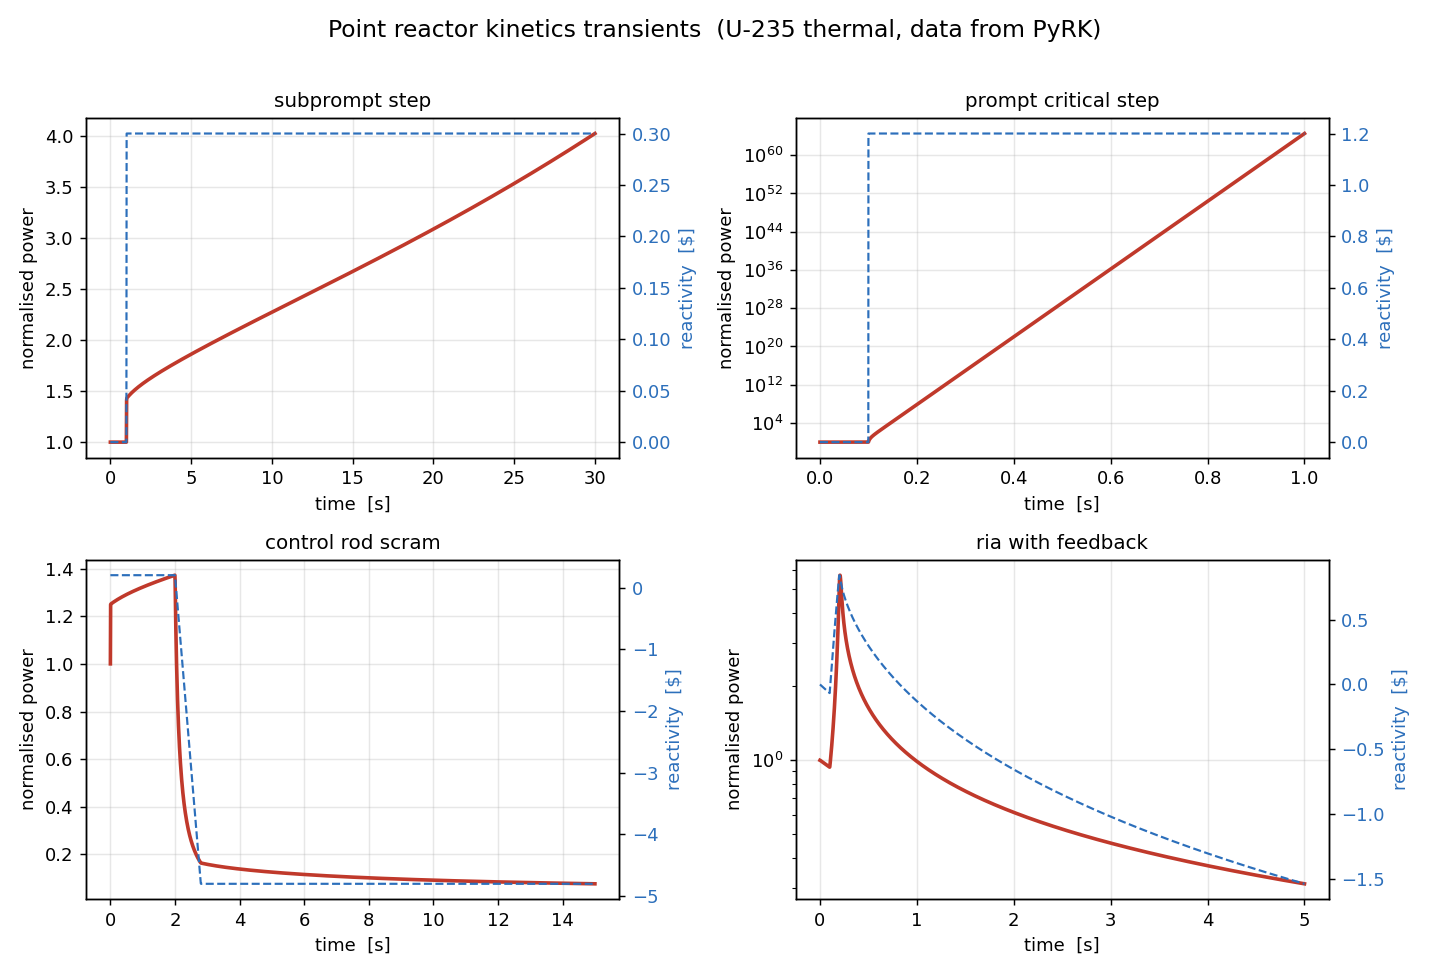
\includegraphics[width=0.62\linewidth]{figures/transients.png}\\[0.3cm]
{\footnotesize Representative point-reactor-kinetics transients computed with the
companion \texttt{reactor-kinetics} toolkit.}

\vfill
{\small This document is an educational and historical treatment of reactor
dynamics and safety. It is not a design or operating manual.\par}
\vspace{0.4cm}
{\small\today\par}
\end{titlepage}

% ===========================================================================
%  DEDICATION / EPIGRAPH
% ===========================================================================
\thispagestyle{empty}
\vspace*{4cm}
\begin{center}
{\large\itshape In memory of those who died at Chernobyl, and of the engineers\\
whose hard lessons made every reactor since a little safer.}
\end{center}
\vspace{2cm}
\begin{center}
\begin{minipage}{0.8\linewidth}\itshape\small
``Apparently, there was a widespread view that the conditions under which the
positive scram effect would be important would never occur. However, they did
appear in almost every detail in the course of the actions leading to the
Chernobyl accident.''
\begin{flushright}\normalfont\footnotesize --- IAEA, INSAG-7 (1992)\end{flushright}
\end{minipage}
\end{center}
\clearpage

% ===========================================================================
%  FRONT MATTER
% ===========================================================================
\pagenumbering{roman}

\chapter*{Abstract}
\addcontentsline{toc}{chapter}{Abstract}
Thermal stability is the property that allows a nuclear reactor to respond to
perturbations in power, temperature, and reactivity without diverging into an
uncontrolled excursion. It is the single most important dynamic characteristic
distinguishing a reactor that is safe by its very physics from one that depends
on engineered intervention to survive a transient. This monograph develops the
theory of reactor thermal stability from first principles and then uses it to
dissect the most consequential reactor accident in history---the destruction of
Chernobyl Unit~4 on 26~April 1986.

The treatment begins with the neutron balance and the point reactor kinetics
equations, including the central role of delayed neutrons, the inhour equation,
and the prompt-jump approximation. It then introduces the thermal source term,
decay heat, and the conduction--convection chain that carries fission energy
from fuel to coolant. With this groundwork, the book defines the reactivity
feedback coefficients---Doppler (fuel temperature), moderator and coolant
temperature, and the void coefficient---and shows how their signs and magnitudes
determine whether the coupled neutronic--thermal-hydraulic system is
self-correcting or self-amplifying.

A dedicated treatment of stability theory follows: linearisation of the coupled
equations, transfer functions and the Nyquist criterion, the nonlinear
Nordheim--Fuchs model of a self-limiting power excursion, and xenon-induced
spatial oscillations. The historical part surveys earlier stability-related
events (SL-1, Fermi-1, BWR oscillation events) before turning to the RBMK-1000
reactor, whose positive void coefficient and flawed control-rod design set the
stage for Chernobyl. The accident is reconstructed step by step and then
analysed through the lens of the feedback theory developed earlier, including
the evolution of the official understanding from INSAG-1 (1986) to INSAG-7
(1992). The work closes with the principles of inherent and passive safety in
modern reactor design and a computational demonstration using a companion
open-source point-kinetics toolkit.

Throughout, the emphasis is on the physical meaning of the mathematics:
\emph{a reactor is thermally stable when rising temperature removes reactivity
faster than rising power can add it.} Chernobyl is, in this language, the story
of a machine in which that inequality was reversed.


\chapter*{Preface and How to Read This Book}
\addcontentsline{toc}{chapter}{Preface}
This book is written for advanced undergraduates, graduate students, and
practising engineers who want a unified, self-contained account of why reactors
are (or are not) stable, and what happens physically when stability is lost. It
assumes a working knowledge of multivariable calculus, ordinary differential
equations, and undergraduate physics. No prior course in nuclear engineering is
strictly required: the necessary reactor physics is built up from the neutron
balance in Chapters~2 and~3.

\section*{Organisation}

The book is organised into five parts and a set of appendices.

\textbf{Part I (Foundations of Reactor Dynamics)} establishes the language:
fission, the multiplication factor and reactivity, the point reactor kinetics
equations and the indispensable role of delayed neutrons, and the decay-heat
source that persists long after the chain reaction stops.

\textbf{Part II (Heat Transport and Reactivity Feedback)} follows the energy from
its birth in the fuel to its removal by the coolant, and then introduces the
feedback coefficients that close the loop between temperature and reactivity.

\textbf{Part III (Stability Theory)} treats stability quantitatively, first by
linearisation and frequency-domain methods, then through the nonlinear physics
of power excursions, and finally through the slow, spatial instabilities driven
by xenon-135.

\textbf{Part IV (Historical Lessons)} applies the theory to real machines. After
a survey of earlier events, it examines the RBMK-1000 design in detail, then
reconstructs and analyses the Chernobyl accident.

\textbf{Part V (Modern Practice and Synthesis)} describes how the lessons are
embodied in contemporary designs that aim for inherent and passive safety, and
demonstrates the dynamics computationally before drawing the threads together.

\section*{A note on conventions}

Reactivity is expressed both as an absolute fraction $\rho$ (units of $\Delta
k/k$, often quoted in per-cent-mille, pcm, where $1\unit{pcm}=10^{-5}$) and in
\emph{dollars}, $\rho/\beta$, where $\beta$ is the total delayed-neutron
fraction. One dollar of reactivity is the boundary of prompt criticality and is
the natural yardstick for transient severity. Temperatures are in kelvin or
degrees Celsius as convenient. SI units are used throughout. Numerical examples
use validated delayed-neutron data for $^{235}$U; the full data set appears in
Appendix~A.

\section*{Companion software}

Several figures and worked transients in this book were produced with a small,
open-source point-reactor-kinetics toolkit written by the author. The code,
which couples validated kinetics data to a stiff ODE solver with temperature
feedback, is referenced in Chapter~16 and is freely available. Readers are
encouraged to reproduce and extend the examples.

\section*{Scope and disclaimer}

This is an educational and historical work. It deliberately discusses reactor
behaviour at the level of physical principle and published, openly available
engineering knowledge. It is \emph{not} an operating procedure, a design
specification, or a safety-analysis report, and nothing in it should be used as
such.


\tableofcontents
\listoffigures
\listoftables

\chapter*{Nomenclature}
\addcontentsline{toc}{chapter}{Nomenclature}
The following symbols are used throughout. Where a symbol has a conventional
secondary meaning, the intended sense is clear from context.

\begin{longtable}{p{0.16\linewidth} p{0.78\linewidth}}
\toprule
\textbf{Symbol} & \textbf{Meaning} \\
\midrule
\endhead
$\keff$ & Effective neutron multiplication factor \\
$\rho$ & Reactivity, $\rho = (\keff-1)/\keff$ \\
$\beta,\ \beta_i$ & Total and group-$i$ delayed-neutron fraction \\
$\Lambda$ & Prompt neutron generation time \\
$\ell$ & Prompt neutron lifetime \\
$\lambda_i$ & Decay constant of delayed-neutron precursor group $i$ \\
$\zeta_i,\ C_i$ & Delayed-neutron precursor concentration (group $i$) \\
$p,\ P$ & Normalised power; thermal power [W] \\
$n$ & Neutron density / population \\
$s$ & Complex frequency (Laplace variable); inverse period $1/T$ \\
$T$ & Reactor period [s] \\
$\Tf,\ \Tc$ & Fuel and coolant temperature [K] \\
$\alpha_T$ & Temperature coefficient of reactivity [$\Delta k/\mathrm{K}$] \\
$\alpha_D$ & Doppler (fuel-temperature) coefficient \\
$\alpha_v$ & Void coefficient of reactivity \\
$\alpha_P$ & Power coefficient of reactivity \\
$C,\ c_p$ & Heat capacity [J/K]; specific heat [J/(kg$\cdot$K)] \\
$h$ & Heat transfer coefficient [W/(m$^2\cdot$K)] \\
$k_f$ & Fuel thermal conductivity [W/(m$\cdot$K)] \\
$\sigma,\ \Sigma$ & Microscopic / macroscopic cross-section \\
$\phi$ & Neutron flux [n/(cm$^2\cdot$s)] \\
$I,\ X$ & Iodine-135 and Xenon-135 concentrations \\
$\gamma_I,\gamma_X$ & Fission yields of $^{135}$I and $^{135}$Xe \\
$\$$ & ``Dollar'' of reactivity, $\rho/\beta$ \\
pcm & per-cent-mille, $10^{-5}\ \Delta k/k$ \\
\bottomrule
\end{longtable}

\noindent\textbf{Selected abbreviations.}
LWR (light-water reactor), PWR (pressurised-water reactor), BWR (boiling-water
reactor), RBMK (\emph{reaktor bolshoy moshchnosti kanalnyy}, high-power
channel-type reactor), MTC (moderator temperature coefficient), FTC (fuel
temperature coefficient), ORM (operating reactivity margin), LOCA
(loss-of-coolant accident), RIA (reactivity-initiated accident), ECCS (emergency
core cooling system), SCRAM (rapid shutdown), INSAG (International Nuclear Safety
Advisory Group).


% ===========================================================================
%  MAIN MATTER
% ===========================================================================
\clearpage
\pagenumbering{arabic}

\part{Foundations of Reactor Dynamics}
\chapter{Introduction: What Stability Means for a Reactor}
\label{ch:intro}

\section{The central question}

A nuclear reactor is a device that sustains a controlled fission chain reaction
and converts the released energy into heat. The adjective \emph{controlled}
carries the entire weight of reactor engineering. An uncontrolled chain reaction
is not, in itself, exotic: it is the natural tendency of an assembly of fissile
material that is more than critical. What makes a reactor useful---and
safe---is that it can be held at a steady, prescribed power, and that when it is
disturbed it returns toward a steady state rather than running away.

This property is \textbf{thermal stability}. Informally, a reactor is thermally
stable if an increase in power produces, through the heating of its materials, a
change in conditions that tends to \emph{reduce} power again. The feedback loop
closes through temperature: power heats the fuel and coolant, and the resulting
temperature changes alter the neutron economy. If that alteration opposes the
original power change, the reactor is self-regulating; if it reinforces the
change, the reactor is unstable, and a small perturbation can grow without
bound until something physical---melting, vaporisation, mechanical
disassembly---intervenes.

\keypoint{A reactor is thermally stable when a rise in temperature removes
reactivity faster than the rise in power can add it. Stability is therefore a
statement about the \emph{sign} and \emph{magnitude} of the reactivity feedback
coefficients, weighed against the speed of the underlying neutron kinetics.}

The purpose of this book is to make that informal statement precise, to develop
the mathematics that quantifies it, and to show---through the Chernobyl
accident---what happens when the inequality is violated by design and by
operation simultaneously.

\section{Why stability is non-trivial}

It is tempting to think that stability is automatic: surely any sensible machine
settles down after a nudge. Three features of reactor physics make the question
genuinely subtle.

\textbf{First, the kinetics are fast.} The prompt neutron generation time
$\Lambda$ in a thermal reactor is of order $10^{-5}\unit{s}$ to
$10^{-4}\unit{s}$. If the chain reaction depended only on prompt neutrons, a
reactivity insertion of even a fraction of a per cent would double the power in
milliseconds---far faster than any mechanical control could respond, and far
faster than heat could redistribute to provide feedback. The reactor would be,
for practical purposes, uncontrollable.

\textbf{Second, delayed neutrons rescue controllability.} A small fraction
$\beta\approx 0.0065$ for $^{235}$U) of fission neutrons are emitted not promptly
but seconds to minutes later, from the decay of specific fission products. These
\emph{delayed neutrons} slow the effective response of the reactor by orders of
magnitude, stretching the characteristic timescale from microseconds to seconds
when the reactivity is kept below $\beta$. The entire practice of reactor
control lives in the narrow margin below one dollar of reactivity, where delayed
neutrons dominate the transient. Cross that boundary---become
\emph{prompt-critical}---and the delayed neutrons no longer matter; the reactor
reverts to its microsecond timescale. Chernobyl crossed it.

\textbf{Third, feedback is both stabilising and slow, or fast and
destabilising, depending on design.} The Doppler effect in the fuel acts almost
instantaneously because it depends on the fuel temperature, which responds
immediately to a power change. Moderator and coolant feedback are slower because
heat must first cross the fuel--clad--coolant path. Void feedback---the effect
of steam bubbles in the coolant---can be fast and, crucially, can have either
sign. Whether the \emph{net} of these effects stabilises the reactor depends on
the reactor type, the fuel loading, the coolant state, and even the point in the
fuel cycle. There is nothing automatic about it.

\section{A first picture of the feedback loop}

Figure~\ref{fig:intro-block} shows the structure we will formalise. External
reactivity (control rods, boron, operator actions) drives the neutron kinetics,
which set the power. The power deposits heat, which raises temperatures and
changes the coolant state. Those thermal changes feed back as additional
reactivity. The closed loop can be self-correcting (negative feedback) or
self-amplifying (positive feedback).

\begin{figure}[H]
\centering
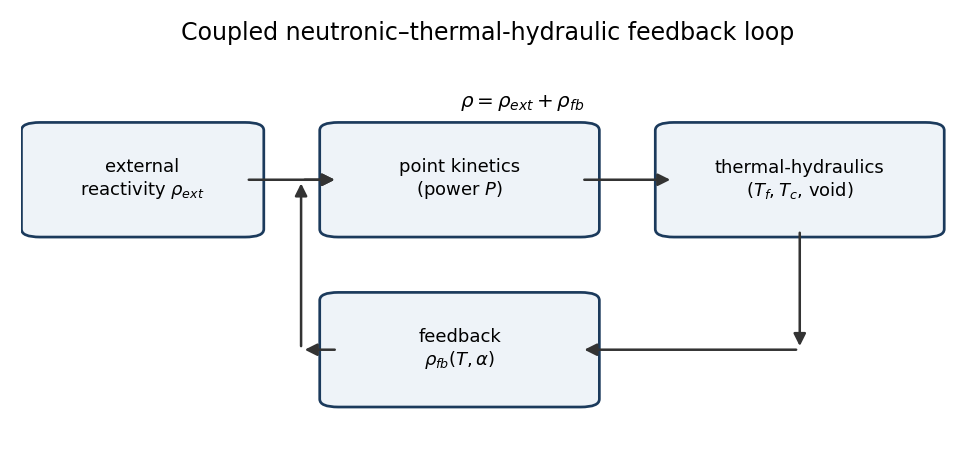
\includegraphics[width=0.95\linewidth]{figures/block.png}
\caption{The coupled neutronic--thermal-hydraulic feedback loop. The sign of the
feedback path $\rho_{fb}(T,\alpha)$ determines stability.}
\label{fig:intro-block}
\end{figure}

The mathematics of the upper path (kinetics) occupies Chapter~\ref{ch:pk}; the
right-hand block (thermal-hydraulics) occupies Chapter~\ref{ch:thermal}; the
feedback path occupies Chapter~\ref{ch:feedback}; and the behaviour of the
\emph{closed} loop---its stability---occupies Part~III.

\section{Two reactors, two fates}

To fix ideas, contrast two reactor philosophies that recur throughout the book.

A \textbf{pressurised-water reactor (PWR)} is deliberately
\emph{under-moderated}. Its lattice is designed so that if the water heats and
expands, or if it boils and forms voids, the moderation of neutrons
\emph{worsens}, the chain reaction weakens, and power falls. Both its moderator
temperature coefficient and its void coefficient are negative. Combined with a
strongly negative Doppler coefficient in the fuel, the PWR is inherently
self-regulating across its operating range: pushing the power up pushes the
temperature up, which pushes the reactivity---and hence the power---back down.

The \textbf{RBMK-1000}, the Soviet design at Chernobyl, was \emph{over-moderated}
by virtue of its large graphite moderator, which is independent of the water
coolant. In the RBMK, the water served mainly as coolant and as a neutron
\emph{absorber}. Boiling the water therefore \emph{removed an absorber} without
removing much moderation, so steam voids \emph{increased} reactivity. Its void
coefficient was strongly positive, especially at low power and with the core
configured as it was on the night of the accident. Pushing the power up boiled
more water, which pushed the reactivity---and the power---further up. The same
nudge that a PWR damps, the RBMK amplified.

\begin{figure}[H]
\centering
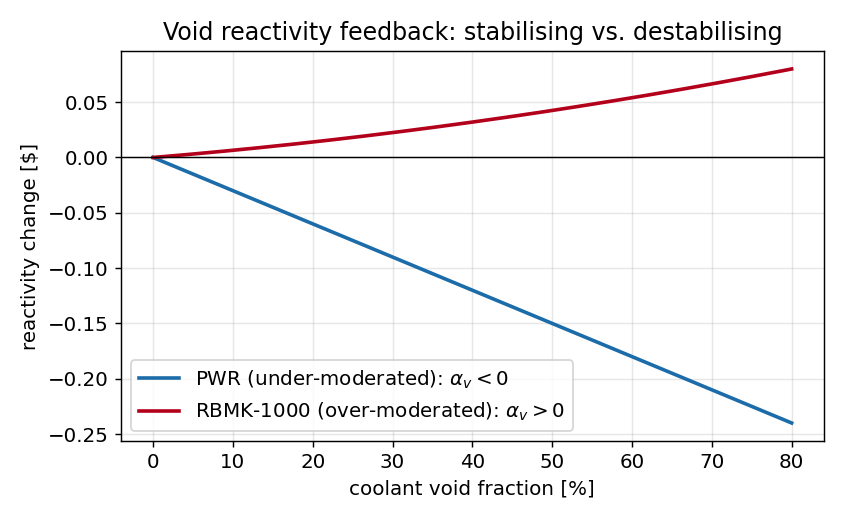
\includegraphics[width=0.78\linewidth]{figures/void.png}
\caption{Schematic void reactivity feedback. In an under-moderated lattice
(PWR) voids reduce reactivity; in an over-moderated lattice (RBMK) voids
increase it. The slope at the operating point is the void coefficient
$\alpha_v$.}
\label{fig:intro-void}
\end{figure}

This single contrast---under-moderated versus over-moderated, negative versus
positive void coefficient---is the physical heart of the Chernobyl story, and we
will return to it repeatedly with increasing precision.

\section{What ``thermal'' stability is not}

It is worth separating thermal stability from several neighbouring concepts that
are sometimes conflated with it.

\emph{Criticality} is a static balance: $\keff=1$, neutron production equals
neutron loss. A reactor can be exactly critical and still be dynamically
unstable. Stability is about what happens to small departures from balance, not
about the balance itself.

\emph{Controllability} is the ability of operators and automatic systems to
drive the reactor to a desired state. A reactor can be controllable yet rely on
that control to remain safe; the ideal is a reactor whose physics keep it safe
even when control fails. Inherent stability reduces the burden on control.

\emph{Thermal-hydraulic stability} in the narrow sense refers to flow and
boiling instabilities (density-wave oscillations, flow excursions) that can
occur even at fixed power. These couple strongly to neutronics in boiling
systems and are part of the broader stability picture treated in
Chapter~\ref{ch:linear}.

\emph{Structural and material stability}---the integrity of fuel, cladding, and
pressure boundary under thermal stress---is the ultimate limit that a power
excursion challenges. Thermal stability theory predicts whether and how fast a
reactor approaches those limits.

\section{Roadmap and how the Chernobyl thread runs through the book}

Each part of this book develops a piece of theory and then points it at
Chernobyl. Part~I gives us the kinetics that explain why the final excursion was
a prompt-critical event measured in seconds. Part~II gives us the feedback
coefficients that explain why the RBMK amplified rather than damped the
disturbance. Part~III gives us the stability criteria that, applied to the
RBMK's operating state that night, predict instability. Part~IV reconstructs the
accident and shows the theory accounting for it in detail. Part~V asks how modern
designs build in the negative feedback that the RBMK lacked, and demonstrates the
dynamics with a small open-source kinetics code.

The recurring lesson is not that the operators were uniquely reckless or that one
component uniquely failed. It is that a reactor with the wrong sign of feedback,
operated into the corner of its envelope where that wrong sign was strongest,
behaved exactly as the equations say such a machine must. Stability is physics;
the accident was the physics asserting itself.


\section*{Exercises}
\addcontentsline{toc}{section}{Exercises}
\begin{enumerate}[leftmargin=*,itemsep=2pt]
\item Explain in one sentence the difference between criticality and stability, and give an example of a reactor state that is critical but unstable.
\item A reactor has a positive void coefficient. Describe qualitatively the sequence of events following a small increase in power, and contrast it with a reactor having a negative void coefficient.
\item Why is it insufficient for a reactor merely to ``settle down'' after a disturbance for it to be called inherently safe? Distinguish stability from controllability.
\item List the three features of reactor physics that make stability non-trivial, and explain which one delayed neutrons mitigate.
\item Using the under-/over-moderated distinction, explain why a PWR and an RBMK respond oppositely to coolant boiling.
\end{enumerate}

\chapter{Reactor Physics Fundamentals}
\label{ch:physics}

This chapter assembles the minimum reactor physics needed for a dynamic theory:
fission and the neutron balance, the multiplication factor and reactivity, the
six-factor formula, and the meaning of the neutron lifetime. Readers with a
background in nuclear engineering may skim it; the notation introduced here is
used everywhere later.

\section{Fission and the neutron economy}

When a $^{235}$U nucleus absorbs a thermal neutron it may fission, splitting into
two fragments and releasing on average $\nu\approx 2.43$ prompt neutrons together
with about $200\unit{MeV}$ of energy. The energy is distributed roughly as
$168\unit{MeV}$ in the kinetic energy of the fragments (deposited essentially at
the point of fission, in the fuel), with the remainder in prompt neutrons,
prompt gamma rays, and---importantly for later---the radioactive decay of the
fission products. Of the recoverable energy, about $93\%$ appears promptly and
about $7\%$ is released later as decay heat (Chapter~\ref{ch:decay}).

A self-sustaining chain reaction requires that, on average, exactly one of the
$\nu$ neutrons from each fission goes on to cause another fission. The other
neutrons are lost to non-fission capture (in fuel, moderator, coolant,
structure, and control materials) or to leakage out of the core. The bookkeeping
of these gains and losses is the neutron economy.

\section{The multiplication factor and reactivity}

Define the effective multiplication factor
\begin{equation}
\keff = \frac{\text{neutrons produced in one generation}}
             {\text{neutrons lost (absorbed + leaked) in the preceding generation}}.
\end{equation}
The three regimes are
\begin{equation}
\keff < 1 \ (\text{subcritical}),\qquad
\keff = 1 \ (\text{critical}),\qquad
\keff > 1 \ (\text{supercritical}).
\end{equation}
A critical reactor sustains a constant population; a supercritical one grows.

Because the interesting dynamics involve small departures from criticality, it is
convenient to measure the distance from $\keff=1$ directly. The
\textbf{reactivity} is
\begin{equation}
\boxed{\ \rho \equiv \frac{\keff-1}{\keff}\ }
\label{eq:reactivity}
\end{equation}
which is dimensionless, zero at criticality, positive above it, and negative
below. Reactivity is small in practice: a useful operating insertion might be a
few hundred pcm (recall $1\unit{pcm}=10^{-5}$), and one ``dollar'' equals
$\beta\approx 650\unit{pcm}$ for $^{235}$U. We will almost always work to first
order in $\rho$, where $\rho\approx \keff-1$.

\begin{definition}[Reactivity in dollars]
The reactivity expressed in units of the delayed-neutron fraction,
$\$\equiv \rho/\beta$, is the natural measure of transient severity. At
$\rho=\beta$ ($\$=1$) the reactor is prompt-critical: the prompt neutrons alone
sustain the chain, and delayed neutrons are no longer needed to maintain
growth.
\end{definition}

\section{The six-factor formula}

The effective multiplication factor for a finite thermal reactor factors into six
physically distinct processes:
\begin{equation}
\keff = \eta\, f\, p\, \varepsilon\, P_{\!f}\, P_{\!t},
\label{eq:sixfactor}
\end{equation}
where
\begin{itemize}[nosep]
\item $\eta$ is the reproduction factor (neutrons produced per thermal neutron
absorbed in fuel);
\item $f$ is the thermal utilisation (fraction of thermal absorptions occurring
in fuel rather than in moderator, coolant, or structure);
\item $p$ is the resonance escape probability (fraction of neutrons that slow
past the $^{238}$U capture resonances without being absorbed);
\item $\varepsilon$ is the fast-fission factor (a small boost from fissions
caused by fast neutrons);
\item $P_{\!f}$ and $P_{\!t}$ are the fast and thermal non-leakage
probabilities.
\end{itemize}
The product $\eta f p \varepsilon$ is the infinite-medium multiplication factor
$k_\infty$, and $\keff = k_\infty P_{\!f} P_{\!t}$.

The value of the six-factor formula for our purposes is that it localises
feedback. Temperature and voids do not change $\keff$ abstractly; they change
\emph{specific factors}. The Doppler effect (Chapter~\ref{ch:feedback}) acts on
the resonance escape probability $p$ through the broadening of the $^{238}$U
resonances. Moderator heating and voiding act on $f$ and $p$ through changes in
moderator density and the moderation ratio. Expansion changes leakage,
$P_{\!f}P_{\!t}$. Tracking \emph{which} factor a given feedback alters, and with
\emph{which sign}, is the discipline that distinguishes a stable lattice from an
unstable one.

\keypoint{Whether a reactor is under- or over-moderated is, in six-factor terms,
a competition: voiding the coolant tends to raise $p$ (less parasitic capture
and resonance absorption) but lower $f$ and worsen moderation. In an
under-moderated lattice the harmful effects win and reactivity falls; in an
over-moderated lattice (like the RBMK with its graphite) the helpful effect on
$p$ and the loss of the water absorber win, and reactivity rises.}

\section{The neutron lifetime and generation time}

Two closely related timescales govern how fast the population responds.

The \textbf{prompt neutron lifetime} $\ell$ is the mean time from a neutron's
birth to its absorption or leakage. In a thermal reactor it is dominated by the
slowing-down time plus the thermal diffusion time and is of order
$10^{-4}\unit{s}$ in a light-water reactor, somewhat longer in a graphite system.

The \textbf{prompt neutron generation time} is
\begin{equation}
\Lambda = \frac{\ell}{\keff}\approx \ell \quad(\keff\approx 1),
\end{equation}
the mean time between successive neutron generations. We use $\Lambda$ in the
kinetics equations; for $^{235}$U thermal systems a representative value is
$\Lambda\sim 10^{-5}\!-\!10^{-4}\unit{s}$. Its smallness is precisely why prompt
supercriticality is so dangerous: with $\Lambda=10^{-5}\unit{s}$ and a prompt
reactivity of just $0.2\%$, the prompt growth rate is
$\rho_{\text{prompt}}/\Lambda\sim 200\unit{s^{-1}}$, an e-folding every
$5\unit{ms}$.

\section{Neutron flux, cross-sections, and reaction rates}

The neutron flux $\phi(\mathbf r,E,t)$ is the product of neutron density and
speed; it measures the rate at which neutrons traverse unit area. Reaction rates
are products of flux and macroscopic cross-section,
\begin{equation}
R_x = \Sigma_x \phi, \qquad \Sigma_x = N\sigma_x,
\end{equation}
where $N$ is the number density of nuclei and $\sigma_x$ the microscopic
cross-section for reaction $x$ (fission, capture, scattering). Cross-sections
depend strongly on neutron energy; the resonance structure of $^{238}$U capture
near a few eV, and the $1/v$ behaviour of many thermal absorbers, are central to
feedback and to xenon poisoning respectively.

The fission power density is
\begin{equation}
q'''(\mathbf r,t) = E_f\, \Sigma_f\, \phi(\mathbf r,t),
\end{equation}
with $E_f\approx 200\unit{MeV}$ the recoverable energy per fission. Integrated
over the core, this is the thermal power that the kinetics equations track and
that the thermal-hydraulic system must remove.

\section{From the transport equation to point kinetics}

The full description of the neutron field is the time-dependent neutron transport
(or, in diffusion approximation, the neutron diffusion) equation, a
seven-dimensional integro-differential equation in space, energy, angle, and
time. For stability analysis we usually do not need its full spatial detail.
If the spatial shape of the flux changes slowly compared with its amplitude---the
\emph{point} approximation---we can separate variables,
\begin{equation}
\phi(\mathbf r,E,t)\approx \psi(\mathbf r,E)\, n(t),
\end{equation}
and reduce the dynamics to ordinary differential equations for the amplitude
$n(t)$ and the delayed-neutron precursors. This reduction yields the point
reactor kinetics equations of Chapter~\ref{ch:pk}. The approximation is excellent
for compact cores responding coherently, and it is the workhorse of reactor
dynamics. Its principal failure---when different regions of a large core behave
differently---gives rise to the spatial instabilities of
Chapter~\ref{ch:xenon}, and was a real complicating factor in the large RBMK core
at Chernobyl, where the point picture understates the danger of an asymmetric,
axially-peaked flux.


\section*{Exercises}
\addcontentsline{toc}{section}{Exercises}
\begin{enumerate}[leftmargin=*,itemsep=2pt]
\item Starting from $\keff=1.002$, compute the reactivity $\rho$ in pcm and in dollars (take $\beta=0.0065$).
\item Using the six-factor formula, identify which factor the Doppler effect modifies and with what sign.
\item Estimate the prompt growth rate $\rho_{\text{prompt}}/\Lambda$ for $\rho_{\text{prompt}}=0.003$ and $\Lambda=10^{-5}\,$s, and the corresponding e-folding time.
\item Explain physically why voiding an over-moderated lattice raises the resonance escape probability $p$.
\item Why does the point-kinetics approximation fail for large cores, and what phenomenon (Chapter 10) results?
\end{enumerate}

\chapter{Point Reactor Kinetics}
\label{ch:pk}

The point reactor kinetics (PRK) equations are the dynamical backbone of this
book. They describe how reactor power evolves in time under a prescribed
reactivity, and they make explicit the decisive role of delayed neutrons. We
derive them, solve them in the cases that matter for stability, and extract the
two results---the inhour equation and the prompt-jump approximation---that we
will use again and again.

\section{Delayed neutrons}

Most fission neutrons are emitted within $10^{-14}\unit{s}$ of fission: these are
\emph{prompt}. A small fraction, however, appear with a delay, emitted by certain
neutron-rich fission products (``precursors'') as they beta-decay. The classic
example is $^{87}$Br, which decays to an excited $^{87}$Kr that promptly emits a
neutron; the effective delay is set by the $55\unit{s}$ half-life of the bromine.
In practice the many precursors are grouped into six (sometimes eight) effective
groups, each with a yield fraction $\beta_i$ and a decay constant $\lambda_i$.

The total delayed fraction is
\begin{equation}
\beta = \sum_{i=1}^{6}\beta_i \approx 0.0065 \ \text{for }^{235}\text{U (thermal)},
\end{equation}
with group decay constants ranging from $\lambda_1\approx0.0124\unit{s^{-1}}$
(half-life $\sim 56\unit{s}$) to $\lambda_6\approx 3.0\!-\!3.9\unit{s^{-1}}$
(half-life under a second). Although less than one neutron in a hundred is
delayed, these neutrons set the timescale of the controllable reactor: their
mean delay, of order $10\unit{s}$, vastly exceeds the prompt generation time
$\Lambda\sim 10^{-5}\unit{s}$, so the \emph{average} neutron lifetime weighted by
prompt and delayed contributions is dominated by the delayed term whenever the
reactor is below prompt criticality. Appendix~A lists the full data set.

\section{Derivation of the PRK equations}

Let $n(t)$ be the neutron population (proportional to power $P$) and $C_i(t)$ the
concentration of precursor group $i$. In one generation, $\keff$ neutrons are
produced per neutron; of these, a fraction $(1-\beta)$ are prompt and a fraction
$\beta_i$ feed precursor group $i$. The prompt balance gives a production rate
$(1-\beta)\keff n/\ell$ against a loss rate $n/\ell$, while each precursor group
gains at rate $\beta_i \keff n/\ell$ and loses by decay at rate $\lambda_i C_i$;
the decay of precursors returns neutrons at rate $\lambda_i C_i$. Writing
$\Lambda=\ell/\keff$ and using $\rho=(\keff-1)/\keff$, the result is the standard
six-group point reactor kinetics equations:
\begin{equation}
\boxed{\;
\begin{aligned}
\frac{\dd n}{\dd t}
  &= \frac{\rho(t)-\beta}{\Lambda}\, n(t) + \sum_{i=1}^{6}\lambda_i C_i(t),\\[4pt]
\frac{\dd C_i}{\dd t}
  &= \frac{\beta_i}{\Lambda}\, n(t) - \lambda_i C_i(t),
  \qquad i=1,\dots,6.
\end{aligned}\;}
\label{eq:prk}
\end{equation}
The same equations hold with $n$ replaced by power $P$, since the two are
proportional in the point approximation. In normalised form we write $p=P/P_0$.

The structure of \eqref{eq:prk} is already revealing. The prompt coefficient
$(\rho-\beta)/\Lambda$ changes sign at $\rho=\beta$. Below it, the coefficient is
\emph{negative}: the prompt chain alone would die away, and the population is held
up only by the slow return of delayed neutrons through $\sum\lambda_iC_i$. This
is the regime of controllable operation. Above it, $\rho>\beta$, the prompt
coefficient is positive and the population grows on the $\Lambda$ timescale
regardless of the delayed neutrons---prompt criticality.

\section{Steady state and the initial condition}

At constant power $p_0$ with $\rho=0$, the time derivatives vanish and
\begin{equation}
C_{i,0} = \frac{\beta_i}{\lambda_i\Lambda}\, p_0,
\label{eq:prk-ss}
\end{equation}
which is the equilibrium precursor inventory. The precursors hold a large reservoir
of ``stored'' delayed neutrons: because $\lambda_i\Lambda\ll\beta_i$, the
equilibrium $C_{i,0}$ greatly exceeds $p_0$. This reservoir is what gives the
reactor its inertia and is the physical reason the prompt-jump (below) is finite.

\section{The prompt jump approximation}

Consider a step insertion of reactivity $\rho<\beta$ at $t=0$ on a reactor at
steady power. Immediately after the step, the precursor concentrations cannot
change instantaneously (they evolve on the slow $\lambda_i$ timescale), so the
$\sum\lambda_iC_i$ term is momentarily fixed at its pre-step value. The fast
prompt dynamics then drive $n$ to a new quasi-equilibrium on the $\Lambda$
timescale. Setting $\dd n/\dd t\to 0$ in \eqref{eq:prk} with the precursor term
held fixed yields the \textbf{prompt-jump approximation}:
\begin{equation}
\boxed{\ \frac{n(0^+)}{n(0^-)} = \frac{\beta}{\beta-\rho}\ }
\label{eq:promptjump}
\end{equation}
The power jumps essentially instantly by this factor, then rises (or falls) more
slowly as the precursors readjust. For $\rho=0.5\$$ ($\rho=0.5\beta$) the jump is
a factor of two; as $\rho\to\beta^-$ the predicted jump diverges, signalling the
breakdown of the approximation and the onset of prompt criticality. The
prompt-jump captures the ``instant'' part of a transient and is invaluable for
estimating the immediate consequence of a reactivity insertion.

\section{The inhour equation}

To find the asymptotic behaviour, seek exponential solutions $n,C_i\propto
e^{st}$ for constant $\rho$. Substituting into \eqref{eq:prk} gives
$C_i = \beta_i n/[\Lambda(s+\lambda_i)]$, and \eqref{eq:prk} becomes the
\textbf{inhour equation}:
\begin{equation}
\boxed{\ \rho = \Lambda s + \sum_{i=1}^{6}\frac{\beta_i\, s}{s+\lambda_i}\ }
\label{eq:inhour}
\end{equation}
This transcendental equation has seven real roots $s_j$ for six delayed groups.
The roots interlace the negative poles $-\lambda_i$; six of them are negative
(decaying transients), and one---the \emph{dominant} root---has the sign of
$\rho$. The reactor period is $T=1/s_{\text{dominant}}$, the time for the power to
change by a factor $e$.

For small positive reactivity the dominant root is small, $s\approx
\rho/(\beta-\rho)\cdot \bar\lambda^{-1}$ in a one-group caricature, giving a long
(stable, slow) period dominated by the delayed neutrons. As $\rho\to\beta$ the
dominant root grows rapidly and the period collapses; beyond $\beta$ the leading
behaviour is $s\approx(\rho-\beta)/\Lambda$, the prompt period.

\begin{figure}[H]
\centering
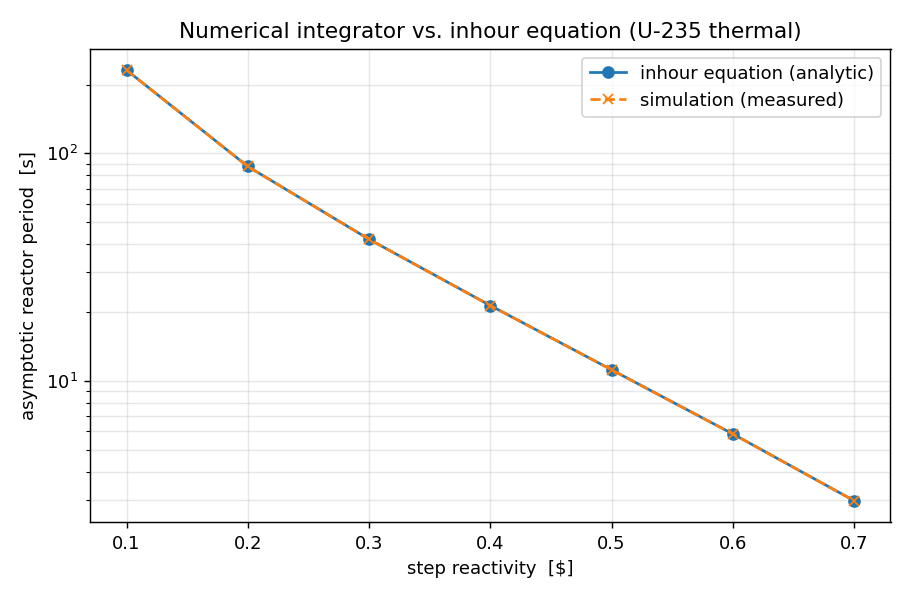
\includegraphics[width=0.74\linewidth]{figures/inhour_validation.png}
\caption{Asymptotic reactor period as a function of step reactivity for
$^{235}$U thermal data. The closed-form inhour solution (solid) and a direct
numerical integration of \eqref{eq:prk} (dashed) agree to
better than $10^{-4}$. Note the steep collapse of the period as reactivity
approaches one dollar.}
\label{fig:inhour}
\end{figure}

\begin{example}[The danger of one dollar]
With $\Lambda=10^{-5}\unit{s}$ and $\beta=0.0065$, a reactivity of
$0.5\$=325\unit{pcm}$ gives a stable period of tens of seconds---easily
controllable. A reactivity of $1.5\$=975\unit{pcm}$ is $0.5\$$ above prompt
critical; the dominant root is approximately
$s\approx(\rho-\beta)/\Lambda=(0.00975-0.0065)/10^{-5}\approx 325\unit{s^{-1}}$,
an e-folding every $3\unit{ms}$. Power rises by a factor of $e^{10}\approx
2\times10^{4}$ in just $30\unit{ms}$. No mechanical system can intervene on that
timescale; only the prompt negative feedback of the fuel (Doppler) can, if it
exists and has the right sign.
\end{example}

\section{Numerical solution and stiffness}

For time-varying $\rho(t)$, or with feedback, \eqref{eq:prk}
must be integrated numerically. The system is \emph{stiff}: it contains the very
fast prompt timescale $\Lambda$ alongside the slow precursor timescales
$1/\lambda_i$, spanning six orders of magnitude. Explicit integrators require
prohibitively small steps; implicit or specialised stiff methods (backward
differentiation, LSODA, or analytic-within-a-step schemes) are standard.
Figure~\ref{fig:transients} shows representative transients computed this way:
a sub-prompt step settling onto a stable period, a prompt-critical excursion
diverging on the millisecond scale, a control-rod scram, and---most
importantly for stability---a reactivity-initiated transient that is turned over
by negative temperature feedback. The last of these is the prototype of a
\emph{thermally stable} response, and the contrast with the un-fed-back
prompt-critical case is the whole subject of the book in one picture.

\begin{figure}[H]
\centering
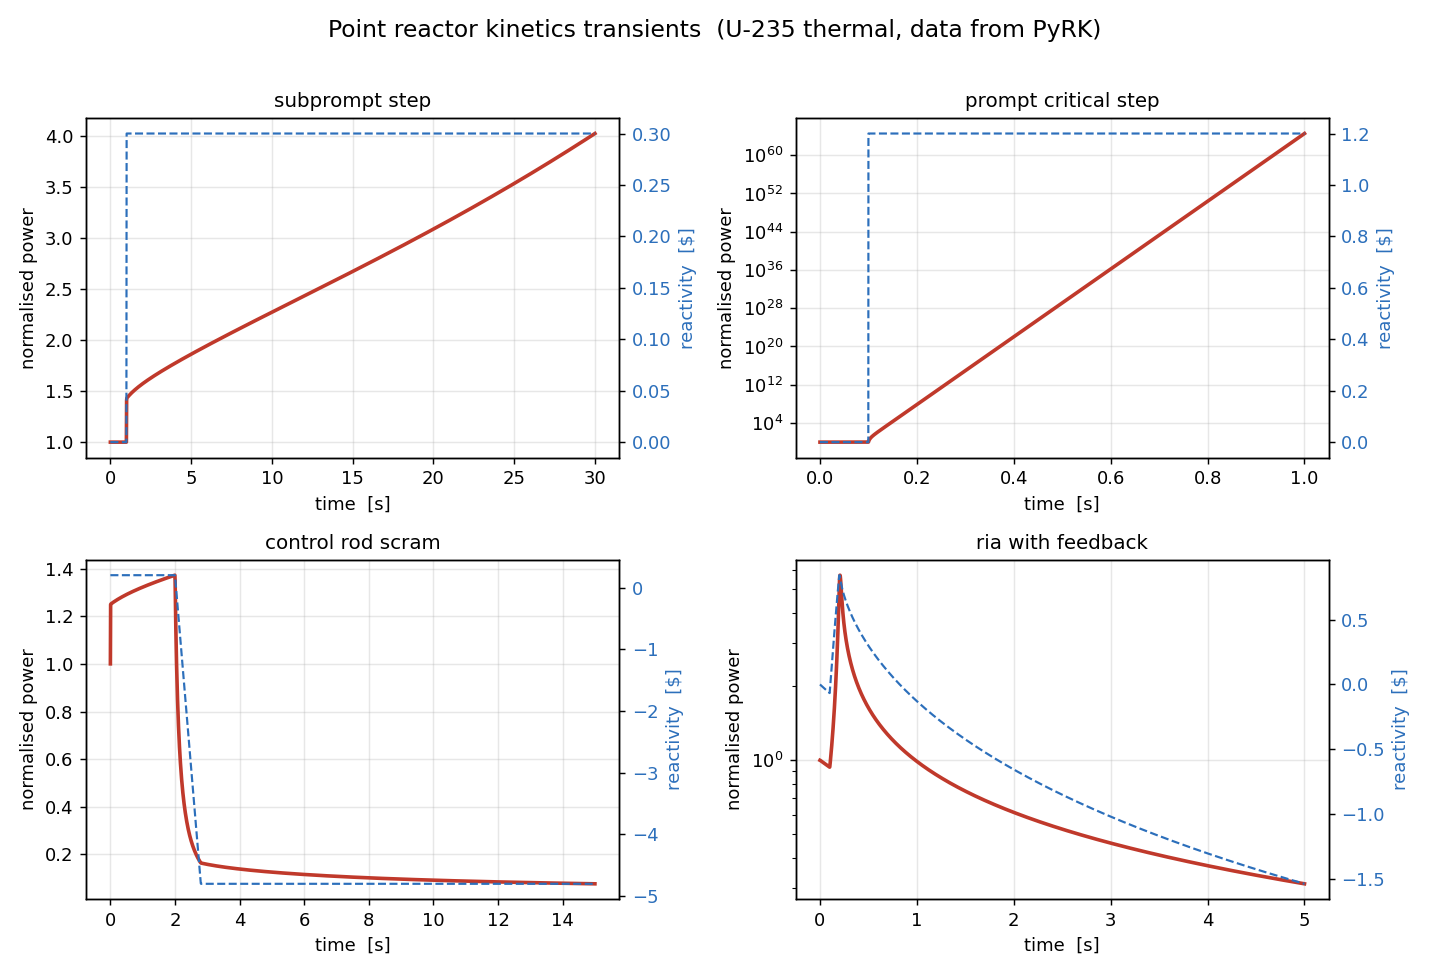
\includegraphics[width=\linewidth]{figures/transients.png}
\caption{Point-kinetics transients for $^{235}$U thermal data. Top left: a
sub-prompt $+0.3\$$ step (stable period). Top right: a prompt-critical $+1.2\$$
step (runaway, log scale). Bottom left: a control-rod scram. Bottom right: a
reactivity-initiated excursion limited by negative feedback---the signature of
thermal stability.}
\label{fig:transients}
\end{figure}

\keypoint{The point kinetics equations contain the entire timescale problem of
reactor control. Below one dollar, delayed neutrons stretch the response to
seconds and the reactor is controllable. Above one dollar, the response collapses
to the prompt timescale and only instantaneous feedback can save the reactor.
Everything that follows---feedback coefficients, stability criteria, the
Chernobyl excursion---is about staying below that line, or about what happens
when a machine crosses it.}



\section{Matrix formulation and spectral theory}
\label{sec:pk-matrix}

Write the state $\mathbf y=(n,C_1,\dots,C_G)^{\!\top}\in\mathbb R^{G+1}$. For
constant $\rho$ the point kinetics \eqref{eq:prk} are the linear system
$\dot{\mathbf y}=\mathbf M(\rho)\mathbf y$ with
\begin{equation}
\mathbf M(\rho)=
\begin{pmatrix}
\dfrac{\rho-\beta}{\Lambda} & \lambda_1 & \cdots & \lambda_G\\[5pt]
\dfrac{\beta_1}{\Lambda} & -\lambda_1 & & \\
\vdots & & \ddots & \\
\dfrac{\beta_G}{\Lambda} & & & -\lambda_G
\end{pmatrix}.
\label{eq:M}
\end{equation}

\begin{theorem}[Spectrum equals inhour roots]
\label{thm:spectrum}
$s\in\sigma(\mathbf M(\rho))$ if and only if $s$ solves the inhour equation
\eqref{eq:inhour}: $\ \rho=\Lambda s+\sum_{i=1}^G \beta_i s/(s+\lambda_i).$
\end{theorem}
\begin{proof}
For an eigenpair $(s,\mathbf y)$ the precursor rows give
$C_i=\frac{\beta_i}{\Lambda(s+\lambda_i)}\,n$ (for $s\ne-\lambda_i$), and the first
row gives $s\,n=\frac{\rho-\beta}{\Lambda}n+\sum_i\lambda_i C_i$. Substituting and
dividing by $n/\Lambda$,
$\Lambda s=\rho-\beta+\sum_i\frac{\lambda_i\beta_i}{s+\lambda_i}$; using
$\lambda_i/(s+\lambda_i)=1-s/(s+\lambda_i)$ yields \eqref{eq:inhour}. The poles
$s=-\lambda_i$ are not eigenvalues (they force $n=0$ and hence $\mathbf y=0$).
\end{proof}

\begin{theorem}[Reality, simplicity, interlacing]
\label{thm:interlacing}
For $\rho\ne0$ the inhour equation has exactly $G+1$ real simple roots
$s_0>s_1>\cdots>s_G$ obeying
$s_0>-\lambda_{(1)}>s_1>-\lambda_{(2)}>\cdots>-\lambda_{(G)}>s_G$, where
$\lambda_{(1)}<\cdots<\lambda_{(G)}$ are the ordered decay constants. Moreover
$\operatorname{sign}(s_0)=\operatorname{sign}(\rho)$.
\end{theorem}
\begin{proof}
Let $h(s)=\Lambda s+\sum_i\beta_i s/(s+\lambda_i)$. Then
$h'(s)=\Lambda+\sum_i\beta_i\lambda_i/(s+\lambda_i)^2>0$ wherever defined, so $h$
is strictly increasing on each interval between consecutive poles, running from
$-\infty$ to $+\infty$ across each; thus $h(s)=\rho$ has exactly one root in each of
the $G$ inter-pole gaps and one to the right of $-\lambda_{(1)}$, giving $G+1$
simple real interlacing roots. Since $h(0)=0$ and $h$ is increasing through the
origin, $\rho>0\Rightarrow s_0>0$ and $\rho<0\Rightarrow s_0<0$.
\end{proof}

\begin{corollary}
The asymptotic period $T=1/s_0$ has the sign of $\rho$, and the solution is
$\mathbf y(t)=\sum_{j=0}^{G}c_j\mathbf v_j e^{s_j t}$ with $\mathbf v_j$ the
eigenvector of $s_j$; for $t\to\infty$ the dominant mode $e^{s_0 t}$ prevails.
\end{corollary}

\begin{proposition}[Nonnegativity of the flow]
\label{prop:metzler}
$\mathbf M(\rho)$ is a Metzler matrix (off-diagonal entries $\ge0$); hence
$e^{\mathbf M t}\ge0$ entrywise for $t\ge0$, and $\mathbf y(0)\ge0$ implies
$\mathbf y(t)\ge0$ for all $t\ge0$. In particular the power $n(t)$ never goes
negative.
\end{proposition}
\begin{proof}
The off-diagonal entries are $\lambda_i\ge0$ and $\beta_i/\Lambda\ge0$; all other
off-diagonal entries vanish. Choose $c>0$ with $\mathbf M+c\mathbf I\ge0$; then
$e^{\mathbf M t}=e^{-ct}e^{(\mathbf M+c\mathbf I)t}$, and the exponential of a
nonnegative matrix is nonnegative (its power series has nonnegative terms). A
nonnegative semigroup maps the nonnegative orthant into itself.
\end{proof}

\paragraph{Prompt jump as a singular perturbation.}
Treat $\Lambda$ as a small parameter. The fast equation
$\Lambda\dot n=(\rho-\beta)n+\Lambda\sum_i\lambda_i C_i$ has, for $\rho<\beta$, a
boundary layer of width $\mathcal O\!\big(\Lambda/(\beta-\rho)\big)$ during which
the slow variables $C_i$ are frozen at their pre-step values. Matching the inner
(layer) solution to the outer quasi-static balance
$n=\Lambda\big(\sum_i\lambda_iC_i\big)/(\beta-\rho)$ gives, at $t=0^+$,
$n(0^+)/n(0^-)=\beta/(\beta-\rho)$, i.e.\ \eqref{eq:promptjump}, with relative error
$\mathcal O(\Lambda)$. This places the prompt-jump approximation on a rigorous
asymptotic footing.


\section*{Exercises}
\addcontentsline{toc}{section}{Exercises}
\begin{enumerate}[leftmargin=*,itemsep=2pt]
\item Derive the steady-state precursor concentration \eqref{eq:prk-ss} from the precursor equation.
\item Compute the prompt-jump factor for $\rho=0.25\$$ and for $\rho=0.9\$$. Comment on the trend as $\rho\to\beta$.
\item Show that the inhour equation \eqref{eq:inhour} has exactly $G+1$ real roots for $G$ delayed groups.
\item For $\rho=1.5\$$, $\Lambda=10^{-5}\,$s, $\beta=0.0065$, estimate the prompt period and the factor by which power grows in $20\,$ms.
\item Explain why the point-kinetics system is numerically stiff and why explicit integrators struggle with it.
\end{enumerate}

\chapter{Decay Heat: The Source That Will Not Switch Off}
\label{ch:decay}

\section{Why decay heat matters for stability and safety}

The point kinetics equations describe the \emph{fission} power, which responds
within seconds to a scram. But roughly $7\%$ of a reactor's steady-state thermal
power comes not from fission directly but from the radioactive decay of fission
products accumulated in the fuel. This \textbf{decay heat} cannot be switched off
by inserting control rods: it is governed by the half-lives of hundreds of
nuclides and decays only with time. Immediately after shutdown from full power,
decay heat is about $6\!-\!7\%$ of the previous power; it falls to roughly $1\%$
after an hour and continues to decline over days. For a $3000\unit{MW}$ thermal
core, $7\%$ is $210\unit{MW}$---a space-heater the size of a small power
station that turns on the instant you shut the reactor down and that must be
removed continuously to prevent the fuel from melting.

Decay heat is the reason a reactor is never truly ``off'' from a thermal
standpoint, and it is the link between a reactivity transient and a thermal
catastrophe: at Chernobyl, at Three Mile Island, and at Fukushima, decay heat
was the persistent source that turned a loss of cooling into core damage. For
stability theory it matters because it sets a floor on the thermal source term
and because, in fast transients, a small additional decay-heat contribution adds
to the energy that feedback must absorb.

\section{The Way--Wigner correlation}

A classic engineering estimate of decay power after an infinitely long
irradiation is the Way--Wigner correlation,
\begin{equation}
\frac{P_d(t)}{P_0} \approx 0.066\left[\,t^{-0.2} - (t+t_0)^{-0.2}\,\right],
\label{eq:waywigner}
\end{equation}
where $t$ is the time since shutdown and $t_0$ the operating time, both in
seconds. For $t_0\to\infty$ this reduces to $P_d/P_0\approx 0.066\,t^{-0.2}$.
Figure~\ref{fig:decay} plots this approximation. The slow, power-law decline---a
consequence of the broad distribution of fission-product half-lives---is the
defining feature: there is no single time constant, and the heat lingers for a
long time.

\begin{figure}[H]
\centering
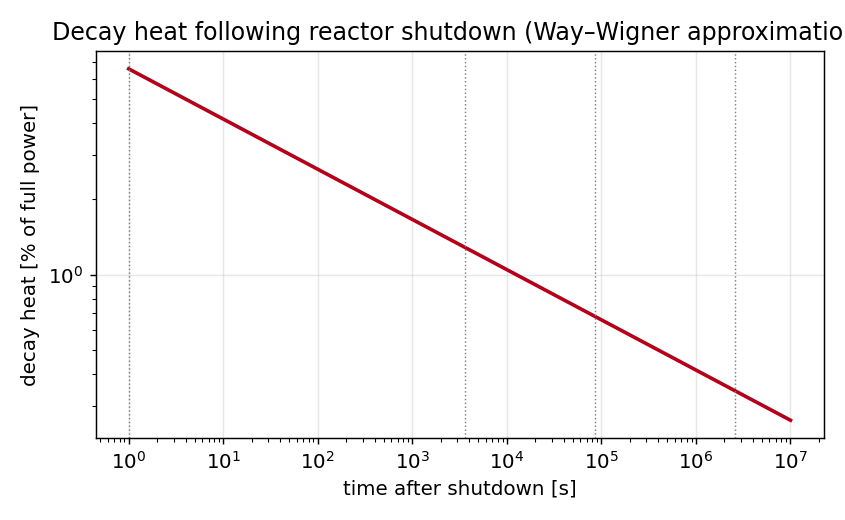
\includegraphics[width=0.74\linewidth]{figures/decay_heat.png}
\caption{Decay heat as a fraction of full power following shutdown, from the
Way--Wigner approximation \eqref{eq:waywigner}. The power-law tail reflects the
broad spectrum of fission-product half-lives; the heat cannot be turned off,
only waited out and removed.}
\label{fig:decay}
\end{figure}

More accurate standards (ANSI/ANS-5.1) sum contributions from the major
fissioning nuclides ($^{235}$U, $^{239}$Pu, $^{238}$U) with tabulated
coefficients, and add the actinide contributions from $^{239}$U and $^{239}$Np,
which are significant in the first day. For our purposes the Way--Wigner picture
captures the essential physics: a large, slowly decaying, irreducible source.

\section{Decay heat in the kinetics model}

Decay heat can be appended to the point kinetics framework with its own set of
decay-heat groups $\omega_k$, in direct analogy with the precursors:
\begin{equation}
P_{\text{total}}(t) = P_f(t) + \sum_k \omega_k(t),\qquad
\frac{\dd \omega_k}{\dd t} = \kappa_k P_f(t) - \lambda_k^{(d)}\omega_k(t),
\end{equation}
where $\kappa_k$ are the energy fractions and $\lambda_k^{(d)}$ the decay-heat
group constants. In a fast power transient the fission term $P_f$ dominates and
decay heat is a small correction; in the aftermath of a scram it is the only term
left. The companion software of Chapter~\ref{ch:comp} includes decay-heat groups
for exactly this reason.

\section{The thermal consequence: a worked estimate}

\begin{example}[Adiabatic heat-up after loss of cooling]
Suppose cooling is lost just after shutdown from full power $P_0$, and decay heat
is initially $q=0.06\,P_0$. If the core thermal mass is $C$ and no heat is
removed, the fuel temperature rises at
\begin{equation}
\frac{\dd \Tf}{\dd t} = \frac{q}{C}.
\end{equation}
For a core with $C\sim 10^{7}\unit{J/K}$ and $P_0=3\times10^{9}\unit{W}$, the
initial decay power is $q\approx 1.8\times10^{8}\unit{W}$, so
$\dd\Tf/\dd t\approx 18\unit{K/s}$. Starting near the normal operating
temperature, the fuel would reach the melting point of $\mathrm{UO_2}$
($\sim 2800\degC$) in a few minutes. This is the quantitative basis for the
absolute requirement of emergency core cooling, and it explains why the
\emph{thermal} accident can proceed even after the \emph{nuclear} reaction is
stopped.
\end{example}

\keypoint{Stopping fission is necessary but not sufficient for safety. Decay heat
is an irreducible thermal source of several per cent of full power that must be
removed for days. Thermal stability concerns the fission transient; thermal
\emph{safety} also demands that the decay-heat path to the ultimate heat sink is
never lost. Chernobyl began as a fission-power instability; its enduring danger
came from the decay heat in the wrecked core.}

\section{Summary of Part I}

We now have the foundations. Reactivity \eqref{eq:reactivity} measures distance
from criticality; the six-factor formula \eqref{eq:sixfactor} localises where
feedback acts; the point kinetics equations \eqref{eq:prk} give the dynamics,
with delayed neutrons setting the controllable timescale and the inhour equation
\eqref{eq:inhour} the period; the prompt-jump \eqref{eq:promptjump} captures the
instantaneous response; and decay heat provides an irreducible thermal source.
Part~II turns to the thermal side: how the fission power becomes temperature, and
how temperature, in turn, becomes reactivity---closing the feedback loop whose
sign decides stability.


\section*{Exercises}
\addcontentsline{toc}{section}{Exercises}
\begin{enumerate}[leftmargin=*,itemsep=2pt]
\item Using the Way--Wigner approximation, estimate the decay-heat fraction at $1\,$s, $1\,$h, and $1\,$day after shutdown.
\item For a $3000\,$MW$_\text{th}$ core with thermal mass $C=10^7\,$J/K and $6\%$ initial decay heat, estimate the adiabatic heat-up rate just after a loss of cooling.
\item Why does decay heat decline as a power law rather than a single exponential?
\item Explain why stopping the fission chain reaction does not remove the need for cooling.
\item How does decay heat connect a reactivity transient to a thermal accident?
\end{enumerate}


\part{Heat Transport and Reactivity Feedback}
\chapter{Heat Generation and Transport in the Core}
\label{ch:thermal}

Reactivity feedback acts through temperature, so we must know how fission power
becomes temperature. This chapter follows the heat from its birth in the fuel,
across the gap and cladding, to the coolant, and reduces the chain to the lumped
thermal models used in stability analysis.

\section{The path of the heat}

Almost all fission energy---the kinetic energy of the fragments---is deposited in
the fuel pellet within micrometres of the fission event. From there it must
travel: by \emph{conduction} through the ceramic fuel, across the (often
gas-filled) \emph{gap} between pellet and cladding, through the metal
\emph{cladding}, and finally by \emph{convection} into the flowing coolant, which
carries it out of the core to the steam generators or directly to the turbine.
Each step imposes a temperature drop, and the sum of these drops sets the fuel
centreline temperature for a given power.

\begin{figure}[H]
\centering
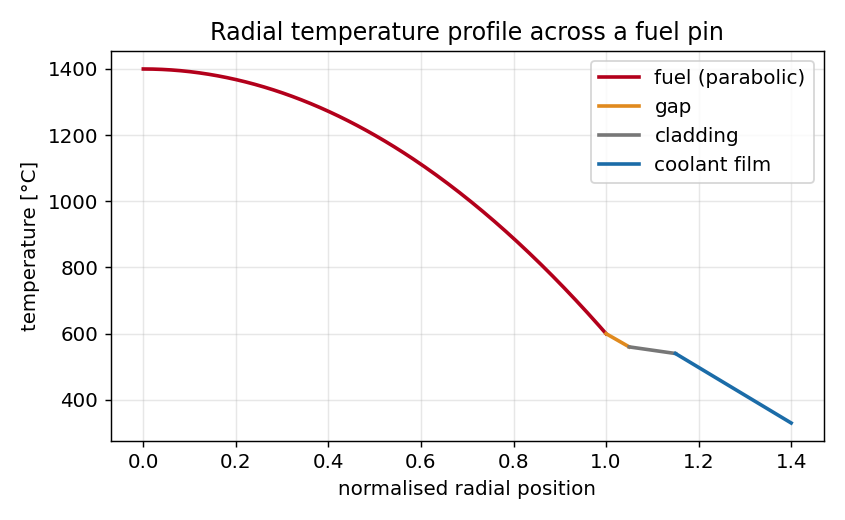
\includegraphics[width=0.74\linewidth]{figures/fuelT.png}
\caption{Schematic radial temperature profile across a fuel pin. The largest drop
is the parabolic profile within the low-conductivity ceramic fuel; further drops
occur across the gap, cladding, and coolant film. The fuel centreline runs
hottest and responds essentially instantly to power changes---the basis of prompt
Doppler feedback.}
\label{fig:fuelT}
\end{figure}

\section{Conduction in the fuel pellet}

For a cylindrical fuel pin with uniform volumetric heat generation $q'''$ and
constant conductivity $k_f$, the steady radial conduction equation
\begin{equation}
\frac{1}{r}\frac{\dd}{\dd r}\!\left(r\,k_f\frac{\dd T}{\dd r}\right) + q''' = 0
\end{equation}
integrates to the parabolic profile
\begin{equation}
T(r) = T_s + \frac{q'''}{4k_f}\!\left(R^2 - r^2\right),
\end{equation}
so the centreline-to-surface temperature rise is
\begin{equation}
\Delta T_{\text{fuel}} = T_c - T_s = \frac{q'''R^2}{4k_f} = \frac{q'}{4\pi k_f},
\end{equation}
where $q'=q'''\pi R^2$ is the linear heat rate (W/m). Remarkably, this rise
depends only on the linear heat rate and the conductivity, not on the pin radius.
Because $\mathrm{UO_2}$ has a low and temperature-dependent conductivity
($k_f$ falls from $\sim 8\unit{W/(m\,K)}$ near room temperature to
$\sim 2\unit{W/(m\,K)}$ at operating temperature), the centreline runs very hot,
often above $1000\degC$ at rated power, even when the surface is near the coolant
temperature. The integral conductivity $\int k_f\,\dd T$ is the natural variable
and is tabulated for fuel design.

\section{Gap, cladding, and film}

Across the pellet--clad gap, heat crosses by conduction through the fill gas and
by radiation; the effective gap conductance $h_g$ depends sensitively on the gap
width, gas composition (helium fill, fission-gas dilution), and burnup. The drop
is $\Delta T_g = q'/(2\pi R\, h_g)$. Conduction through the thin metal cladding
adds a small drop. Finally, convection into the coolant follows Newton's law of
cooling with a heat-transfer coefficient $h$,
\begin{equation}
\Delta T_{\text{film}} = \frac{q'}{2\pi R_{co}\, h},
\end{equation}
where $h$ is obtained from correlations (Dittus--Boelter for single-phase forced
convection; more elaborate correlations in boiling). The total drop from
centreline to bulk coolant is the sum of all four contributions.

\section{The decisive timescales}

For dynamics, the \emph{rates} of temperature change matter as much as the steady
drops. The fuel has a thermal time constant
\begin{equation}
\tau_f = \frac{m_f c_{p,f}}{h_{\text{eff}}A},
\end{equation}
typically a few seconds, after which it equilibrates with the coolant for a given
power. But the \emph{centreline} responds to a power change essentially
instantly---within the conduction time across the pellet---which is why Doppler
feedback (which depends on fuel temperature) is treated as prompt. The coolant
has its own transport time, the time for fluid to traverse the core, of order a
second; moderator and coolant feedback therefore lag the power by this transport
delay. These differing lags---prompt fuel, delayed coolant---are central to
stability: a fast \emph{negative} fuel feedback can stabilise a transient that a
delayed coolant feedback could not catch in time.

\keypoint{The fuel temperature responds promptly to power; the coolant
temperature and void respond with a transport delay. Prompt negative feedback
(Doppler) is the reactor's first and fastest line of defence in a fast
transient; delayed feedback governs the slower stability of the operating point.}

\section{Lumped thermal models for dynamics}

Full thermal-hydraulics is a field in itself, but stability analysis usually uses
\emph{lumped} models that capture the essential dynamics with a few ordinary
differential equations. A widely used two-node model treats the fuel and coolant
as single nodes with temperatures $\Tf$ and $\Tc$:
\begin{align}
m_f c_f \frac{\dd \Tf}{\dd t} &= P(t) - U\!A\,(\Tf - \Tc),\\
m_c c_c \frac{\dd \Tc}{\dd t} &= U\!A\,(\Tf - \Tc) - 2\dot m c_c (\Tc - T_{in}),
\end{align}
where $P$ is the power deposited in the fuel, $U\!A$ the fuel-to-coolant
conductance, $\dot m$ the coolant mass flow, and $T_{in}$ the inlet temperature.
The factor of two in the last term arises from taking the node temperature as the
average of inlet and outlet. Even simpler is the \emph{adiabatic} model used in
fast-excursion analysis, in which heat removal is neglected on the (short)
excursion timescale and the fuel simply integrates the power:
\begin{equation}
C\frac{\dd \Tf}{\dd t} = P(t),
\label{eq:adiabatic}
\end{equation}
with $C$ the fuel heat capacity. This is the model behind the Nordheim--Fuchs
analysis of Chapter~\ref{ch:nonlinear} and the feedback demonstrations of
Chapter~\ref{ch:comp}. Its virtue is that, in the seconds of a prompt excursion,
it is also physically accurate: there simply is not time to remove the heat.

These lumped temperatures are the inputs to the feedback coefficients of the next
chapter. Their dynamics---how fast $\Tf$ and $\Tc$ track power---combine with the
\emph{signs} of the feedback coefficients to determine whether the closed loop is
stable.



\section{Exact conduction in the fuel pin}
\label{sec:fuel-conduction}

\paragraph{Integral conductivity.}
With temperature-dependent $k_f$, define $\theta(T)=\int_{T_{\mathrm{ref}}}^{T}
k_f(T')\dd T'$. Integrating the steady equation
$\frac1r\frac{\dd}{\dd r}(r k_f\,T')+q'''=0$ once gives
$k_f\,\dd T=-(q'''/2)\,r\,\dd r$, hence
\begin{equation}
\theta(T_c)-\theta(T_s)=\frac{q''' R^2}{4}=\frac{q'}{4\pi},
\label{eq:integral-cond}
\end{equation}
\emph{independently of the form of} $k_f(T)$: it is the integral conductivity, not
the temperature, that is linear in the linear heat rate $q'$.

\paragraph{Exact transient solution.}
The homogeneous cylindrical heat equation
$\partial_t T=\kappa(\partial_{rr}T+r^{-1}\partial_r T)$, $\kappa=k_f/(\rho c_p)$,
with $T(R,t)=T_s$, $\partial_rT(0,t)=0$, separates as $T-T_s=\mathcal R(r)e^{-\kappa\nu^2t}$
with $\mathcal R''+\mathcal R'/r+\nu^2\mathcal R=0$, regular solution $J_0(\nu r)$.
The condition $J_0(\nu R)=0$ quantises $\nu_n=\alpha_n/R$ ($J_0(\alpha_n)=0$;
$\alpha_1\approx2.405$), giving
\begin{equation}
T(r,t)-T_s=\sum_{n=1}^{\infty}A_n J_0\!\Big(\frac{\alpha_n r}{R}\Big)
\exp\!\Big(-\frac{\kappa\alpha_n^2}{R^2}t\Big),
\label{eq:bessel-series}
\end{equation}
with $A_n$ from the orthogonality
$\int_0^R J_0(\tfrac{\alpha_n r}{R})J_0(\tfrac{\alpha_m r}{R})r\,\dd r
=\tfrac12 R^2 J_1(\alpha_n)^2\delta_{nm}$.

\begin{proposition}[Fundamental thermal time constant]
\label{prop:thermal-tau}
For $t\gtrsim R^2/\kappa$ the series \eqref{eq:bessel-series} is dominated by $n=1$,
so the fuel relaxes as a single exponential with
\begin{equation}
\tau_f=\frac{R^2}{\kappa\,\alpha_1^2}=\frac{\rho c_p R^2}{k_f\,\alpha_1^2}
\approx\frac{\rho c_p R^2}{5.78\,k_f}.
\end{equation}
\end{proposition}
\begin{proof}
Mode $n$ decays at $\kappa\alpha_n^2/R^2$, increasing in $n$; the ratio of mode $2$
to mode $1$ is $e^{-\kappa(\alpha_2^2-\alpha_1^2)t/R^2}\to0$, leaving the $n=1$
rate $\kappa\alpha_1^2/R^2$, i.e.\ $\tau_f=R^2/(\kappa\alpha_1^2)$,
$\alpha_1^2\approx5.78$.
\end{proof}

\paragraph{The Biot number.}
With $\mathrm{Bi}=hR/k_f$ comparing conduction to convection resistance, the
lumped balance $\rho c_p V\,\dd T/\dd t=-hA(T-T_\infty)$ (decay constant
$\tau=\rho c_p V/(hA)$) is valid for $\mathrm{Bi}\ll1$; for $\mathrm{Bi}\gtrsim1$,
typical of ceramic fuel, the distributed solution \eqref{eq:bessel-series} and
Proposition~\ref{prop:thermal-tau} are required.

\section{Spectral analysis of the two-node thermal model}
\label{sec:twonode-spectral}

Linearising the two-node model about steady state gives $\dot{\boldsymbol\delta}
=\mathbf B\boldsymbol\delta$ for $(\delta\Tf,\delta\Tc)$ with
\begin{equation}
\mathbf B=
\begin{pmatrix}
-\dfrac{U\!A}{m_fc_f} & \dfrac{U\!A}{m_fc_f}\\[6pt]
\dfrac{U\!A}{m_cc_c} & -\dfrac{U\!A+2\dot m c_c}{m_cc_c}
\end{pmatrix}.
\end{equation}
Here $\operatorname{tr}\mathbf B<0$ and
$\det\mathbf B=\dfrac{U\!A\cdot 2\dot m c_c}{m_fc_f\,m_cc_c}>0$, so by the $n=2$
Routh--Hurwitz conditions (Theorem~\ref{thm:rh}) both eigenvalues
\begin{equation}
\lambda_\pm=\tfrac12\Big(\operatorname{tr}\mathbf B\pm
\sqrt{\operatorname{tr}^2\mathbf B-4\det\mathbf B}\Big)
\end{equation}
lie in the left half-plane: the passive thermal network is unconditionally stable.
The constants $\tau_\pm=-1/\lambda_\pm$ are the fast (fuel) and slow (coolant)
lags entering the feedback transfer function $H(s)$ of Chapter~\ref{ch:linear}.
Instability can thus enter only through the neutronic coupling and the sign of the
reactivity feedback, never through the thermal network itself.


\section*{Exercises}
\addcontentsline{toc}{section}{Exercises}
\begin{enumerate}[leftmargin=*,itemsep=2pt]
\item Show that the fuel centreline-to-surface temperature rise depends only on the linear heat rate and conductivity, not the pin radius.
\item List the four temperature drops from fuel centreline to bulk coolant and identify which is usually largest.
\item Explain why Doppler feedback is treated as prompt while moderator feedback is delayed.
\item Justify the adiabatic fuel model \eqref{eq:adiabatic} for analysing a prompt excursion.
\item Estimate the fuel thermal time constant given plausible values and discuss its role in stability.
\end{enumerate}

\chapter{Reactivity Feedback Mechanisms}
\label{ch:feedback}

Feedback is where thermal physics re-enters the neutron economy. This chapter
defines the feedback coefficients, derives the dominant mechanisms---Doppler,
moderator/coolant temperature, and void---and establishes the signs that decide
stability. The void coefficient receives special attention because its sign is
the crux of the Chernobyl story.

\section{Temperature coefficients of reactivity}

A \textbf{temperature coefficient of reactivity} is the change in reactivity per
unit change in some temperature,
\begin{equation}
\alpha_T = \frac{\partial \rho}{\partial T}.
\end{equation}
There is one for each material whose temperature affects the neutron economy:
$\alpha_D=\partial\rho/\partial \Tf$ (the fuel or Doppler coefficient),
$\alpha_M=\partial\rho/\partial T_M$ (the moderator coefficient), and analogously
for coolant and structure. For stability, the sign is paramount: a
\emph{negative} coefficient means that heating removes reactivity, which opposes a
power rise---stabilising. A \emph{positive} coefficient means heating adds
reactivity, reinforcing a power rise---destabilising.

\begin{definition}[Power coefficient]
The \textbf{power coefficient} $\alpha_P=\partial\rho/\partial P$ aggregates all
temperature feedbacks weighted by how strongly each temperature responds to
power:
\begin{equation}
\alpha_P = \alpha_D\frac{\partial \Tf}{\partial P}
         + \alpha_M\frac{\partial T_M}{\partial P}
         + \alpha_v\frac{\partial \bar v}{\partial P} + \cdots
\end{equation}
A negative power coefficient is the single most important guarantee of inherent
stability: it means that any increase in power is self-limiting. Western power
reactors are designed and licensed to have a negative power coefficient across
the operating range.
\end{definition}

\section{The Doppler effect: prompt and reliably negative}

The Doppler coefficient is the reactor's fastest and most dependable feedback. It
arises from the broadening of the neutron-capture resonances of $^{238}$U (and
$^{240}$Pu) as the fuel heats.

At a resonance, the absorption cross-section is sharply peaked at a resonance
energy $E_0$. The thermal motion of the absorbing nuclei---greater at higher
temperature---Doppler-shifts the relative neutron energy, smearing the resonance
into a broader, lower peak while approximately conserving its area
(Figure~\ref{fig:doppler}). The key consequence is that broadening \emph{reduces
self-shielding}: when the resonance is narrow and tall, neutrons at the resonance
energy are absorbed in the thin outer layer of the fuel and the interior is
``shielded''; when the resonance is broadened, more of the fuel volume
participates in absorption. Net resonance absorption therefore \emph{increases}
with temperature, the resonance escape probability $p$ \emph{falls}, and
reactivity \emph{decreases}.

\begin{figure}[H]
\centering
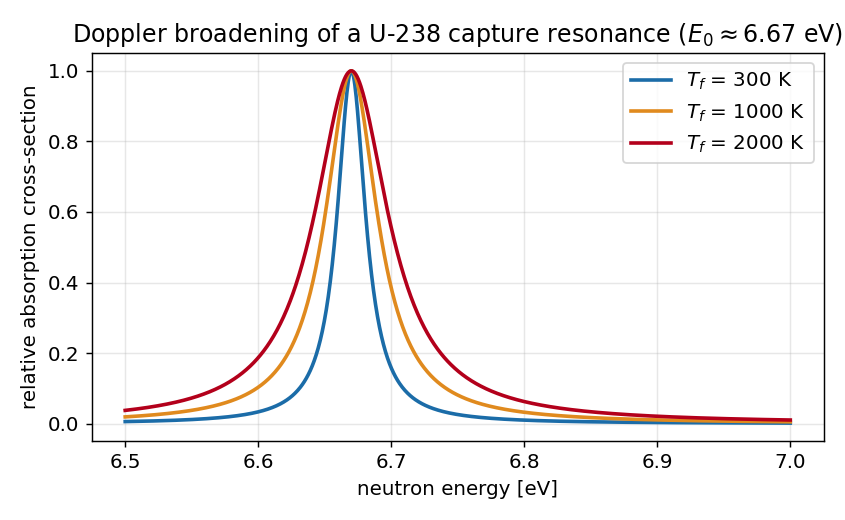
\includegraphics[width=0.74\linewidth]{figures/doppler.png}
\caption{Doppler broadening of a $^{238}$U capture resonance with increasing fuel
temperature. The peak lowers and widens at roughly constant area; reduced
self-shielding increases net resonance absorption, lowering reactivity. This is
the prompt, negative Doppler feedback.}
\label{fig:doppler}
\end{figure}

Two features make Doppler feedback uniquely valuable. First, it is \emph{prompt}:
it depends on the fuel temperature, which rises essentially instantly with power,
so it acts even on a prompt-critical excursion. Second, it is \emph{reliably
negative} in any fuel containing a fertile resonance absorber such as $^{238}$U,
which is to say in essentially all power-reactor fuel. A useful approximate form
is
\begin{equation}
\alpha_D \approx \frac{A}{\sqrt{\Tf}},\qquad
\Delta\rho_D = \int \alpha_D\,\dd \Tf \propto \sqrt{\Tf},
\end{equation}
with $A<0$; the $1/\sqrt{\Tf}$ dependence means the coefficient weakens at high
temperature but never changes sign. It was the absence of a sufficiently strong
\emph{net} prompt negative feedback, not the absence of Doppler per se, that
doomed the RBMK: the RBMK had Doppler feedback, but at low power its huge positive
void coefficient overwhelmed it.

\keypoint{Doppler feedback is prompt and negative. It is the only feedback fast
enough to limit a prompt-critical excursion, and it is the physical reason a
well-designed reactor ``rides out'' a reactivity insertion. The decisive question
for any reactor is whether the prompt feedback is \emph{net} negative once the
void coefficient is included.}

\section{Moderator and coolant temperature feedback}

In a thermal reactor the moderator slows neutrons to thermal energies. Its
temperature affects reactivity through two competing routes: changes in moderator
\emph{density} (a hotter, less dense moderator slows neutrons less effectively),
and changes in the thermal neutron \emph{spectrum} (a hotter moderator hardens
the spectrum, shifting absorption rates). In a light-water reactor the density
effect dominates, and because water is both moderator and coolant, heating it
reduces moderation. Whether this raises or lowers reactivity depends on whether
the lattice is under- or over-moderated:

\begin{itemize}[nosep]
\item In an \textbf{under-moderated} lattice (PWR design intent), there is ``too
little'' moderation at the optimum; reducing it further (by heating/expanding the
water) lowers reactivity. The moderator temperature coefficient (MTC) is
\emph{negative}---stabilising.
\item In an \textbf{over-moderated} lattice, reducing moderation moves toward the
optimum and \emph{raises} reactivity. The MTC is positive---destabilising.
\end{itemize}

Light-water reactors are deliberately designed under-moderated to guarantee a
negative MTC. The moderator coefficient acts with the coolant transport delay
and so governs the slower stability of the operating point rather than the prompt
excursion.

\section{The void coefficient}

When coolant boils (in a BWR, or in any reactor during a transient) or flashes to
steam, it forms \emph{voids}---regions of vapour with much lower density than
liquid. The \textbf{void coefficient} $\alpha_v=\partial\rho/\partial \bar v$,
where $\bar v$ is the void fraction, captures the reactivity effect. Voiding has
several effects at once: it removes moderator (in a water-moderated reactor), it
removes a neutron absorber (water absorbs neutrons), and it changes leakage. The
net sign depends, once again, on whether the lattice is under- or
over-moderated.

\begin{itemize}[nosep]
\item In an \textbf{under-moderated} water reactor (PWR, BWR), the loss of
moderation dominates: voiding lowers reactivity, $\alpha_v<0$---stabilising. A
BWR runs with boiling by design, and its negative void coefficient is the basis
of its self-regulation (and, in fast transients, of a mild instability tendency
discussed in Chapter~\ref{ch:linear}).
\item In the \textbf{RBMK}, moderation was provided primarily by \emph{graphite},
which is unaffected by boiling the water. The water acted mainly as coolant and
as a parasitic \emph{absorber}. Voiding the water therefore removed an absorber
without removing much moderation, so reactivity \emph{rose}: $\alpha_v>0$,
strongly so, and most strongly at low power where the steam fraction was small and
sensitive. This is the single most important design fact behind Chernobyl.
\end{itemize}

\begin{figure}[H]
\centering
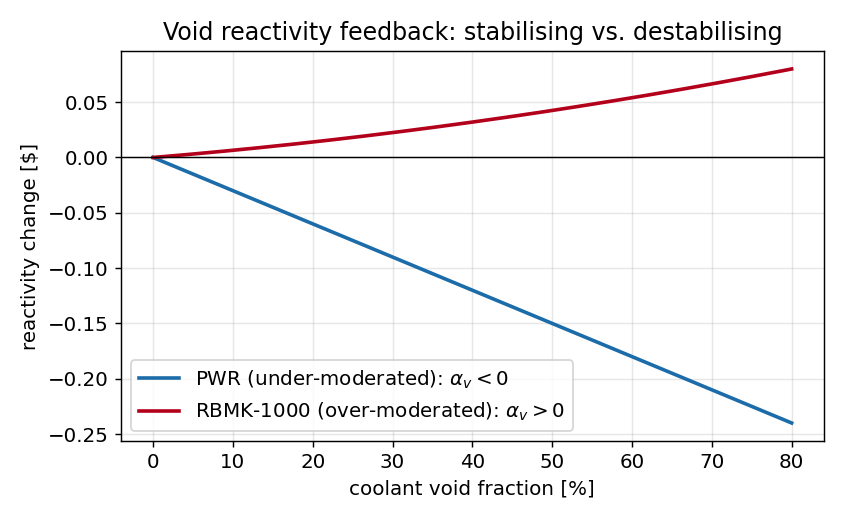
\includegraphics[width=0.74\linewidth]{figures/void.png}
\caption{Void reactivity feedback for an under-moderated lattice (PWR, negative
slope) and an over-moderated lattice (RBMK-1000, positive slope). The void
coefficient is the slope at the operating point; its sign decides whether boiling
is self-limiting or self-amplifying.}
\label{fig:void2}
\end{figure}

\begin{remark}[The vicious circle of a positive void coefficient]
A positive void coefficient creates a runaway loop: power up $\to$ more boiling
$\to$ more voids $\to$ \emph{more} reactivity $\to$ more power. If the prompt
Doppler feedback is not strong enough to overcome it, the loop is unstable. At
the RBMK's low-power, low-flow state on the night of the accident, the loop gain
exceeded unity and the prompt feedback was net positive---a condition the machine
should never have been allowed to enter.
\end{remark}

\section{Other feedbacks: expansion, bowing, and burnup}

Several smaller effects round out the picture. \emph{Thermal expansion} of fuel,
cladding, and structure changes geometry and hence leakage and lattice spacing;
in fast reactors, fuel and structural expansion provide important negative
feedback. \emph{Fuel bowing} and \emph{control-rod-bank expansion} can contribute
small coefficients. Over the long term, \emph{burnup} changes the isotopic
composition and hence all coefficients---a reactor's MTC, for example, becomes
more negative as soluble boron is reduced over a cycle. For the fast dynamics of
stability, however, the trio of Doppler, moderator, and void dominate, and the
contest between prompt-negative Doppler and a possibly-positive void coefficient
is the essential drama.

\section{Assembling the feedback reactivity}

For the coupled model we write the total reactivity as the externally imposed part
plus the feedback,
\begin{equation}
\rho(t) = \rho_{ext}(t)
        + \alpha_D\,[\Tf(t)-\Tf^0]
        + \alpha_M\,[\Tc(t)-\Tc^0]
        + \alpha_v\,[\bar v(t)-\bar v^0] + \cdots
\label{eq:rho-feedback}
\end{equation}
Substituting \eqref{eq:rho-feedback} into the point kinetics
\eqref{eq:prk} and coupling to the thermal equations of
Chapter~\ref{ch:thermal} closes the loop. The resulting nonlinear system is the
subject of Chapter~\ref{ch:coupled} and of the stability analysis of Part~III. Its
behaviour hinges entirely on the signs and magnitudes of the coefficients in
\eqref{eq:rho-feedback}: a system with net-negative, suitably prompt feedback is
stable and self-regulating; a system with net-positive feedback, especially a
prompt one, is an accident waiting for a trigger.



\section{Rigorous theory of the Doppler coefficient}
\label{sec:doppler-rigorous}

We derive the temperature dependence of the Doppler coefficient from
resonance-absorption theory. Near an isolated resonance at $E_0$ the capture
cross-section of a \emph{stationary} target is the Breit--Wigner form
\begin{equation}
\sigma_\gamma^0(E)=\sigma_0\,\frac{\Gamma_\gamma}{\Gamma}\sqrt{\frac{E_0}{E}}\,
\frac{1}{1+x^2},\qquad x=\frac{2(E-E_0)}{\Gamma},
\end{equation}
with total width $\Gamma$, radiative width $\Gamma_\gamma$, and peak $\sigma_0$.
Thermal motion of the target nuclei convolves this with a Maxwellian of relative
velocities, giving the Doppler-broadened shape
\begin{equation}
\sigma_\gamma(E,T)=\sigma_0\,\frac{\Gamma_\gamma}{\Gamma}\sqrt{\frac{E_0}{E}}\,
\psi(\xi,x),\qquad
\psi(\xi,x)=\frac{\xi}{2\sqrt{\pi}}\!\int_{-\infty}^{\infty}\!
\frac{e^{-\frac14\xi^2(x-y)^2}}{1+y^2}\,\dd y,
\label{eq:psi}
\end{equation}
with broadening parameter $\xi=\Gamma/\Delta_D$ and \emph{Doppler width}
\begin{equation}
\Delta_D=\sqrt{\frac{4E_0 k_B T}{A}}\ \propto\ \sqrt{T},
\label{eq:dopplerwidth}
\end{equation}
$A$ the target mass number. The convolution \eqref{eq:psi} conserves area,
$\int_{-\infty}^{\infty}\psi\,\dd x=\pi$, so broadening lowers and widens the line
without changing its integral.

The reactivity effect operates through the \emph{effective resonance integral}
under self-shielding. In the narrow-resonance approximation with background
cross-section $\sigma_b$ per absorber atom,
\begin{equation}
I_{\rm eff}(T)=\int \frac{\sigma_\gamma(E,T)\,\sigma_b}{\sigma_\gamma(E,T)+\sigma_b}\,
\frac{\dd E}{E},
\end{equation}
which is an increasing function of the Doppler width.

\begin{proposition}[Temperature law of the Doppler coefficient]
\label{prop:doppler}
To leading order in the broadening, $\partial I_{\rm eff}/\partial T>0$ with
$\partial I_{\rm eff}/\partial T\propto \dd\Delta_D/\dd T\propto T^{-1/2}$.
Consequently the Doppler coefficient obeys
\begin{equation}
\alpha_D(T)=\frac{\partial\rho}{\partial T}
 =-\frac{1}{p}\,\frac{\partial p}{\partial I_{\rm eff}}\,
   \frac{\partial I_{\rm eff}}{\partial T}
 =\frac{A_D}{\sqrt{T}},\qquad A_D<0,
\end{equation}
so $\alpha_D$ is negative for all $T$ and weakens as $T^{-1/2}$ without ever
changing sign. The reactivity defect $\Delta\rho_D(T)=\int_{T_0}^{T}\alpha_D\,\dd
T'\propto -(\sqrt T-\sqrt{T_0})$ is strictly negative and decreasing.
\end{proposition}
\begin{proof}
Self-shielding makes $I_{\rm eff}$ increase as the line broadens because the
saturated (flat-topped) region of the integrand widens; differentiating the
narrow-resonance integral and using $\partial\Delta_D/\partial T=\tfrac12
\Delta_D/T\propto T^{-1/2}$ from \eqref{eq:dopplerwidth} gives
$\partial I_{\rm eff}/\partial T\propto T^{-1/2}$. Increased resonance capture
lowers the resonance escape probability, $\partial p/\partial I_{\rm eff}<0$, so
$\alpha_D=-p^{-1}(\partial p/\partial I_{\rm eff})(\partial I_{\rm eff}/\partial
T)$ is a negative constant times $T^{-1/2}$. Integrating yields the stated defect.
\end{proof}

Proposition~\ref{prop:doppler} is the rigorous content of the earlier heuristic:
Doppler feedback is prompt (it depends only on $\Tf$), structurally negative (it
needs only a fertile resonance absorber such as $^{238}$U), and bounded below by a
$T^{-1/2}$ law.


\section*{Exercises}
\addcontentsline{toc}{section}{Exercises}
\begin{enumerate}[leftmargin=*,itemsep=2pt]
\item Define the power coefficient and explain why a negative power coefficient guarantees self-limitation.
\item Explain the mechanism by which Doppler broadening reduces self-shielding and lowers reactivity.
\item For an under- and an over-moderated lattice, predict the sign of the void coefficient and justify it.
\item Why is the void coefficient of the RBMK largest at low power?
\item Write the total feedback reactivity \eqref{eq:rho-feedback} and identify which term is prompt.
\end{enumerate}

\chapter{Coupled Neutronic--Thermal-Hydraulic Dynamics}
\label{ch:coupled}

We now assemble the pieces---point kinetics, lumped thermal model, and feedback
coefficients---into a single coupled dynamical system and explore its qualitative
behaviour before the formal stability analysis of Part~III.

\section{The closed-loop model}

Combining the point kinetics \eqref{eq:prk}, the lumped thermal model of
Chapter~\ref{ch:thermal}, and the feedback law \eqref{eq:rho-feedback}, a compact
representative model is
\begin{align}
\frac{\dd p}{\dd t} &= \frac{\rho(t)-\beta}{\Lambda}\,p + \sum_i \lambda_i \zeta_i,\\
\frac{\dd \zeta_i}{\dd t} &= \frac{\beta_i}{\Lambda}\,p - \lambda_i \zeta_i,\\
C_f\frac{\dd \Tf}{\dd t} &= P_0\,p - U\!A\,(\Tf-\Tc),\\
C_c\frac{\dd \Tc}{\dd t} &= U\!A\,(\Tf-\Tc) - 2\dot m c_c(\Tc-T_{in}),\\
\rho(t) &= \rho_{ext}(t) + \alpha_D(\Tf-\Tf^0) + \alpha_c(\Tc-\Tc^0).
\end{align}
This is a system of nonlinear ordinary differential equations: nonlinear because
reactivity multiplies power in the first equation, and reactivity itself depends
on the temperatures driven by power. The nonlinearity is essential---it is what
makes a power excursion turn over rather than grow forever---but it also makes the
behaviour rich.

\section{The self-regulating reactor in words}

Before any mathematics, the qualitative behaviour of a \emph{negative-feedback}
reactor is worth stating plainly. Suppose the operator withdraws a control rod,
inserting positive $\rho_{ext}$. Power rises. The fuel heats within milliseconds;
if $\alpha_D<0$, this immediately subtracts reactivity, blunting the rise. As the
coolant heats over the next second, $\alpha_c<0$ subtracts more. The reactor
settles at a higher power and temperature at which the feedback exactly cancels
the inserted reactivity: a new stable operating point. The reactor has
\emph{regulated itself} without any control action. Conversely, if the operator
reduces power, temperatures fall, feedback adds reactivity, and the fall is
arrested. This is the everyday meaning of a negative power coefficient.

Now reverse the sign of the dominant feedback, as in the RBMK at low power. The
rod withdrawal raises power; boiling increases; the positive void coefficient
adds \emph{more} reactivity; power rises further; and unless a strong prompt
negative effect intervenes, the excursion accelerates. The same control action
that a stable reactor absorbs, the unstable one amplifies.

\section{Equilibrium and the power defect}

At equilibrium the time derivatives vanish and the feedback exactly offsets the
external reactivity. The total reactivity that must be supplied by control to
hold the reactor critical from cold-zero-power to hot-full-power is the
\textbf{power defect},
\begin{equation}
\Delta\rho_{\text{defect}} = -\!\int_0^{P_0}\!\alpha_P\,\dd P,
\end{equation}
which for a negative power coefficient is positive (control must \emph{add}
reactivity to reach full power, because the feedback removes it). The power defect
is a useful integral measure of how strongly self-regulating a reactor is, and it
must be matched by available control-rod and chemical-shim worth.

\section{Linearisation preview}

For small perturbations about an operating point, write $p=p_0+\delta p$,
$\Tf=\Tf^0+\delta \Tf$, etc., and keep first-order terms. The linearised system
has the form $\dot{\mathbf x}=\mathbf A\,\mathbf x + \mathbf b\,\rho_{ext}$, and
its stability is decided by the eigenvalues of the matrix $\mathbf A$: the
operating point is stable if and only if all eigenvalues have negative real part.
The feedback coefficients enter $\mathbf A$ directly, so the sign and magnitude of
$\alpha_D$, $\alpha_c$, and $\alpha_v$ determine the eigenvalues' signs. This is
the formal content of Chapter~\ref{ch:linear}, where we also pass to the frequency
domain and the Nyquist criterion, which handles the transport delays more
naturally than eigenvalues alone.

\section{A demonstration of self-limitation}

Figure~\ref{fig:transients} (bottom right) already showed the canonical result:
a reactivity-initiated excursion that, with negative feedback, rises to a peak and
then turns over as the heating fuel removes reactivity. The peak power, the time
to peak, and the total energy released are set by the competition between the
inserted reactivity and the feedback strength---precisely the Nordheim--Fuchs
balance derived in Chapter~\ref{ch:nonlinear}. The same model with the feedback
sign flipped does not turn over; it diverges until the model's assumptions break.
The entire safety case of an inherently stable reactor rests on getting that sign
right and the magnitude large enough.

\keypoint{The coupled model is nonlinear, but its stability is governed by a
simple principle: the feedback must remove reactivity as power and temperature
rise, and it must do so promptly enough. Part~III makes ``promptly enough''
precise through eigenvalues and the Nyquist criterion; Part~IV shows what the
violation of this principle looked like in practice.}


\section*{Exercises}
\addcontentsline{toc}{section}{Exercises}
\begin{enumerate}[leftmargin=*,itemsep=2pt]
\item Describe in words the self-regulating response of a negative-feedback reactor to a rod withdrawal.
\item Define the power defect and explain its sign for a negative power coefficient.
\item Explain how the feedback coefficients enter the linearised system matrix and why feedback is more potent at higher power.
\item Sketch the qualitative power response of a reactor with positive feedback to a small rod withdrawal.
\item Why does a nonlinear feedback model produce a power excursion that turns over, while a linear analysis cannot capture the turnover?
\end{enumerate}


\part{Stability Theory}
\chapter{Linear Stability and Frequency-Domain Methods}
\label{ch:linear}

Stability is, in the first instance, a question about \emph{small} perturbations:
does a tiny disturbance grow or decay? This is the domain of linear stability
analysis. We linearise the coupled model, introduce the zero-power and
feedback transfer functions, and apply the Nyquist criterion, which handles the
transport delays of real reactors more gracefully than eigenvalues alone.

\section{Linearisation about an operating point}

Let the reactor sit at steady power $p_0$ with steady temperatures, and perturb:
$p=p_0+\delta p$, $\zeta_i=\zeta_{i0}+\delta\zeta_i$, $\Tf=\Tf^0+\delta\Tf$, and
so on. Substituting into the coupled equations of Chapter~\ref{ch:coupled} and
discarding products of small quantities gives a linear system
\begin{equation}
\frac{\dd}{\dd t}\,\delta\mathbf{x} = \mathbf{A}\,\delta\mathbf{x}
   + \mathbf{b}\,\delta\rho_{ext},
\end{equation}
where $\delta\mathbf{x}=(\delta p,\delta\zeta_1,\dots,\delta\zeta_6,
\delta\Tf,\delta\Tc)^{\!\top}$. The crucial linearised coupling is in the power
equation: the term $(\rho-\beta)p/\Lambda$ contributes
$p_0\,\delta\rho/\Lambda$, and $\delta\rho = \alpha_D\,\delta\Tf +
\alpha_c\,\delta\Tc$. Thus the feedback coefficients enter $\mathbf A$ multiplied
by $p_0/\Lambda$: \emph{feedback is more potent at higher power}, an observation
with direct bearing on why the RBMK was most dangerous at low power.

The operating point is asymptotically stable if and only if every eigenvalue of
$\mathbf A$ has negative real part. For the bare point-kinetics block (no
feedback) the eigenvalues are exactly the inhour roots of
Chapter~\ref{ch:pk}; adding negative feedback pushes the dominant root further
into the left half-plane (more stable), while positive feedback pulls it toward,
and possibly across, the imaginary axis (instability).

\section{The zero-power transfer function}

Frequency-domain analysis is more illuminating for systems with delays. Laplace
transform the point kinetics about $p_0$ with input $\delta\rho$ and output
$\delta p/p_0$; eliminating the precursors gives the \textbf{zero-power reactor
transfer function}
\begin{equation}
Z(s) = \frac{\delta p/p_0}{\delta\rho}
     = \frac{1}{\,\Lambda s + \displaystyle\sum_{i}\frac{\beta_i s}{s+\lambda_i}\,}.
\label{eq:zpr}
\end{equation}
Its denominator is exactly the inhour function \eqref{eq:inhour}; its poles are
the inhour roots. The name ``zero-power'' signals that no thermal feedback is
included: it is the open-loop response of the neutronics alone. At low frequency
$Z(s)$ behaves like an integrator with a long effective time constant set by the
precursors; at high frequency $Z(s)\to 1/(\Lambda s)$, the fast prompt response.
The transition between these regimes, around the delayed-neutron frequencies, is
where the reactor's dynamic character lives.

\section{Closing the loop: the feedback transfer function}

Let the feedback path have transfer function $H(s)$ relating a power perturbation
to the feedback reactivity it produces, $\delta\rho_{fb}=-H(s)\,\delta p/p_0$
(the minus sign for negative feedback). For a single lumped fuel node with
coefficient $\alpha_D<0$ and thermal time constant $\tau_f$,
\begin{equation}
H(s) = \frac{|\alpha_D|\,K}{1+\tau_f s},
\end{equation}
a first-order lag: fast feedback at low frequency, attenuated and phase-lagged at
high frequency. The closed-loop transfer function from external reactivity to
power is
\begin{equation}
G(s) = \frac{Z(s)}{1 + Z(s)H(s)},
\end{equation}
and stability is governed by the roots of the characteristic equation
$1+Z(s)H(s)=0$. The product $Z(s)H(s)$ is the \emph{open-loop gain}; everything
hinges on its behaviour.

\section{The Nyquist criterion}

The Nyquist criterion reads stability directly off a plot of the open-loop gain
$Z(j\omega)H(j\omega)$ as $\omega$ runs over all frequencies. The closed loop is
stable provided the Nyquist locus does not encircle the critical point $-1$ in the
complex plane. Physically, encirclement of $-1$ means there is a frequency at
which the feedback, after its phase lag, returns \emph{in phase} with the
disturbance and with gain exceeding unity---positive feedback at that frequency,
hence growth.

This is where \emph{phase lag} becomes dangerous even for nominally negative
feedback. If the feedback is negative at zero frequency but accumulates enough
phase lag (from thermal transport delays, coolant transit, etc.) that at some
frequency it is delayed by half a cycle, it acts as \emph{positive} feedback at
that frequency. If the loop gain there exceeds one, the reactor oscillates with
growing amplitude. Boiling-water reactors, with their void feedback transported
by the coolant, are the classic example: they can exhibit lightly damped or even
growing power--flow oscillations under certain low-flow, high-power conditions,
and operating limits are drawn specifically to keep the decay ratio safely below
one.

\begin{definition}[Decay ratio]
The decay ratio is the ratio of the amplitudes of two successive peaks of an
oscillatory response to a perturbation. A decay ratio below $1$ indicates a
damped, stable response; equal to $1$ marks the stability boundary; above $1$ the
oscillation grows. BWR stability is monitored and licensed in these terms,
typically with a limit well below unity.
\end{definition}

\section{Gain and phase margins}

The robustness of stability is quantified by the \emph{gain margin} (how much the
loop gain could increase before the locus reaches $-1$) and the \emph{phase
margin} (how much additional phase lag could be tolerated). A reactor designed for
inherent stability carries comfortable margins so that variations over the fuel
cycle, across power levels, and under off-normal conditions never erode stability.
The RBMK at low power had, in effect, negative margins in the relevant
configuration: its dominant feedback was positive, so no amount of phase
bookkeeping could save it---the locus enclosed $-1$ outright.

\section{Power dependence and the low-power trap}

Because feedback enters the loop gain multiplied by $p_0$, a reactor's stability
character changes with power. A \emph{positive}-feedback reactor like the RBMK is
most unstable at \emph{low} power: there the steam void fraction is small and most
sensitive, so the void coefficient is largest, while the prompt Doppler feedback
(which scales with the fuel-temperature changes that low power barely produces) is
weakest. The result is a window of operation---low power, high positive void
worth, depleted control margin---in which the machine is acutely unstable. The
Chernobyl test drove the reactor straight into that window.

\keypoint{Linear stability is decided by the eigenvalues of the linearised
system, or equivalently by whether the Nyquist locus of the open-loop gain
$Z(s)H(s)$ encircles $-1$. Negative feedback with small phase lag keeps the locus
clear; positive feedback, or negative feedback with excessive transport lag, can
enclose $-1$ and produce growing oscillations or divergence. Stability margins
must hold across all power levels and cycle conditions---a requirement the RBMK
violated at low power.}



\section{State-space form and the Routh--Hurwitz criterion}
\label{sec:statespace}

To make ``stability'' fully explicit, reduce to the one-precursor,
one-temperature model that retains the essential feedback physics:
\begin{equation}
\dot n=\frac{\rho-\beta}{\Lambda}n+\lambda C,\quad
\dot C=\frac{\beta}{\Lambda}n-\lambda C,\quad
\dot T=\frac{n}{\mu}-\theta T,\quad \rho=\rho_0+\alpha T,
\end{equation}
with heat capacity $\mu>0$, cooling rate $\theta>0$, and feedback coefficient
$\alpha$. Linearising about the critical equilibrium $(n_0,C_0,T_0)$ with
$\rho_0=0$ gives the Jacobian
\begin{equation}
\mathbf A=
\begin{pmatrix}
-\dfrac{\beta}{\Lambda} & \lambda & \dfrac{\alpha n_0}{\Lambda}\\[5pt]
\dfrac{\beta}{\Lambda} & -\lambda & 0\\[5pt]
\dfrac{1}{\mu} & 0 & -\theta
\end{pmatrix},
\end{equation}
whose characteristic polynomial is $\det(s\mathbf I-\mathbf A)=s^3+a_1s^2+a_2s+a_3$
with
\begin{equation}
a_1=\lambda+\theta+\frac{\beta}{\Lambda},\quad
a_2=\theta\Big(\lambda+\frac{\beta}{\Lambda}\Big)-\frac{\alpha n_0}{\Lambda\mu},\quad
a_3=-\frac{\alpha n_0\lambda}{\Lambda\mu}.
\label{eq:rh-coeffs}
\end{equation}

\begin{theorem}[Routh--Hurwitz, cubic]
\label{thm:rh}
The polynomial $s^3+a_1s^2+a_2s+a_3$ (real coefficients) has all roots in the open
left half-plane if and only if $a_1>0$, $a_3>0$, and $a_1a_2>a_3$.
\end{theorem}

\begin{proposition}[Feedback sign decides stability]
\label{prop:stab}
With $\lambda,\theta,\beta,\Lambda,\mu,n_0>0$, the equilibrium is asymptotically
stable if and only if $\alpha<0$.
\end{proposition}
\begin{proof}
By \eqref{eq:rh-coeffs}, $a_1>0$ always. Now $a_3=-\alpha n_0\lambda/(\Lambda\mu)$,
so $a_3>0\iff\alpha<0$. If $\alpha<0$ then also $a_2=\theta(\lambda+\beta/\Lambda)
+|\alpha|n_0/(\Lambda\mu)>0$, and
\[
a_1a_2-a_3
=\underbrace{(\lambda+\theta+\tfrac{\beta}{\Lambda})\,\theta(\lambda+\tfrac{\beta}{\Lambda})}_{>0}
+\frac{|\alpha|n_0}{\Lambda\mu}\Big[(\lambda+\theta+\tfrac{\beta}{\Lambda})-\lambda\Big]
=(\cdots)+\frac{|\alpha|n_0}{\Lambda\mu}\Big(\theta+\tfrac{\beta}{\Lambda}\Big)>0,
\]
so all three Routh--Hurwitz conditions of Theorem~\ref{thm:rh} hold and the
equilibrium is asymptotically stable. Conversely, if $\alpha>0$ then $a_3<0$,
violating the necessary condition $a_3>0$, so at least one root lies in the closed
right half-plane and the equilibrium is unstable. ($\alpha=0$ is the neutral case,
$a_3=0$, with a root at the origin.)
\end{proof}

Proposition~\ref{prop:stab} is the precise version of the book's thesis: with all
thermal and kinetic parameters positive, \emph{the sign of the feedback
coefficient alone} decides linear stability. The RBMK's low-power state had the
effective $\alpha>0$ and was therefore linearly unstable.

\paragraph{Lyapunov viewpoint.}
By Theorem~\ref{thm:lyap} (Appendix~\ref{app:math}), $\alpha<0$ guarantees a
quadratic Lyapunov function $V(\mathbf x)=\mathbf x^{\!\top}\mathbf P\mathbf x$ with
$\mathbf P\succ0$ solving $\mathbf A^{\!\top}\mathbf P+\mathbf P\mathbf A=-\mathbf
Q$ for any $\mathbf Q\succ0$; then $\dot V=-\mathbf x^{\!\top}\mathbf Q\mathbf x<0$
certifies decay of every small perturbation. Stability is thus not merely
spectral but energy-dissipative.

\section{The Nyquist criterion, precisely}
\label{sec:nyquist-precise}

For the full delayed system the loop gain $L(s)=Z(s)H(s)$ is meromorphic, and
stability is read off by the argument principle.

\begin{theorem}[Nyquist]
\label{thm:nyquist}
Let $L(s)$ be the open-loop transfer function with $P$ poles in the open right
half-plane. As $s$ traverses the Nyquist contour (the imaginary axis closed by an
infinite right semicircle), let $N$ be the number of clockwise encirclements of
the point $-1$ by $L(s)$. Then the number of closed-loop poles in the right
half-plane is $Z=N+P$. The closed loop is stable iff $Z=0$, i.e.\ iff
$N=-P$.
\end{theorem}
\begin{proof}[Sketch]
Closed-loop poles are zeros of $1+L(s)$. By the argument principle, as $s$ runs
over the closed contour, the net change in $\arg(1+L(s))$ equals $2\pi(Z-P)$,
where $Z,P$ count zeros and poles of $1+L$ (equivalently poles of $L$) inside the
contour. The change in $\arg(1+L)$ is $2\pi$ times the clockwise encirclements of
the origin by $1+L$, i.e.\ of $-1$ by $L$; hence $N=Z-P$.
\end{proof}

For an open-loop-stable reactor ($P=0$) the criterion reduces to the familiar
statement: stability iff the locus $L(j\omega)$ does not encircle $-1$. Phase lag
in $H(s)$ from thermal transport can rotate the locus until it encircles $-1$,
which is the frequency-domain face of Proposition~\ref{prop:stab}'s sign change.


\section*{Exercises}
\addcontentsline{toc}{section}{Exercises}
\begin{enumerate}[leftmargin=*,itemsep=2pt]
\item Write the zero-power transfer function \eqref{eq:zpr} and identify its poles.
\item State the Nyquist stability criterion and interpret encirclement of $-1$ physically.
\item Explain how phase lag can turn nominally negative feedback into destabilising feedback at some frequency.
\item Define the decay ratio and state the stability condition in terms of it.
\item Explain why a positive-feedback reactor is most unstable at low power.
\end{enumerate}

\chapter{Nonlinear Power Excursions}
\label{ch:nonlinear}

Linear analysis tells us whether an operating point is stable. When a reactor is
driven hard---a large, fast reactivity insertion---the response is fully
nonlinear, and the question becomes: how high does the power spike, how much
energy is deposited, and what stops it? The classic answer is the
Nordheim--Fuchs model, which gives a remarkably clean closed-form description of a
self-limiting prompt excursion. This is the model that quantifies what a
\emph{thermally stable} reactor does when subjected to a reactivity-initiated
accident---and, by its failure, what Chernobyl did.

\section{The reactivity-initiated accident}

A reactivity-initiated accident (RIA) is a rapid insertion of positive
reactivity---an ejected control rod, a cold-water slug, or, at Chernobyl, the
catastrophic positive scram. If the insertion exceeds one dollar, the reactor
becomes prompt-critical and the power rises on the $\Lambda$ timescale, far too
fast for delayed neutrons or mechanical systems to matter. The only thing that can
arrest it is prompt feedback. Whether the excursion is a benign, self-terminating
spike or an explosive energy release depends entirely on the sign and strength of
that prompt feedback.

\section{The Nordheim--Fuchs model}

Consider a step insertion $\rho_0>\beta$ on a prompt-critical reactor with prompt
negative feedback. On the prompt timescale the delayed neutrons are a nearly
constant background, so we drop the precursor term and write the prompt kinetics
\begin{equation}
\frac{\dd p}{\dd t} = \frac{\rho(t)-\beta}{\Lambda}\,p,
\end{equation}
with feedback through an adiabatically heating fuel (Chapter~\ref{ch:thermal}),
\begin{equation}
\rho(t) = \rho_0 - \gamma\,\big(E(t)\big),\qquad
\frac{\dd E}{\dd t} = p,
\end{equation}
where $E(t)=\int_0^t p\,\dd t'$ is the energy released and $\gamma>0$ is the
magnitude of the (negative) feedback per unit energy---the product of the fuel
heat capacity and the temperature coefficient, $\gamma=|\alpha|/C$. Writing the
prompt reactivity above critical as $\rho_0-\beta$ and feedback $-\gamma E$, the
power is
\begin{equation}
\frac{\dd p}{\dd t} = \frac{(\rho_0-\beta) - \gamma E}{\Lambda}\,p.
\end{equation}
Using $\dd p/\dd t = (\dd p/\dd E)\,p$ and integrating once,
\begin{equation}
p(E) = p_0 + \frac{1}{\Lambda}\!\left[(\rho_0-\beta)E - \tfrac12\gamma E^2\right].
\end{equation}

\section{Peak power, energy, and temperature rise}

The power peaks when $\dd p/\dd t=0$, i.e.\ when the feedback exactly cancels the
prompt reactivity, $\gamma E_{\text{peak}} = \rho_0-\beta$, so the energy released
at the peak is
\begin{equation}
\boxed{\ E_{\text{peak}} = \frac{\rho_0-\beta}{\gamma}\ }
\end{equation}
The excursion does not stop here---the power is maximal, not zero---but the
feedback now drives the reactivity below prompt-critical and the power falls. The
total energy released as the prompt spike completes is, by the symmetry of the
parabola $p(E)$, twice the energy at the peak:
\begin{equation}
\boxed{\ E_{\text{total}} \approx \frac{2(\rho_0-\beta)}{\gamma}\ }
\end{equation}
and the peak power is
\begin{equation}
p_{\max} \approx \frac{(\rho_0-\beta)^2}{2\gamma\Lambda}.
\end{equation}
The corresponding adiabatic fuel temperature rise is
$\Delta \Tf = E_{\text{total}}/C = 2(\rho_0-\beta)/(\gamma C)$. These formulae are
the quantitative essence of self-limitation: the stronger the negative feedback
$\gamma$, the smaller the energy release and temperature rise; the larger the
prompt reactivity excess $\rho_0-\beta$, the larger and sharper the spike.

\begin{example}[A benign spike vs.\ a destructive one]
With prompt feedback strong enough that $\gamma$ limits $\Delta \Tf$ to a few
hundred kelvin, an RIA produces a fast spike that the fuel survives---this is the
designed-for behaviour validated in tests such as SPERT and BORAX. If instead the
\emph{net} prompt feedback is weak, near zero, or---catastrophically---positive,
$E_{\text{total}}$ grows without the parabolic turnover, the temperature rise is
unbounded in the model, and in reality the energy deposition fragments the fuel,
flashes the coolant, and disassembles the core. Chernobyl's excursion deposited
enough energy in a fraction of a second to shatter the fuel and trigger a steam
explosion, precisely because the prompt feedback in its configuration was not
saving-ly negative.
\end{example}

\section{Self-disassembly and the ultimate shutdown}

In the most violent excursions a second, brutal feedback eventually intervenes:
the core physically disassembles. Thermal expansion, fuel vaporisation, and
pressure-driven dispersal increase neutron leakage and separate the fissile
material, terminating the chain reaction---the Fuchs--Hansen ``disassembly''
mechanism that ended the historical criticality excursions (SL-1, the Godiva and
SPERT destructive tests). Disassembly is a shutdown mechanism only in the sense
that an explosion ends a chain reaction: it does so by destroying the reactor. The
purpose of thermal stability and prompt negative feedback is to terminate the
excursion by gentle means---temperature feedback---long before disassembly is
reached.

\section{Connection to the linear picture}

The Nordheim--Fuchs excursion and the linear stability of Chapter~\ref{ch:linear}
are two limits of the same coupled system. Linear analysis governs small
perturbations about an operating point and asks whether they grow; the
Nordheim--Fuchs analysis governs the large, fast, prompt-critical transient and
asks how the nonlinear feedback caps it. A reactor that is linearly stable with
strong negative feedback is also the one whose Nordheim--Fuchs excursions are
mild. A reactor that is linearly unstable---positive feedback---has no benign
nonlinear limit; its excursions terminate only by disassembly. The companion
computations of Chapter~\ref{ch:comp} show both behaviours side by side.

\keypoint{In a prompt-critical excursion, prompt negative feedback caps the energy
release at $E_{\text{total}}\approx 2(\rho_0-\beta)/\gamma$ and the reactor
survives. Without net negative prompt feedback there is no such cap, and the
excursion ends only by destroying the core. Thermal stability is the difference
between a spike and an explosion.}


\section*{Exercises}
\addcontentsline{toc}{section}{Exercises}
\begin{enumerate}[leftmargin=*,itemsep=2pt]
\item Derive $E_{\text{peak}}=(\rho_0-\beta)/\gamma$ from the Nordheim--Fuchs model.
\item Show that the total energy release is approximately $2(\rho_0-\beta)/\gamma$.
\item How does the peak power scale with the prompt reactivity excess and the feedback strength?
\item What physically terminates an excursion when prompt feedback is absent?
\item Relate the sign of the feedback in the Nordheim--Fuchs model to the linear stability of Chapter 8.
\end{enumerate}

\chapter{Xenon Dynamics and Spatial Instability}
\label{ch:xenon}

Not all instabilities are fast. The slowest and most insidious arise from
$^{135}$Xe, a fission product with an enormous neutron-absorption cross-section
whose concentration lags the power by hours. Xenon dynamics produce the
post-shutdown ``dead time'' that constrains operation, and---in large cores---slow
spatial power oscillations. Both played a direct role at Chernobyl: it was xenon
poisoning, following an unplanned power drop, that lured the operators into
withdrawing nearly all the control rods, stripping the reactor of the shutdown
margin that might have saved it.

\section{The iodine--xenon chain}

$^{135}$Xe is produced in two ways: directly from fission (a small yield) and,
dominantly, from the beta-decay of its precursor $^{135}$I (half-life
$\sim 6.6\unit{h}$), which is itself a fission product (yield $\gamma_I\approx
6.4\%$). $^{135}$Xe is destroyed in two ways: by its own beta-decay (half-life
$\sim 9.2\unit{h}$) and by neutron capture---``burnup''---into $^{136}$Xe. Its
thermal absorption cross-section is about $2.6\times10^{6}\unit{barn}$, among the
largest known, so even trace amounts poison the reactor. The governing equations
are
\begin{align}
\frac{\dd I}{\dd t} &= \gamma_I \Sigma_f \phi - \lambda_I I,\\
\frac{\dd X}{\dd t} &= \gamma_X \Sigma_f \phi + \lambda_I I
                       - \lambda_X X - \sigma_X^a \phi\, X,
\end{align}
where $I$ and $X$ are the iodine and xenon concentrations, $\phi$ the flux, and
$\sigma_X^a$ the xenon absorption cross-section. The xenon contributes a negative
reactivity $\rho_X \propto -\sigma_X^a X$.

\section{Equilibrium xenon and its flux dependence}

At steady flux the concentrations reach equilibrium,
\begin{equation}
I_\infty = \frac{\gamma_I\Sigma_f\phi}{\lambda_I},\qquad
X_\infty = \frac{(\gamma_I+\gamma_X)\Sigma_f\phi}{\lambda_X + \sigma_X^a\phi}.
\end{equation}
At high flux, $\sigma_X^a\phi \gg \lambda_X$ and $X_\infty$ saturates: burnup
removes xenon as fast as it is made. The equilibrium xenon reactivity worth in a
high-power thermal reactor is large, of order a few per cent $\Delta k$---several
dollars---which must be compensated by control. The crucial nonlinearity is that
production of xenon (via iodine) depends on the \emph{past} flux, while burnup
depends on the \emph{present} flux; this time mismatch is the engine of every
xenon transient.

\section{The post-shutdown xenon peak and dead time}

Suppose the reactor is shut down (or its power sharply reduced) from a high flux.
Burnup of xenon ($\sigma_X^a\phi X$) stops immediately because $\phi$ collapses,
but the stockpiled iodine keeps decaying into xenon for hours. The xenon
concentration therefore \emph{rises} after shutdown, peaking several hours later
before the slower xenon decay finally wins and it falls. This transient buildup
adds a large negative reactivity---the ``xenon peak'' or ``iodine pit.'' If the
reactor's excess reactivity is insufficient to override the peak, it cannot be
restarted until the xenon decays: the \textbf{xenon dead time}, typically many
hours. Operators must either restart promptly (before the peak) or wait it out.

\begin{remark}[Chernobyl and the xenon trap]
On the night of 25--26 April 1986, the Chernobyl test was delayed and the reactor
power was held low and then dropped far below plan---down to about $30\unit{MW}$
thermal---for an extended period. Xenon built up and poisoned the core. To raise
power against the xenon, operators withdrew control rods far beyond the permitted
operating reactivity margin. The reactor was thus held critical only by a
dangerously small number of inserted rods, with most absorbers removed---a
configuration in which both the shutdown capability and the void coefficient were
at their worst. Xenon dynamics did not cause the explosion, but they set the
trap.
\end{remark}

\section{Spatial xenon oscillations}

In a physically large core---and the RBMK was very large, about $12\unit{m}$ in
diameter---the point approximation fails for slow phenomena, and xenon can drive
\emph{spatial} oscillations even at constant total power. The mechanism is a
delayed, out-of-phase feedback between flux and xenon:

\begin{enumerate}[nosep]
\item A perturbation raises the flux in one region (say, the top of the core) and
lowers it in another (the bottom).
\item In the high-flux region, xenon \emph{burns out} faster than it is produced,
so its concentration falls, which \emph{raises} the local reactivity and pushes
the flux even higher.
\item Meanwhile the extra iodine produced earlier in that region decays into
xenon hours later, eventually \emph{raising} the xenon and suppressing the flux
there---just as the other region, now iodine-rich, begins to flare.
\item The high-flux and low-flux regions thus trade places with a period of
roughly $15\!-\!30\unit{h}$.
\end{enumerate}

\begin{figure}[H]
\centering
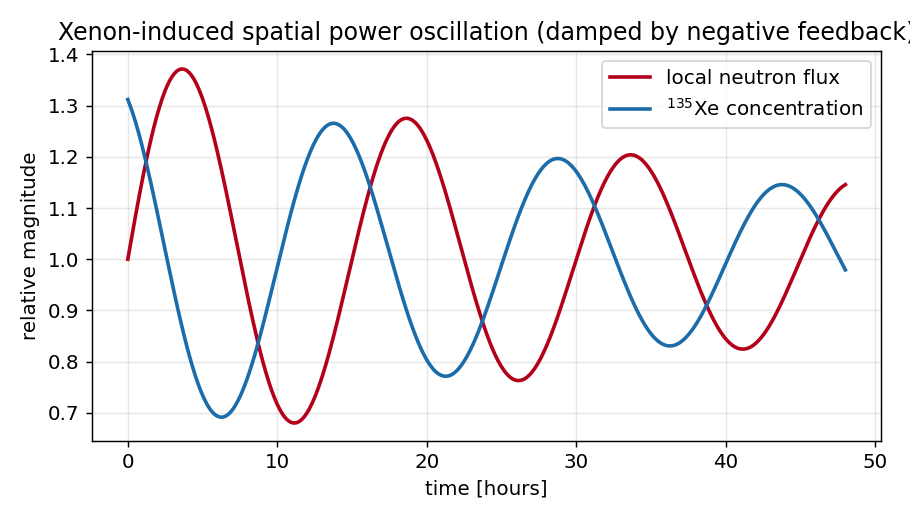
\includegraphics[width=0.82\linewidth]{figures/xenon.png}
\caption{Xenon-induced spatial power oscillation. The local flux and the
$^{135}$Xe concentration oscillate out of phase with a period of order a day. A
sufficiently negative power (temperature) coefficient damps the oscillation;
without it, the amplitude can grow.}
\label{fig:xenon}
\end{figure}

Whether these oscillations grow or decay depends on the power coefficient. A
strong \emph{negative} temperature/power coefficient damps them: as a region's
power rises, its temperature rises and removes reactivity, opposing the xenon-led
growth. A weak or positive coefficient leaves the oscillation undamped or growing.
Large reactors counter spatial xenon instability with negative feedback and with
spatial control (segmented control rods, flux mapping, and active power-shaping).
The RBMK required constant operator attention to its axial and radial power
distribution precisely because of its size and its marginal feedback; the night of
the accident, the flux shape was badly distorted (axially peaked), worsening the
local void and power coefficients beyond what core-average figures suggested.

\section{Implications for stability and operation}

Xenon dynamics teach two lessons relevant to thermal stability. First, the
reactor's state depends on its \emph{history}: the same power level can correspond
to very different xenon (and hence reactivity and rod) configurations depending on
what the power did over the preceding day. Operating procedures must account for
this memory. Second, spatial effects mean that a core can be ``stable on
average'' yet locally unstable; core-average coefficients can mislead. Both
lessons were violated at Chernobyl, where a history of power manoeuvring produced a
xenon-poisoned, rod-depleted, axially-distorted core whose local stability was far
worse than any single average number would suggest.

\keypoint{Xenon-135 introduces hours-long memory into reactor dynamics: a
post-shutdown poisoning peak that can preclude restart, and---in large cores---slow
spatial power oscillations damped only by negative feedback. At Chernobyl, xenon
poisoning drove the operators to strip out the control rods, creating the
low-margin, distorted-flux state in which the positive void coefficient could
trigger catastrophe.}



\section{Linear stability of the iodine--xenon equilibrium}
\label{sec:xenon-stability}

We now analyse xenon dynamics rigorously, first at a point (temporal stability)
and then for a spatial mode (the oscillation).

\paragraph{Temporal stability at fixed flux.}
Linearise the iodine--xenon equations about the equilibrium $(I_\infty,X_\infty)$
at constant flux $\phi_0$. With state $(\delta I,\delta X)$ the Jacobian is
\begin{equation}
\mathbf J=
\begin{pmatrix}
-\lambda_I & 0\\[2pt]
\lambda_I & -(\lambda_X+\sigma_X\phi_0)
\end{pmatrix},
\end{equation}
which is lower-triangular with eigenvalues $-\lambda_I<0$ and
$-(\lambda_X+\sigma_X\phi_0)<0$. Hence at fixed flux the point equilibrium is
\emph{unconditionally asymptotically stable}: a purely temporal xenon transient
(the post-shutdown peak) decays. Instability requires the flux to respond to
xenon, i.e.\ spatial coupling.

\paragraph{Spatial mode and the oscillation.}
Consider the first antisymmetric flux mode with amplitude $\epsilon(t)$ (a
``tilt'' between two halves of the core) coupled to the differential xenon
$\eta(t)$ and differential iodine $\zeta(t)$ between the halves. Retaining the
xenon reactivity feedback on the tilt and a prompt power (temperature) coefficient
$\alpha_P$, the linearised modal system takes the form
\begin{equation}
\dot\epsilon = g\,\big(c_X\,\eta + \alpha_P\,\epsilon\big),\quad
\dot\zeta = \gamma_I\Sigma_f\phi_0\,\epsilon-\lambda_I\zeta,\quad
\dot\eta = \lambda_I\zeta-(\lambda_X+\sigma_X\phi_0)\eta-\sigma_X\phi_0 X_\infty\,\epsilon,
\label{eq:xenon-modal}
\end{equation}
where $g>0$ is the modal flux gain and $c_X>0$ encodes the destabilising
xenon-burnout coupling. The Jacobian of \eqref{eq:xenon-modal} is $3\times3$ with
characteristic polynomial $s^3+b_1 s^2+b_2 s+b_3$ whose coefficients depend on
$\alpha_P$ through $b_1\ni -g\alpha_P$.

\begin{proposition}[Feedback threshold for spatial xenon stability]
\label{prop:xenon}
There is a critical coefficient $\alpha_{\rm crit}(\phi_0)>0$, increasing in the
flux $\phi_0$ and in the core size, such that the spatial xenon mode
\eqref{eq:xenon-modal} is asymptotically stable if and only if
\begin{equation}
\alpha_P < -\,\alpha_{\rm crit}(\phi_0).
\end{equation}
For $\alpha_P>-\alpha_{\rm crit}$ a complex-conjugate pair of eigenvalues crosses
into the right half-plane (a Hopf bifurcation), producing a growing oscillation
whose angular frequency at onset is
$\omega_{\rm osc}\approx\sqrt{b_2}$, corresponding to a period of order
$15$--$30\unit{h}$ for typical thermal-reactor parameters.
\end{proposition}
\begin{proof}[Sketch]
Apply the Routh--Hurwitz criterion (Theorem~\ref{thm:rh}) to
$s^3+b_1s^2+b_2s+b_3$. The destabilising xenon coupling enters $b_1,b_2,b_3$ with a
sign opposite to $\alpha_P$; a more negative $\alpha_P$ increases $b_1$ and the
product $b_1b_2-b_3$. The condition $b_1b_2-b_3>0$ defines a threshold
$\alpha_{\rm crit}$ such that the boundary $b_1b_2-b_3=0$ is the Hopf locus, where a
conjugate pair $s=\pm i\omega_{\rm osc}$ with $\omega_{\rm osc}^2=b_2$ sits on the
imaginary axis. The dependence of $\alpha_{\rm crit}$ on $\phi_0$ and core size
follows from $c_X,g\propto\phi_0$ and the larger spatial gain of bigger cores.
\end{proof}

Proposition~\ref{prop:xenon} formalises the qualitative claim of
Figure~\ref{fig:xenon}: a sufficiently strong negative power coefficient damps the
spatial xenon oscillation, while a weak or positive one permits a growing,
day-scale oscillation---most easily in a large core such as the RBMK.


\section*{Exercises}
\addcontentsline{toc}{section}{Exercises}
\begin{enumerate}[leftmargin=*,itemsep=2pt]
\item Write the iodine--xenon equations and find the equilibrium xenon concentration.
\item Explain why xenon \emph{builds up} after a shutdown from high power.
\item Describe the mechanism of spatial xenon oscillations and the role of negative feedback in damping them.
\item Explain how xenon poisoning contributed to the loss of operating reactivity margin at Chernobyl.
\item Why are large cores more susceptible to spatial xenon instability than small ones?
\end{enumerate}

\chapter{Reactor Control, Period, and Protection Systems}
\label{ch:control}

Stability theory tells us how a reactor responds to disturbances; control and
protection systems are how engineers ensure the reactor stays within the stable,
safe envelope and is shut down if it strays. This chapter connects the dynamics of
the previous chapters to the practical machinery of reactivity control, period
measurement, and emergency protection---and shows precisely which of these
safeguards were defeated or flawed at Chernobyl.

\section{Means of reactivity control}

Reactivity is adjusted by several means with very different speeds and purposes.
\textbf{Control rods}---neutron absorbers (boron carbide, hafnium, silver-indium-cadmium)
---provide fast, localised, and reliable control; they are the primary means of
prompt shutdown. \textbf{Soluble chemical shim}---boric acid dissolved in the
coolant of a PWR---provides slow, spatially uniform control of the large, slow
reactivity changes of fuel burnup and xenon. \textbf{Burnable poisons}---fixed
absorbers that deplete with irradiation---offset the excess reactivity of fresh
fuel. The art of control is to match each tool to the timescale of the reactivity
change it must counter.

\section{Rod worth and the integral/differential curves}

The reactivity inserted by a control rod depends nonlinearly on its position
because it is proportional to the local flux-squared (the rod removes neutrons in
proportion to the flux, and is most effective where the flux is highest---near the
core centre). The \emph{differential rod worth} $\dd\rho/\dd z$ is therefore
largest near mid-core and small at the ends, and the \emph{integral worth}
$\rho(z)$ is the characteristic S-shaped curve. Two consequences matter for
stability. First, a rod moving through the high-worth central region inserts
reactivity rapidly---a hazard if withdrawn carelessly. Second, the axial flux
shape determines where a rod's worth lies; in the RBMK, with the flux skewed to the
bottom of the core, the bottom-entering graphite displacers acted exactly where the
flux---and hence the harmful positive insertion---was concentrated.

\section{The reactor period and its measurement}

The reactor period $T=1/s$ (Chapter~\ref{ch:pk}) is the most direct measure of how
fast power is changing. Operators and protection systems monitor the period with
\emph{period meters} (or the equivalent ``startup rate'' in decades per minute). A
short period is an alarm: protection systems trip the reactor if the period falls
below a set limit (e.g.\ a few seconds), because a short period signals approach to
dangerous reactivity. The inhour equation links the period directly to reactivity,
so a period-meter is, in effect, a real-time reactivity gauge. Period-based trips
are a first line of defence against reactivity excursions---though against a
prompt-critical insertion, the period collapses faster than any trip can act, which
is why \emph{inherent} prompt feedback, not protection, is the true safeguard at
that extreme.

\section{Protection systems and defence in depth}

The reactor protection system (RPS) monitors many variables---neutron flux, rate
of change (period), coolant temperature, pressure, flow, and water level---and
initiates an automatic scram when any exceeds a safe limit. The design philosophy
is \emph{defence in depth}: multiple independent, redundant, and diverse barriers,
so that no single failure (and ideally no plausible combination) leads to harm.
A protection system is engineered to be \emph{fail-safe}: loss of power or signal
drives the rods in, not out.

\begin{remark}[Defeated protections at Chernobyl]
The Chernobyl test required, and the operators implemented, the deliberate
\emph{disabling} of several automatic protections---including the trip on turbine
stop and certain emergency-cooling and flux signals---so that the test would not be
interrupted. Defeating protections is sometimes necessary for testing, but it
removes the very defence-in-depth barriers that exist to catch the unexpected.
Combined with operation in an unstable regime, it left the reactor with neither
inherent stability nor engineered protection. The single remaining safeguard---the
AZ-5 scram---was itself flawed by the positive scram effect. Every layer of defence
had been removed or inverted.
\end{remark}

\section{The speed problem}

A recurring theme is the mismatch between the timescales of protection and of a
prompt excursion. Mechanical scram---unlatching rods and letting them fall or drive
in---takes on the order of one to a few seconds in a fast modern system, and was
about $18\unit{s}$ for full insertion in the RBMK. A delayed-critical transient
($\rho<\beta$) evolves over seconds and can be caught. A prompt-critical transient
($\rho>\beta$) evolves over milliseconds and cannot. This is why the design
objective is to make prompt criticality \emph{unreachable} by normal means and to
ensure that the prompt feedback is negative: protection systems guard the
delayed-critical regime, but only physics guards the prompt regime.

\keypoint{Control and protection systems keep a reactor within its stable envelope
and shut it down if it strays---but they act on the delayed-neutron timescale of
seconds. Against a prompt-critical excursion, only inherent prompt negative
feedback is fast enough. At Chernobyl the protections were disabled, the one
remaining scram was flawed, and the inherent feedback was positive: defence in
depth had been hollowed out at every layer.}

\section*{Exercises}
\addcontentsline{toc}{section}{Exercises}
\begin{enumerate}[leftmargin=*,itemsep=2pt]
\item Distinguish control rods, soluble shim, and burnable poisons by speed and purpose.
\item Sketch the integral and differential rod-worth curves and explain their shape.
\item Why does a short reactor period trigger a protective scram, and why is this useless against a prompt-critical insertion?
\item Define defence in depth and explain how it was hollowed out at Chernobyl.
\item Explain the fail-safe principle for a reactor protection system.
\end{enumerate}

\chapter{Measuring Reactivity and Feedback Coefficients}
\label{ch:measure}

A reactor's stability rests on the signs and magnitudes of its feedback
coefficients. These are not merely calculated; they are \emph{measured}, both
during commissioning and periodically through life. This chapter surveys the
experimental methods, which double as a practical illustration of the kinetics
theory and underline a sobering point: the RBMK's dangerous coefficients were, in
principle, measurable and partly known.

\section{Static and dynamic reactivity measurement}

\textbf{Rod-drop and source-jerk methods} infer reactivity from the transient
following a sudden change. In a rod-drop, a calibrated rod is dropped and the
prompt power decrease is fitted to the point-kinetics solution to extract the
inserted negative reactivity. \textbf{Rod-oscillator methods} insert a sinusoidal
reactivity and measure the power response; the amplitude and phase give the
zero-power transfer function $Z(j\omega)$ of Chapter~\ref{ch:linear} directly,
mapping the reactor's dynamic response across frequency. \textbf{Inverse
kinetics}---solving the point-kinetics equations ``backwards'' for $\rho(t)$ given a
measured power trace---is the basis of the modern \emph{reactivity meter}, a
real-time instrument used during physics testing.

\section{Period measurement and the inhour calibration}

The simplest reactivity measurement is the \emph{positive-period} method: insert a
small known reactivity, measure the resulting stable period, and confirm it against
the inhour equation \eqref{eq:inhour}. This both measures reactivity and validates
the kinetics data. The agreement between measured periods and the inhour prediction
(Figure~\ref{fig:inhour}) is, in effect, a routine check that the reactor's
delayed-neutron parameters and generation time are as expected.

\section{Measuring temperature and void coefficients}

The \textbf{isothermal temperature coefficient} is measured at low power by slowly
heating the whole coolant/moderator system (using pump heat, with the reactor just
critical) and recording the compensating rod motion: the rod worth needed to hold
criticality per degree is the coefficient. The \textbf{moderator temperature
coefficient (MTC)} and \textbf{Doppler (fuel) coefficient} can be separated by
exploiting their different timescales---the fuel responds promptly, the moderator
with the coolant transport delay---using power-oscillation or noise techniques. The
\textbf{void coefficient} is inferred from controlled changes in boiling or
moderator level, or in test reactors by deliberately introducing voids. The
\textbf{power coefficient} is measured directly by recording the reactivity
(via the reactivity meter) required to change power.

\section{Noise analysis: listening to the reactor}

A powerful, non-invasive technique is \emph{reactor noise analysis}. The neutron
flux fluctuates around its mean due to the statistical nature of fission and the
reactor's dynamic response; the spectrum of these fluctuations encodes the
transfer function and hence the feedback. Measuring the \emph{decay ratio}
(Chapter~\ref{ch:linear}) from the autocorrelation of small flux oscillations is
the standard method for monitoring BWR stability margins online---a direct,
continuous read on how close the reactor is to the oscillatory stability boundary.

\begin{remark}[The knowable danger]
The RBMK's positive void coefficient and the positive scram effect were, in
principle, measurable quantities, and the scram anomaly had in fact been observed
at the Ignalina plant in 1983. The tragedy is not that the danger was unmeasurable
but that the measurements and observations were not translated into design fixes,
clear operating limits, and operator understanding. Measurement is only the first
step; acting on it is safety.
\end{remark}

\keypoint{Feedback coefficients are measured by rod-drop, oscillator, inverse
kinetics, isothermal heating, and noise methods, and validated against the inhour
equation. The RBMK's destabilising coefficients were measurable and partly
observed; the failure was organisational---not converting knowledge into design
changes and enforced limits.}

\section*{Exercises}
\addcontentsline{toc}{section}{Exercises}
\begin{enumerate}[leftmargin=*,itemsep=2pt]
\item Describe the rod-drop method for measuring reactivity.
\item How does a rod oscillator measure the zero-power transfer function?
\item Outline how the isothermal temperature coefficient is measured.
\item Explain how reactor noise analysis monitors BWR stability margins.
\item Discuss why the RBMK danger was knowable yet not acted upon.
\end{enumerate}


\part{Historical Lessons}
\chapter{A History of Stability-Related Incidents}
\label{ch:history}

Chernobyl was not the first time reactor dynamics asserted themselves. A series of
earlier events, some deliberate experiments and some accidents, mapped out the
behaviour of reactors near the edge of stability and shaped the safety principles
that the RBMK, tragically, did not fully embody. This chapter surveys the most
instructive cases as context for the Chernobyl analysis to follow.

\section{Deliberate destructive tests: BORAX and SPERT}

In the 1950s and 1960s the United States conducted a remarkable series of
\emph{intentional} excursion experiments to learn how reactors behave when pushed
past prompt criticality. The BORAX and SPERT (Special Power Excursion Reactor
Test) programmes inserted large step reactivities into water-moderated reactors
and measured the response. The central finding validated the Nordheim--Fuchs
picture: in an under-moderated water reactor, the prompt negative void and Doppler
feedback produced a self-limiting power spike. As the water heated and boiled, the
negative void coefficient sharply reduced reactivity and terminated the
excursion---often before any mechanical action. The BORAX-I reactor was eventually
destroyed in a deliberately oversized excursion, confirming that even when the
energy release fragments the core, the feedback that ends the transient is the
machine's own physics. These tests are the empirical foundation for the claim that
a negative-void, negative-Doppler reactor is inherently self-limiting.

\section{SL-1 (1961): a prompt-critical fatal excursion}

The SL-1 (Stationary Low-Power Reactor No.~1) accident in Idaho on 3~January 1961
was the first and only fatal reactor accident in U.S.\ history. A single central
control rod was manually withdrawn far beyond its normal range---by hand, during
maintenance---inserting a large prompt-critical reactivity in an instant. The
power rose to perhaps $20\unit{GW}$ within milliseconds; the water flashed to steam
and the resulting pressure surge (a water-hammer) lifted the entire reactor vessel
several feet, killing the three operators. SL-1 demonstrated, lethally, two
themes that recur at Chernobyl: a single excessive reactivity insertion can take a
reactor prompt-critical faster than anyone can react, and the destructive energy
is delivered not directly by neutrons but by the resulting steam explosion.

\section{NRX (1952) and the Windscale fire (1957)}

Canada's NRX reactor suffered a partial meltdown in 1952 after a combination of
operator error and control-rod malfunction led to a power excursion with
inadequate shutdown; it became an early lesson in the importance of reliable,
fast, and unambiguous shutdown systems. The 1957 Windscale fire in the United
Kingdom, though primarily a graphite-fire and Wigner-energy event rather than a
prompt excursion, underscored the hazards of graphite-moderated, gas-cooled
reactors and of stored energy in graphite---issues that resonate with the RBMK's
graphite moderator.

\section{Fermi-1 (1966): partial meltdown in a fast reactor}

The Enrico Fermi-1 sodium-cooled fast breeder reactor suffered a partial fuel
meltdown in 1966 when a loose flow-blocking plate starved several fuel assemblies
of coolant. Although triggered by a flow blockage rather than a reactivity event,
Fermi-1 highlighted the tight coupling between thermal-hydraulics and core
integrity, and the consequences of local cooling failure---an enduring theme in
thermal safety.

\section{Boiling-water reactor instability events}

Boiling-water reactors carry a designed-in stability concern because their void
feedback is transported by the coolant and therefore phase-lagged
(Chapter~\ref{ch:linear}). Several plants experienced unintended power
oscillations in low-flow, high-power conditions. The most cited is the
\textbf{LaSalle Unit~2 event of 1988}, in which a loss of feedwater heating and a
trip of both recirculation pumps left the reactor at high power and low (natural
circulation) flow---exactly the regime of weakest stability margin. The reactor
entered a growing power oscillation (an increasing decay ratio) before operators
manually scrammed it. No damage resulted, but the event prompted industry-wide
changes: stability exclusion regions on the power--flow map, oscillation detection
systems, and revised procedures. LaSalle is the clearest modern illustration of a
\emph{linearly} unstable operating point in a commercial reactor---and, unlike
Chernobyl, of a system caught and shut down before harm.

\section{Three Mile Island (1979): the thermal aftermath}

The Three Mile Island Unit~2 accident was not a reactivity-stability event---the
reactor scrammed correctly and promptly. It belongs in this history for the
\emph{other} half of thermal safety: decay heat. A stuck-open relief valve and
misread instruments led operators to throttle emergency cooling, and decay heat
(Chapter~\ref{ch:decay}) slowly uncovered and melted much of the core over hours.
TMI is the canonical reminder that stopping fission does not stop the heat, and
that human factors and instrumentation are part of the safety system. Its lessons
about operator training, control-room design, and instrumentation directly
informed the international response to Chernobyl seven years later.

\section{What the history teaches}

Read together, these events sketch a coherent set of principles:
\begin{itemize}[nosep]
\item A single large, fast reactivity insertion can take a reactor prompt-critical
faster than any intervention (SL-1).
\item In a reactor with prompt \emph{negative} feedback, excursions are
self-limiting (BORAX, SPERT)---this is the design goal.
\item Phase-lagged feedback can make a nominally negative-feedback reactor
oscillate (LaSalle); margins and monitoring are required.
\item Decay heat makes loss of cooling dangerous even after shutdown (TMI,
Fermi-1).
\item Shutdown systems must be fast, reliable, and unambiguous (NRX).
\end{itemize}
The RBMK violated or weakened several of these at once: it had a positive feedback
mechanism (void), it was operated into its least stable regime, its shutdown
system had a fatal flaw, and its operators acted on an incomplete understanding of
the machine's physics. The next chapters examine how.


\section*{Exercises}
\addcontentsline{toc}{section}{Exercises}
\begin{enumerate}[leftmargin=*,itemsep=2pt]
\item What did the BORAX and SPERT tests demonstrate about under-moderated water reactors?
\item Summarise the SL-1 accident and the two general lessons it shares with Chernobyl.
\item Explain why the LaSalle-2 event is an example of a linearly unstable operating point.
\item Why is Three Mile Island classified here as a decay-heat rather than a stability accident?
\item Extract five general safety principles from the historical record.
\end{enumerate}

\chapter{The RBMK-1000 Reactor}
\label{ch:rbmk}

To understand Chernobyl one must understand the machine. The RBMK-1000
(\emph{reaktor bolshoy moshchnosti kanalnyy}---high-power channel-type reactor) was
a uniquely Soviet design whose distinctive features---graphite moderation, water
cooling in individual pressure tubes, on-load refuelling, and a very large
core---combined to give it the destabilising characteristics that the accident
exposed. This chapter dissects the design with particular attention to the
features that bear on thermal stability: the positive void coefficient and the
flawed control-rod design.

\section{Design philosophy and layout}

The RBMK was conceived to produce both electricity and, in its lineage, plutonium,
and to use natural or low-enriched uranium with on-load refuelling and
domestically available technology. It dispensed with the massive single
pressure vessel of a Western PWR. Instead, the core was an enormous stack of
graphite blocks---about $12\unit{m}$ in diameter and $7\unit{m}$ tall, weighing
some $1700\unit{tonnes}$---penetrated by roughly $1660$ vertical
\textbf{pressure tubes} (fuel channels). Each channel held fuel assemblies of
slightly enriched ($\sim 2\%$) $\mathrm{UO_2}$ and carried boiling light water as
coolant. The water boiled in the channels (like a BWR), and the steam was
separated and sent to the turbines.

The decisive architectural fact is the \emph{separation of moderator and coolant}.
In a PWR or BWR the water is both moderator and coolant, so losing water loses
moderation. In the RBMK the \textbf{graphite} did the moderating, and the water was
mainly coolant---and, because water absorbs thermal neutrons, also a parasitic
absorber. This separation is the root of the positive void coefficient.

\section{The positive void coefficient}

Consider what happens when the cooling water in an RBMK channel boils more
vigorously, increasing the steam void fraction. Two effects compete, as in any
water reactor (Chapter~\ref{ch:feedback}): loss of moderation (tends to reduce
reactivity) and loss of neutron absorption (tends to increase it). In the RBMK the
graphite continues to moderate regardless of the water, so the loss-of-moderation
effect is weak; what dominates is the removal of the water \emph{absorber}.
Boiling the water therefore \emph{adds} reactivity:
\begin{equation}
\alpha_v = \frac{\partial \rho}{\partial \bar v} > 0,
\end{equation}
strongly positive. The magnitude depended on the core state---fuel burnup,
enrichment, and especially the number of control rods inserted and the operating
reactivity margin. In the configuration of the accident, the void coefficient was
large enough that the total power coefficient at low power was \emph{positive}: a
rise in power boiled more water, which raised reactivity, which raised power---a
self-amplifying loop with no prompt negative effect strong enough to counter it.

\begin{figure}[H]
\centering
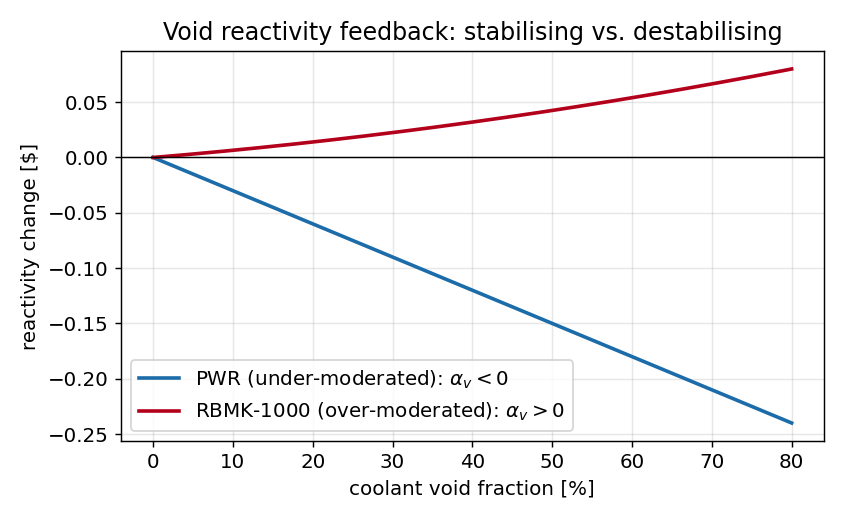
\includegraphics[width=0.74\linewidth]{figures/void.png}
\caption{The RBMK's over-moderated lattice gives a positive void coefficient
(rising curve): boiling adds reactivity, in contrast to the negative void
coefficient of an under-moderated PWR. This is the central design flaw behind
Chernobyl.}
\label{fig:void-rbmk}
\end{figure}

\section{The graphite moderator and the positive feedback chain}

The large graphite mass gave the RBMK a long prompt neutron lifetime and a great
deal of thermal inertia, which in some respects made the reactor sluggish and
seemingly forgiving. But the same graphite is what decoupled moderation from the
coolant and produced the positive void coefficient. Graphite also stores energy
(Wigner energy) and burns in air at high temperature---both relevant to the
accident's aftermath, when the exposed graphite caught fire and lofted fission
products for days. The design thus combined a destabilising neutronic
characteristic with a flammable moderator, a doubly unfortunate pairing.

\section{The fatal control-rod design}

The RBMK's most notorious flaw lay in its control rods. Each absorber rod was
fitted, on its lower end, with a \textbf{graphite ``displacer'' (follower)} about
$4.5\unit{m}$ long, separated from the boron-carbide absorber by a short column of
water. The purpose of the graphite tip was to keep water (an absorber) out of the
channel below a withdrawn rod, improving efficiency. The consequence was lethal.

When a rod was fully withdrawn, its graphite displacer sat in the central region
of the core and the lower portion of the channel was filled with water. As the rod
began to insert from the fully-withdrawn position, the leading element to enter the
core's lower region was not the boron absorber but the \emph{graphite displacer},
which \emph{displaced water} (an absorber) with \emph{graphite} (a moderator). The
immediate, local effect of beginning to insert the rod was therefore to
\emph{add} positive reactivity in the lower core---before the absorber section
arrived to add the intended negative reactivity. This is the \textbf{positive
scram effect}: pressing the emergency shutdown button could, for the first few
seconds and especially with an axially bottom-peaked flux, momentarily
\emph{increase} reactivity.

\begin{remark}[A known flaw, unaddressed]
The positive scram effect was not unknown. A similar control-rod-insertion power
spike had been observed at the Ignalina RBMK in 1983, and the phenomenon was
understood in principle. Yet the design was not corrected and operators were not
adequately warned. INSAG-7 later noted that there was a widespread belief that the
conditions under which the positive scram effect would matter ``would never
occur''---conditions that, in the event, ``appeared in almost every detail'' at
Chernobyl.
\end{remark}

\section{The operating reactivity margin}

Because the RBMK relied on a substantial number of inserted control rods to shape
its flux and maintain controllability, operating rules specified a minimum
\textbf{operating reactivity margin (ORM)}---expressed as an equivalent number of
fully-inserted control rods (nominally about $30$, with a hard floor of $15$). The
ORM was, in effect, the reactor's shutdown reserve and its guarantee of
controllability and acceptable feedback characteristics. Operating below the
minimum ORM was prohibited because it left too few absorbers to shut the reactor
down quickly and---crucially---worsened the void coefficient and the axial power
shape. On the night of the accident the ORM was driven far below the limit, to the
equivalent of perhaps six to eight rods, in the struggle against xenon poisoning.

\section{The instrumentation and protection gaps}

The RBMK's protection systems and instrumentation compounded the physical flaws.
The emergency shutdown was slow---full rod insertion took on the order of
$18\unit{s}$, an eternity for a prompt excursion. Key automatic protection
trips had been disabled to permit the test. The control system did not enforce the
ORM limit automatically. And the operators' training and documentation did not
convey the true severity of the low-power, low-ORM regime. The machine's safety
thus depended on operators avoiding a state whose danger the machine neither
prevented nor clearly signalled.

\keypoint{The RBMK-1000 combined a positive void coefficient (from graphite
moderation decoupled from water cooling), a control-rod design that added
reactivity in the first seconds of a scram (the positive scram effect), a large
core prone to spatial flux distortion, a slow shutdown system, and weak
enforcement of the operating reactivity margin. Each flaw was survivable alone; in
combination, at low power with depleted margin, they made the reactor a
prompt-excursion accident waiting for a trigger.}


\section*{Exercises}
\addcontentsline{toc}{section}{Exercises}
\begin{enumerate}[leftmargin=*,itemsep=2pt]
\item Explain how separating moderator (graphite) from coolant (water) produces a positive void coefficient.
\item Describe the positive scram effect and the role of the graphite displacers.
\item What is the operating reactivity margin, and why does operating below it worsen stability?
\item List the RBMK design features that each contributed to the accident.
\item Why was the $\sim 18\,$s shutdown time a serious weakness?
\end{enumerate}

\chapter{The Chernobyl Accident}
\label{ch:chernobyl}

On 26~April 1986, at 01:23:40 local time, an operator at Chernobyl Unit~4 pressed
the AZ-5 emergency shutdown button. Within seconds the reactor power surged to
many times its rated value, two explosions destroyed the core and building, and
the worst nuclear accident in history began. This chapter reconstructs the
sequence with the physics of the preceding chapters in hand. The aim is not to
assign blame but to show the equations playing out in a real machine.

\section{The test and its purpose}

The accident occurred during a \emph{safety test}, ironically intended to improve
the plant's response to a station blackout. The test sought to verify that, after a
loss of off-site power, the rotational inertia of a coasting-down turbine
generator could power the main coolant pumps for the brief interval before the
diesel generators reached full load. It was an electrical-engineering test of
turbine coastdown, to be run at reduced reactor power. Crucially, conducting it
required putting the reactor into a low-power state and disabling several
protective systems---taking the machine toward the corner of its operating
envelope where, as Chapter~\ref{ch:rbmk} showed, it was least stable.

\section{The descent into the unstable regime}

The test was planned for the daytime crew but was repeatedly delayed; the grid
dispatcher requested that Unit~4 keep supplying power through the evening. The
power reduction was thus stretched over many hours, during which two destabilising
processes unfolded.

\emph{Power reduction and xenon buildup.} The reactor was held at reduced power and
then, around 00:28, its thermal power fell far below the test plan---to roughly
$30\unit{MW}$ thermal, a small fraction of the $3200\unit{MW}$ rating. Accounts
differ on whether this was an operator control error or an instrumentation/control
fault; either way, the low power had a fateful consequence. During the preceding
hours at higher power the core had accumulated $^{135}$I; now, at very low flux,
xenon burnup ceased while iodine kept decaying into xenon
(Chapter~\ref{ch:xenon}). The core became heavily \textbf{xenon-poisoned}, and the
power could not easily be raised.

\emph{Rod withdrawal and loss of margin.} To fight the xenon and bring the power
back up for the test, operators withdrew control rods---many of them. By the time
power was coaxed to about $200\unit{MW}$ thermal (still well below the planned
$700\!-\!1000\unit{MW}$), the \textbf{operating reactivity margin} had fallen far
below its minimum, to the equivalent of only a handful of rods. The reactor was now
held critical by very few absorbers, with most withdrawn---the precise state in
which the void coefficient was largest, the axial flux shape distorted, and the
shutdown capability hollowed out.

\begin{figure}[H]
\centering
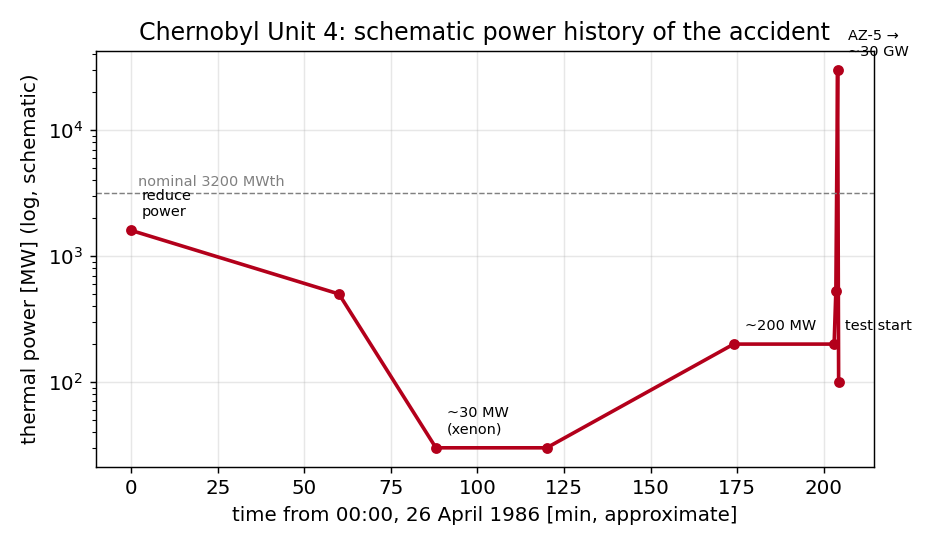
\includegraphics[width=0.92\linewidth]{figures/chernobyl_timeline.png}
\caption{Schematic thermal-power history of Chernobyl Unit~4 through the night of
the accident (illustrative, log scale). Power was reduced for the test, collapsed
to $\sim 30\unit{MW}$ with xenon poisoning, was partially recovered to
$\sim 200\unit{MW}$ by withdrawing rods, and then surged to tens of gigawatts in
seconds after AZ-5 was pressed.}
\label{fig:cher-timeline}
\end{figure}

\section{Starting the test}

With the reactor at about $200\unit{MW}$, the crew proceeded with the test rather
than aborting---a low power at which the RBMK's instability was acute. To run the
test they configured the plant in ways that further reduced safety margins:
additional main coolant pumps were running (increasing core flow, reducing
boiling and thus the steam void fraction, but pushing pumps toward cavitation),
and several automatic protection signals---including those that would have scrammed
the reactor on low water level or on the trip of the turbine---were blocked so that
the test would not be interrupted.

At 01:23:04 the turbine steam supply was closed to begin the coastdown. As the
main pumps driven by the coasting turbine slowed, core coolant flow decreased.
Less flow meant more boiling in the channels; more boiling meant more steam
\emph{voids}; and because the void coefficient was strongly positive, the voids
added reactivity. Power began to climb. In a negative-void reactor this would have
been self-correcting; in the RBMK it was self-amplifying. The reactor was now
sliding up the positive-feedback ramp.

\section{AZ-5 and the power surge}

At 01:23:40, with power rising, an operator pressed \textbf{AZ-5}, the emergency
scram, to insert all control and protection rods. What should have shut the
reactor down did the opposite---at first. As the rods began to descend from their
nearly fully-withdrawn positions, the \emph{graphite displacers} entered the lower
core first, displacing water (an absorber) and \textbf{adding} positive reactivity
in the bottom of the core (the positive scram effect of Chapter~\ref{ch:rbmk}).
Because the flux was already distorted toward the bottom of the core, this local
positive insertion struck exactly where it would do the most harm.

The added reactivity pushed the reactor through prompt criticality. Now the
physics of Chapters~\ref{ch:pk} and~\ref{ch:nonlinear} took over on the
millisecond timescale. With $\rho>\beta$, the power grew as
$\exp[(\rho-\beta)t/\Lambda]$; the positive void feedback, far from arresting the
rise, reinforced it as the surging power flashed the remaining water to steam; and
there was no sufficient prompt negative feedback to cap the excursion. The power
spiked to an estimated tens of gigawatts---perhaps a hundred times the rated
power---in a few seconds.

\section{The explosions}

The energy deposited in this prompt excursion was enormous and almost
instantaneous. The fuel overheated and fragmented; the intense heat flashed the
cooling water to steam, and the pressure surge ruptured fuel channels. The first
explosion was a \textbf{steam explosion}---the violent expansion of suddenly
generated steam---which blew off the $1000$-tonne upper biological shield
(``Elena'') and tore open the core. A second explosion followed seconds later;
its exact nature is debated (a further steam/thermal explosion, possibly with a
contribution from hydrogen generated by steam reacting with hot zirconium and
graphite, and a brief renewed criticality in the disrupted core). The explosions
demolished the reactor hall, ejected fuel and graphite, and exposed the core to
the atmosphere.

\section{The fire and the release}

With the core breached and the graphite moderator exposed to air at high
temperature, the \textbf{graphite caught fire}. The fire burned for days, lofting
fission products---$^{131}$I, $^{137}$Cs, $^{134}$Cs, and others---high into the
atmosphere, where winds carried them across the western Soviet Union and Europe.
The decay heat (Chapter~\ref{ch:decay}) in the wrecked fuel sustained high
temperatures and continued to drive releases. Emergency crews fought the fire and
later dropped boron, sand, clay, and lead from helicopters in an attempt to
smother the core and absorb neutrons. The release continued for about ten days
before subsiding.

\section{The sequence in one paragraph}

Stripped to essentials: a delayed, low-power test poisoned the core with xenon;
fighting the xenon stripped out the control rods, leaving the reactor in its most
unstable configuration with almost no shutdown margin; reducing coolant flow for
the test boiled more water, and the positive void coefficient drove power upward;
the emergency scram, through the graphite-tipped rods, added reactivity instead of
removing it and pushed the reactor prompt-critical; the positive void feedback
amplified the prompt excursion; and the resulting energy surge flashed the coolant
and exploded the core. Every step is a chapter of this book made flesh. The next
chapter analyses why, and how the understanding evolved.


\section*{Exercises}
\addcontentsline{toc}{section}{Exercises}
\begin{enumerate}[leftmargin=*,itemsep=2pt]
\item Reconstruct the chain of events from the power drop to the explosions in five steps.
\item Explain why reducing coolant flow for the test raised reactor power.
\item Why did pressing AZ-5 initially increase reactivity?
\item Estimate, qualitatively, why the excursion was over in seconds using the prompt timescale.
\item Distinguish the roles of the steam explosion and the graphite fire in the consequences.
\end{enumerate}

\chapter{Chernobyl: Root-Cause Analysis}
\label{ch:analysis}

Why did Chernobyl happen, and what did the world conclude? The answer evolved
significantly between 1986 and 1992, and the evolution is itself instructive: it is
a case study in how the apportionment of blame between ``human error'' and
``design flaw'' depends on how deeply one understands the machine. This chapter
analyses the accident through the feedback theory of Parts~II and~III and traces
the shift from INSAG-1 to INSAG-7.

\section{The accident as a feedback failure}

In the language of this book, Chernobyl was the failure of a closed-loop control
system whose loop gain became positive. Recall the stability principle: a reactor
is stable when rising temperature/power removes reactivity faster than it is added.
At Chernobyl, in its low-power, low-ORM, distorted-flux state, three feedback
elements all had the wrong sign or were too weak:

\begin{itemize}[nosep]
\item The \textbf{void coefficient} was strongly positive: rising power boiled
water, which added reactivity (Chapters~\ref{ch:feedback},~\ref{ch:rbmk}).
\item The \textbf{prompt Doppler feedback}, though negative, was too weak at low
power to overcome the void term (the fuel-temperature swings at low power are
small).
\item The \textbf{scram}, intended as the ultimate negative reactivity, was
momentarily \emph{positive} because of the graphite displacers (the positive scram
effect).
\end{itemize}

With the dominant feedbacks positive, the Nyquist locus of Chapter~\ref{ch:linear}
enclosed the critical point, and the Nordheim--Fuchs balance of
Chapter~\ref{ch:nonlinear} had no benign turnover: there was no net negative
prompt feedback to cap the excursion. The accident is, in this sense, exactly what
the stability theory predicts for a machine with these coefficients driven into
this regime. It was not an inexplicable catastrophe; it was the equations
asserting themselves.

\section{Contributing causes: a layered failure}

No single fault caused the accident; it was a chain in which each link mattered.

\textbf{Design causes.} The positive void coefficient, the positive scram effect
of the graphite-tipped rods, the slow ($\sim 18\unit{s}$) shutdown, the large core
prone to spatial flux distortion, and the lack of automatic enforcement of the
ORM---all were properties of the machine.

\textbf{Operational causes.} The test was conducted at far too low a power; the
ORM was driven far below its minimum; protective trips were disabled; and the crew
proceeded despite the reactor being in an unfamiliar and unstable state.

\textbf{Organisational and cultural causes.} The positive scram effect was known
from the 1983 Ignalina event but neither corrected nor communicated; operating
documentation understated the danger of the low-ORM regime; the test procedure was
inadequate and inadequately reviewed; and a safety culture that treated such
margins as bureaucratic rather than physical allowed the boundary to be crossed.

The deepest lesson of Chernobyl is precisely that these layers combined. A machine
with the wrong sign of feedback can be operated safely \emph{only} if the
operators rigorously avoid the regimes where that sign bites---and that requires
the organisation to know, document, and enforce those boundaries. All three failed
together.

\section{From INSAG-1 to INSAG-7: the evolution of understanding}

The International Nuclear Safety Advisory Group (INSAG) issued two major reports.

\textbf{INSAG-1 (1986)}, drawing heavily on the initial Soviet presentation,
emphasised \emph{operator error}: the violations of procedure---running at low
power, defeating protections, depleting the ORM---were presented as the primary
cause. This framing placed the weight of responsibility on the crew.

\textbf{INSAG-7 (1992)}, after the Soviet authorities released fuller information
(including the State Committee's and the Soviet scientists' own deeper analyses),
substantially revised the picture. It emphasised \emph{design deficiencies}---the
positive void coefficient and especially the positive scram effect---as root
causes, while still acknowledging the operational violations. In INSAG-7's
assessment, the operators were drawn into a trap that the reactor's physics and the
inadequate information about it had set. Its often-quoted observation is that the
conditions under which the positive scram effect would be dangerous were believed
never to occur, yet ``appeared in almost every detail'' at Chernobyl.

\begin{remark}[Why the shift matters]
The movement from ``the operators broke the rules'' to ``the machine had flaws
that made rule-breaking catastrophic, and the rules themselves were poorly
justified to those who had to follow them'' is the central interpretive lesson of
Chernobyl. It reframes safety from a matter of operator discipline alone to a
matter of \emph{inherent design}: a reactor should not be one procedure violation
away from prompt criticality, and its shutdown system should never add reactivity.
Modern safety philosophy---inherent and passive safety, defence in depth, and a
strong safety culture---descends directly from this reframing.
\end{remark}

\section{The fixes to the RBMK fleet}

After the accident the surviving RBMK reactors were extensively modified to address
the very feedback flaws this book has emphasised:
\begin{itemize}[nosep]
\item Fuel enrichment was increased (from $\sim 2\%$ toward $2.4\%$) and additional
fixed absorbers were installed, which \emph{reduced the void coefficient} so that
the power coefficient became negative across the operating range.
\item The control rods were redesigned and the displacer geometry changed to
\emph{eliminate the positive scram effect}, with faster insertion and a larger
number of rods kept inserted.
\item A hard minimum operating reactivity margin was enforced, with automatic
protection, removing the low-ORM trap.
\item Improved instrumentation and faster emergency protection were added.
\end{itemize}
These changes did not make the RBMK a Western-style reactor, but they removed the
specific positive-feedback pathways that caused the accident---an implicit
confirmation that those pathways were indeed the root cause.

\section{Comparison with Western practice}

It is worth stating plainly the contrast that makes Chernobyl so instructive.
Western light-water reactors are designed with a \emph{negative} void coefficient
and a \emph{negative} power coefficient, achieved by under-moderation; their
shutdown systems insert only negative reactivity, quickly; and their containment
buildings are designed to retain radioactivity even given core damage---a feature
the RBMK lacked. The same reactivity-insertion event that destroyed Chernobyl would
be self-limited in a PWR by its prompt negative feedback (the BORAX/SPERT result),
and any residual release would be contained. Chernobyl is thus simultaneously a
story about one flawed design and a vindication of the inherent-safety principles
embodied in others.

\keypoint{Chernobyl was a feedback failure: in its operating state the dominant
reactivity feedbacks were positive, so the coupled system was unstable and the
prompt excursion had no benign limit. The understanding evolved from blaming
operators (INSAG-1) to recognising design flaws---the positive void coefficient
and positive scram effect---as root causes (INSAG-7). The enduring lesson is that
safety must be inherent in the physics, not contingent on perfect operation.}


\section*{Exercises}
\addcontentsline{toc}{section}{Exercises}
\begin{enumerate}[leftmargin=*,itemsep=2pt]
\item Frame the accident as a feedback-loop failure using the language of Chapters 6--9.
\item Summarise the differences between INSAG-1 and INSAG-7 and why the shift matters.
\item List the design, operational, and organisational causes and argue why all three were necessary.
\item Which post-accident RBMK modifications addressed the void coefficient, and how?
\item Contrast the RBMK with a Western PWR on void coefficient, scram, and containment.
\end{enumerate}

\chapter{Decay-Heat Accidents: Three Mile Island and Fukushima}
\label{ch:decayheat-acc}

Chernobyl was a reactivity-stability accident: the fission power ran away. The two
other defining accidents of the nuclear age---Three Mile Island and
Fukushima---were the opposite kind: the reactors shut down correctly, but the
\emph{decay heat} (Chapter~\ref{ch:decay}) could not be removed. Together with
Chernobyl they complete the picture of reactor thermal safety, showing that
stopping fission is necessary but not sufficient.

\section{Three Mile Island (1979)}

At Three Mile Island Unit~2, a minor fault (a stuck-open pressuriser relief valve)
combined with misleading instrumentation led operators to throttle back the
emergency core cooling under the mistaken belief that the system was full of water.
The reactor had scrammed promptly and correctly---there was no reactivity
problem---but decay heat, initially several per cent of the $2700\unit{MW}$ thermal
rating, continued unabated. With cooling reduced, the core boiled dry in part,
overheated, and suffered substantial melting over the following hours. The
containment building, however, held, and off-site releases were minimal.

TMI's lessons were about \emph{human factors and decay heat}: control-room
instrumentation that misled rather than informed; operator training that had not
prepared the crew for the actual scenario; and the inexorability of decay heat. It
transformed operator training, control-room design, and emergency procedures
worldwide---and, seven years before Chernobyl, established that a reactor is a
thermal hazard for days after shutdown.

\section{Fukushima Daiichi (2011)}

The Fukushima Daiichi accident is the starkest demonstration of the decay-heat
imperative. A magnitude-9 earthquake caused the operating reactors to scram
correctly; fission stopped as designed. But the ensuing tsunami flooded the
emergency diesel generators and switchgear, causing a prolonged \emph{station
blackout}---a complete loss of AC power. With no power to drive cooling, decay heat
(Chapter~\ref{ch:decay}) accumulated in the cores over hours and days. The water
boiled away, the fuel overheated, the zirconium cladding reacted with steam to
generate hydrogen, and the hydrogen exploded, breaching containment in three units
and releasing radioactivity.

Fukushima was not a stability accident and not an operator-violation accident; it
was a failure to remove decay heat after a beyond-design-basis natural event
disabled the active cooling systems. Its central lesson reinforced the move toward
\emph{passive} decay-heat removal (Chapter~\ref{ch:inherent}): cooling that needs
no electrical power and no operator action for a long grace period, precisely
because the active systems can be lost.

\section{Three accidents, three lessons}

The three defining accidents form a complete syllabus of reactor thermal safety:
\begin{itemize}[nosep]
\item \textbf{Chernobyl (1986)}---a \emph{reactivity-stability} failure: positive
feedback and a flawed scram drove a prompt-critical excursion. Lesson: inherent
negative feedback and a sound shutdown system are non-negotiable.
\item \textbf{Three Mile Island (1979)}---a \emph{decay-heat plus human-factors}
failure: correct scram, but cooling was throttled and the core melted. Lesson:
instrumentation, training, and respect for decay heat.
\item \textbf{Fukushima (2011)}---a \emph{decay-heat plus station-blackout}
failure: correct scram, but a natural disaster disabled active cooling. Lesson:
passive, power-independent decay-heat removal.
\end{itemize}
Stability (the subject of this book) addresses the first; passive decay-heat
removal addresses the second and third. A reactor that is both inherently stable
\emph{and} passively cooled is safe against all three failure modes---the goal of
modern design.

\keypoint{Not every reactor accident is a stability accident. TMI and Fukushima
shut down correctly but could not remove decay heat---one through human factors,
one through a natural disaster that disabled active cooling. Thermal safety
therefore demands both inherent stability (against excursions) and passive
decay-heat removal (against loss of cooling).}

\section*{Exercises}
\addcontentsline{toc}{section}{Exercises}
\begin{enumerate}[leftmargin=*,itemsep=2pt]
\item Classify TMI, Fukushima, and Chernobyl by failure mode (reactivity vs.\ decay heat).
\item Explain why correct scram did not prevent core damage at TMI and Fukushima.
\item What is a station blackout, and why is it central to Fukushima?
\item Argue why passive decay-heat removal addresses the Fukushima failure mode.
\item State the single lesson each of the three accidents contributes to thermal safety.
\end{enumerate}


\part{Modern Practice and Synthesis}
\chapter{Inherent and Passive Safety in Modern Designs}
\label{ch:inherent}

The lesson of Chernobyl---that safety must live in the physics, not in perfect
operation---has shaped reactor design ever since. This chapter surveys how modern
reactors build in negative feedback and passive heat removal so that thermal
stability and decay-heat safety are guaranteed by nature rather than by
intervention.

\section{Inherent vs.\ engineered safety}

\emph{Engineered} safety relies on active systems---pumps, valves, diesel
generators, operator actions---to respond to upsets. \emph{Inherent} safety relies
on the physical properties of the reactor: feedback coefficients, material
choices, and geometry that make dangerous states physically self-correcting or
unreachable. \emph{Passive} safety relies on natural forces---gravity, natural
circulation, conduction, stored coolant---that need no power or operator action.
The modern ideal combines all three with defence in depth, but assigns the
foundational role to inherent and passive features, precisely because Chernobyl,
TMI, and Fukushima showed that active systems and operators can fail.

\section{Designing in negative feedback}

The first principle is a \textbf{negative power coefficient across all operating
states}. This is achieved through:
\begin{itemize}[nosep]
\item \textbf{Under-moderation} in light-water reactors, guaranteeing negative
moderator and void coefficients (the opposite of the RBMK).
\item Strong \textbf{Doppler feedback} from fertile resonance absorbers
($^{238}$U, $^{240}$Pu), giving a prompt negative coefficient that limits
excursions.
\item Avoidance of positive void pathways: no graphite-decoupled-from-coolant
geometry, and shutdown systems that insert only negative reactivity.
\end{itemize}
Licensing in most countries requires demonstrating a negative power coefficient and
analysing reactivity-initiated accidents to show self-limitation. The RBMK's
positive void coefficient would not be licensable under such rules.

\section{Passive decay-heat removal}

Because decay heat (Chapter~\ref{ch:decay}) is irreducible, modern designs provide
\emph{passive} paths to remove it without power. Examples include gravity-driven
core flooding, natural-circulation cooling loops, large elevated water pools that
boil off over days, and---in some advanced designs---heat conduction to the ground
or air. The goal is a reactor that can survive a complete station blackout (as at
Fukushima) for an extended ``grace period'' with no operator action and no
electrical power. The AP1000, for instance, is designed to remove decay heat
passively for about three days using stored water and natural circulation.

\section{Generation III+ light-water reactors}

Evolutionary designs (AP1000, EPR, and others) retain the proven negative-feedback
physics of the PWR and add passive safety systems, larger water inventories,
core-catchers to contain molten fuel, and digital protection. They are, in
stability terms, conservative: their inherent feedback is strongly negative and
their innovations are mostly in passive heat removal and containment. They embody
the direct engineering response to the failure modes of TMI, Chernobyl, and
Fukushima.

\section{Generation IV and advanced reactors}

More radical designs pursue inherent safety through different physics:
\begin{itemize}[nosep]
\item \textbf{High-temperature gas reactors} (HTGR) use TRISO fuel particles that
retain fission products to very high temperatures and a core whose large negative
temperature coefficient and low power density allow it to shed decay heat by
conduction and radiation alone---it cannot melt even with no cooling.
\item \textbf{Molten-salt reactors} carry fuel dissolved in a liquid salt with a
strongly negative temperature/expansion coefficient and a passive
``freeze-plug'' drain that empties the core into safe geometry on loss of power.
\item \textbf{Sodium-cooled fast reactors} can be designed with strong negative
expansion feedback; the EBR-II tests in 1986---the same year as Chernobyl---famously
demonstrated survival of a complete loss of flow \emph{without scram} purely
through inherent feedback.
\item \textbf{Lead-cooled and heat-pipe microreactors} pursue similar
walk-away-safe goals with passive heat transport.
\end{itemize}
The unifying theme is the same principle this book has developed: make the
dominant feedback strongly negative and provide a passive path for decay heat, so
that the reactor is safe \emph{by physics}.

\section{The EBR-II demonstration: the anti-Chernobyl}

It is worth pausing on a remarkable coincidence of timing. On 3~April 1986---just
three weeks before Chernobyl---engineers at the Experimental Breeder Reactor~II
(EBR-II) in Idaho deliberately subjected the reactor to a complete
\emph{loss-of-flow-without-scram} test at full power: they cut the coolant pumps
and disabled the automatic shutdown. Rather than melting, the reactor's strong
\emph{negative} reactivity feedback (from thermal expansion of the metallic fuel
and structure) reduced the power as temperatures rose, and the reactor settled to a
safe, low-power state on its own. The same week, two reactors on opposite sides of
the world were pushed beyond their protection systems; one destroyed itself and a
region, the other quietly proved that inherent negative feedback is the surest
safety system of all. The contrast is the thesis of this book in a single image.

\keypoint{Modern reactor safety is founded on inherent negative feedback (a
negative power coefficient guaranteed across all states) and passive decay-heat
removal (natural forces that need no power or operators). EBR-II's 1986
loss-of-flow-without-scram test is the positive mirror image of Chernobyl:
inherent negative feedback turning a would-be accident into a non-event.}



\section{The quasi-static reactivity balance and integral safety parameters}
\label{sec:qsrb}

The qualitative claim that inherent feedback ``shuts the reactor down'' can be made
quantitative through the \emph{quasi-static reactivity balance} (QSRB) of Wade and
Fujita, the analytical backbone of metal-fuelled fast-reactor passive safety. For
transients slow compared with the prompt and delayed-neutron timescales, the
reactor passes through a sequence of near-critical states in which the net
reactivity is approximately zero. Writing $\tilde P=P/P_0$ for normalised power and
$\tilde F=F/F_0$ for normalised flow, the asymptotic balance reads
\begin{equation}
0=\delta\rho_{\rm ext}+(\tilde P-1)\,A+\Big(\tfrac{\tilde P}{\tilde F}-1\Big)B
   +\delta T_{\rm in}\,C,
\label{eq:qsrb}
\end{equation}
where the \emph{integral reactivity parameters} are
\begin{equation}
A=P_0\frac{\partial\rho}{\partial P}\ (\text{power coefficient}\times P_0),\quad
B=\text{power/flow coefficient},\quad
C=\frac{\partial\rho}{\partial T_{\rm in}}\ (\text{inlet-temperature coefficient}),
\end{equation}
with $A<0$ (Doppler $+$ axial fuel expansion) and $B<0$ (coolant-density/radial
expansion) for an inherently safe core. Equation \eqref{eq:qsrb} compresses all the
feedbacks of Chapter~\ref{ch:feedback} into three measurable integral numbers.

\begin{proposition}[Asymptotic power of an unprotected loss of flow]
\label{prop:ulof}
For an unprotected loss-of-flow transient (ULOF: $\delta\rho_{\rm ext}=0$,
$\delta T_{\rm in}=0$, flow decaying to $\tilde F<1$) the asymptotic power is
\begin{equation}
\tilde P_\infty=\frac{A+B}{A+B/\tilde F},
\end{equation}
which satisfies $0<\tilde P_\infty<1$ whenever $A,B<0$; the core settles to a
reduced power without scram. The asymptotic coolant temperature rise across the
core obeys $\Delta T_c^\infty/\Delta T_c^0=\tilde P_\infty/\tilde F$.
\end{proposition}
\begin{proof}
Set $\delta\rho_{\rm ext}=\delta T_{\rm in}=0$ in \eqref{eq:qsrb}:
$(\tilde P-1)A+(\tilde P/\tilde F-1)B=0$, i.e.\ $\tilde P(A+B/\tilde F)=A+B$, giving
$\tilde P_\infty$. With $A,B<0$ and $0<\tilde F<1$, both numerator and denominator
are negative and the denominator is larger in magnitude, so
$0<\tilde P_\infty<1$. The temperature ratio follows from
$\Delta T_c\propto P/F$.
\end{proof}

The dimensionless ratios $A/B$ and $C\,\Delta T_c/A$ are the modern \emph{passive
safety metrics}: a design with $A/B\approx1$ and small $|C\,\Delta T_c/A|$ rides
out the unprotected ULOF, ULOHS (loss of heat sink), and UTOP (transient
overpower) accidents with asymptotic temperatures below failure limits---the
analytic statement of the EBR-II demonstrations.

\section{Passive decay-heat removal: natural-circulation scaling}
\label{sec:natcirc}

Passive cooling replaces pumps with buoyancy. In a closed loop of thermal-centre
elevation difference $\Delta z$, the buoyancy head balances friction:
\begin{equation}
\underbrace{\rho_0\,\beta_{\rm th}\,g\,\Delta z\,\Delta T_{\rm loop}}_{\text{buoyancy}}
=\underbrace{R_f\,\dot m^2}_{\text{friction}},\qquad
R_f=\frac{1}{2\rho_0 A_{\rm fl}^2}\Big(\frac{fL}{D}+\textstyle\sum K\Big),
\end{equation}
with $\beta_{\rm th}$ the thermal expansion coefficient and
$\Delta T_{\rm loop}=Q/(\dot m c_p)$ the loop temperature rise carrying power $Q$.

\begin{proposition}[One-third power law]
\label{prop:natcirc}
Eliminating $\Delta T_{\rm loop}$ gives the natural-circulation mass flow and
temperature rise
\begin{equation}
\dot m=\Big(\frac{\rho_0\beta_{\rm th}g\Delta z}{c_p R_f}\Big)^{1/3}Q^{1/3},
\qquad
\Delta T_{\rm loop}=\frac{Q}{c_p\dot m}\propto Q^{2/3}.
\end{equation}
Hence the coolant temperature rise grows only as $Q^{2/3}$: as decay heat falls
after shutdown, natural circulation self-adjusts and the temperature rise decays
sublinearly, the quantitative basis of multi-day passive grace periods.
\end{proposition}
\begin{proof}
Substitute $\Delta T_{\rm loop}=Q/(\dot m c_p)$ into the head--friction balance:
$\rho_0\beta_{\rm th}g\Delta z\,Q/(\dot m c_p)=R_f\dot m^2$, so
$\dot m^3=\rho_0\beta_{\rm th}g\Delta z\,Q/(c_p R_f)$, giving the stated
$\dot m\propto Q^{1/3}$ and therefore $\Delta T_{\rm loop}=Q/(c_p\dot m)\propto
Q/Q^{1/3}=Q^{2/3}$.
\end{proof}

\section{Conduction-cooled cores and the radiative walk-away criterion}
\label{sec:walkaway}

In a high-temperature gas or microreactor core with no active cooling, decay heat
leaves by conduction to the vessel and thence by radiation to a passive heat sink.
Modelling the vessel as a grey radiator of area $A_s$ and emissivity
$\varepsilon$, energy balance at the quasi-steady decay power $P_d$ gives
\begin{equation}
\varepsilon\sigma A_s\big(T_{\rm eq}^4-T_{\rm amb}^4\big)=P_d
\ \Longrightarrow\
T_{\rm eq}=\Big(\frac{P_d}{\varepsilon\sigma A_s}+T_{\rm amb}^4\Big)^{1/4}.
\label{eq:radeq}
\end{equation}
Adding the internal conduction rise from a distributed source $q'''$ across a core
of conductivity $k$ and characteristic radius $R$ (cylindrical, parabolic profile)
$\Delta T_{\rm cond}=q''' R^2/(4k)=P_d/(8\pi k H)$ for height $H$, the peak fuel
temperature is $T_{\max}=T_{\rm eq}+\Delta T_{\rm cond}$.

\begin{definition}[Walk-away-safe core]
A core is \emph{walk-away safe} against a complete, unmitigated loss of cooling if
its peak passive temperature satisfies $T_{\max}<T_{\rm fail}$, where
$T_{\rm fail}$ is the fuel-failure temperature (e.g.\ $\sim1600\degC$ for TRISO
fuel). By \eqref{eq:radeq} this requires the power density to be low enough that
$T_{\rm eq}+P_d/(8\pi k H)<T_{\rm fail}$, a constraint that scales favourably as
core size shrinks ($A_s/V$ rises), explaining the passive safety of small modular
and micro-reactors.
\end{definition}

Because $T_{\rm eq}\propto P_d^{1/4}$ while the failure margin is fixed, the
walk-away criterion is fundamentally a \emph{power-density} limit: it caps the
admissible $P_d/A_s$, and through the decay-heat fraction (Chapter~\ref{ch:decay}),
the admissible operating power density---a recurring constraint in Generation-IV
design optimisation~\cite{waltar}.


\section*{Exercises}
\addcontentsline{toc}{section}{Exercises}
\begin{enumerate}[leftmargin=*,itemsep=2pt]
\item Distinguish inherent, passive, and engineered safety with an example of each.
\item Explain how under-moderation guarantees a negative void coefficient.
\item Describe one passive decay-heat removal strategy and the grace period it provides.
\item Summarise the EBR-II 1986 loss-of-flow-without-scram test and why it is the ``anti-Chernobyl''.
\item For an HTGR with TRISO fuel, explain why the core ``cannot melt'' even without active cooling.
\end{enumerate}

\chapter{Computational Modelling of Reactor Dynamics}
\label{ch:comp}

The theory of the preceding chapters becomes vivid when integrated numerically.
This chapter describes a small, open-source point-reactor-kinetics toolkit written
to accompany this book, shows the transients it produces, and uses it to make the
stability principles concrete---including a numerical caricature of the Chernobyl
feedback failure.

\section{A minimal point-kinetics solver}

The companion code, \texttt{reactor-kinetics}, couples validated delayed-neutron
data to a stiff ODE integrator with optional temperature feedback. Its core is the
six-group point kinetics of Chapter~\ref{ch:pk} together with the adiabatic
feedback model of Chapters~\ref{ch:thermal} and~\ref{ch:nonlinear}:
\begin{align*}
\frac{\dd p}{\dd t} &= \frac{\rho(t)-\beta}{\Lambda}p + \sum_i\lambda_i\zeta_i,\quad
\frac{\dd \zeta_i}{\dd t} = \frac{\beta_i}{\Lambda}p - \lambda_i\zeta_i,\\
\frac{\dd T}{\dd t} &= \frac{P_0\,p}{C},\qquad
\rho(t) = \rho_{ext}(t) + \alpha\,(T-T_0).
\end{align*}
Because $\Lambda\sim 10^{-5}\unit{s}$ while the precursor times are seconds, the
system is stiff; the solver uses an implicit/adaptive method (LSODA). Delayed-neutron
parameters are taken from validated $^{235}$U data (Appendix~\ref{app:data}).

\section{Verification against the inhour equation}

A dynamics code is only trustworthy if it reproduces known analytical results. The
toolkit's asymptotic period, measured from simulated power traces, matches the
inhour equation \eqref{eq:inhour} to better than $10^{-4}$ across a range of step
reactivities (Figure~\ref{fig:inhour}). This agreement validates both the solver
and the kinetics implementation, and it reproduces the steep collapse of the period
as reactivity approaches one dollar---the quantitative warning sign of approaching
prompt criticality.

\section{A gallery of transients}

Figure~\ref{fig:transients} collects four canonical transients computed with the
toolkit, each illustrating a principle from earlier chapters:

\begin{enumerate}[nosep]
\item \textbf{Sub-prompt step ($+0.3\$$).} A prompt jump
(Eq.~\ref{eq:promptjump}) followed by a slow rise on a stable delayed-neutron
period---the controllable regime.
\item \textbf{Prompt-critical step ($+1.2\$$).} Runaway growth on the prompt
timescale (note the logarithmic axis), the signature of crossing one dollar.
\item \textbf{Control-rod scram.} A negative ramp drives the power down, with the
characteristic delayed-neutron tail as the precursors decay.
\item \textbf{Reactivity-initiated excursion with feedback.} A prompt-critical
insertion limited by negative temperature feedback: the power peaks and turns
over, the Nordheim--Fuchs self-limitation of Chapter~\ref{ch:nonlinear}.
\end{enumerate}

The fourth panel is the crux. With negative feedback the excursion is capped and
the reactor survives. The exercise below shows what happens when the feedback sign
is wrong.

\section{A numerical caricature of the Chernobyl feedback failure}

The toolkit makes it easy to flip the sign of the feedback and watch stability
turn into instability. Consider two runs with identical prompt-critical insertions
($\rho_0\approx 1.05\$$):

\begin{itemize}[nosep]
\item \textbf{Negative feedback} ($\alpha<0$, the well-designed reactor): the
fuel heats, reactivity falls, and the power excursion turns over at a finite peak,
depositing a bounded energy $E_{\text{total}}\approx 2(\rho_0-\beta)/\gamma$
(Chapter~\ref{ch:nonlinear}). The reactor self-limits.
\item \textbf{Positive feedback} ($\alpha>0$, the Chernobyl-like configuration):
the rising power adds further reactivity, there is no turnover, and the power grows
until the model's adiabatic assumptions break---representing, in reality, fuel
fragmentation, coolant flashing, and disassembly.
\end{itemize}

This two-line change in a parameter reproduces, in caricature, the essential
physics of the accident: the difference between Chernobyl and a survivable RIA is
the \emph{sign of} $\alpha$. The toolkit also includes a model void/temperature
feedback that becomes positive at low ``power,'' qualitatively mimicking the RBMK's
low-power instability window of Chapter~\ref{ch:linear}.

\begin{remark}[On responsible modelling]
The companion code is an educational point-kinetics tool. It is deliberately
\emph{not} a high-fidelity simulation of any specific reactor: it uses lumped
parameters, an adiabatic feedback, and generic data. Its value is pedagogical---to
let a reader reproduce the inhour equation, watch a prompt-critical excursion, and
see negative feedback cap it---not to model a real plant, which requires validated,
qualified codes (e.g.\ coupled neutronics/thermal-hydraulics systems) far beyond a
point model.
\end{remark}

\section{Toward higher fidelity}

Real safety analysis goes well beyond point kinetics. Spatial effects
(Chapter~\ref{ch:xenon}) demand at least nodal or full three-dimensional
neutronics coupled to a multi-channel thermal-hydraulics solver; the RBMK's size
made such spatial modelling essential, and core-average point parameters
understated the danger. Modern coupled codes solve the time-dependent
neutron-transport (or diffusion) equation on a spatial mesh, feed local powers to a
thermal-hydraulic subchannel model, and return local temperatures and densities as
feedback---closing the loop of Chapter~\ref{ch:coupled} cell by cell. The point
model of this chapter is the conceptual seed of those codes, and the place to build
intuition before trusting their output.

\keypoint{A small point-kinetics code reproduces the inhour equation to $10^{-4}$,
displays the canonical transients, and---by flipping the sign of the feedback
coefficient---turns a self-limiting excursion into a Chernobyl-like runaway. The
sign of the feedback is, numerically as well as physically, the whole story.}



\section{Stiffness and absolute stability}
\label{sec:stiffness}

The point-kinetics generator $\mathbf M$ has eigenvalues spanning
$|s_0|\sim\lambda_i\sim10^{-2}$--$10^{0}\unit{s^{-1}}$ up to
$|s_G|\sim\beta/\Lambda\sim10^{3}\unit{s^{-1}}$, a \emph{stiffness ratio}
\begin{equation}
S=\frac{\max_j|\Re s_j|}{\min_j|\Re s_j|}\sim\frac{\beta/\Lambda}{\lambda_1}
\sim10^{5}\text{--}10^{6}.
\end{equation}
An explicit method applied to a mode $\dot y=s y$ is stable only if $hs$ lies in
its bounded region of absolute stability; for forward Euler this requires
$h<2/|s_G|\sim2\Lambda\sim10^{-5}\unit{s}$, prohibitively small. Implicit methods
remove this restriction.

\begin{definition}[A- and L-stability]
A one-step method with stability function $R(z)$ (the amplification for
$\dot y=sy$, $z=hs$) is \emph{A-stable} if its stability region contains the entire
left half-plane, $|R(z)|\le1$ for all $\Re z\le0$. It is \emph{L-stable} if in
addition $R(z)\to0$ as $\Re z\to-\infty$ (rapid damping of the stiffest modes).
\end{definition}

\begin{theorem}[$\theta$-method stability]
\label{thm:theta}
The $\theta$-method $y_{n+1}=y_n+h[(1-\theta)f_n+\theta f_{n+1}]$ has
$R(z)=\dfrac{1+(1-\theta)z}{1-\theta z}$. It is A-stable iff $\theta\ge\tfrac12$;
the trapezoidal rule $\theta=\tfrac12$ is A-stable but not L-stable
($R(-\infty)=-1$), while backward Euler $\theta=1$ is L-stable
($R(-\infty)=0$).
\end{theorem}
\begin{proof}
Apply the method to $\dot y=sy$: $y_{n+1}=R(z)y_n$ with the stated $R$. For
$\Re z\le0$, $|R(z)|\le1\iff|1+(1-\theta)z|\le|1-\theta z|$; squaring and
simplifying gives $(1-2\theta)|z|^2\le -2\Re z\,(\,\cdot\,)$ which holds for all
$\Re z\le0$ iff $1-2\theta\le0$, i.e.\ $\theta\ge\tfrac12$. The limits
$R(-\infty)=(\theta-1)/\theta$ give $-1$ at $\theta=\tfrac12$ and $0$ at
$\theta=1$.
\end{proof}

The backward-differentiation formulas (BDF$k$) used by production solvers (e.g.\
LSODA, CVODE) are $A(\alpha)$-stable up to order $6$ and L-stable at orders $1$--$2$;
their use is what makes the figures of this book reproducible at large step sizes.

\section{Exponential and operator-splitting integrators}
\label{sec:expint}

Because the point-kinetics block is \emph{linear} in $\mathbf y$ for fixed $\rho$,
the exact one-step propagator over an interval of constant reactivity is the matrix
exponential
\begin{equation}
\mathbf y_{n+1}=e^{\mathbf M(\rho_n)\,h}\,\mathbf y_n,
\label{eq:expprop}
\end{equation}
which is unconditionally stable and exact for piecewise-constant $\rho$ (the
``analytic-within-a-step'' / PCA method). For time-varying $\rho$ the
piecewise-constant approximation incurs a local error $\mathcal O(h^2\dot\rho)$.
The action $e^{\mathbf M h}\mathbf v$ need not be formed densely; Krylov-subspace
methods compute it in $\mathcal O(m)$ matvecs via
$e^{\mathbf M h}\mathbf v\approx\|\mathbf v\|\,V_m e^{H_m h}e_1$, where $(V_m,H_m)$
is the Arnoldi factorisation of $\mathbf M$~\cite{molervanloan}.

For the \emph{coupled} neutronic--thermal system, Strang operator splitting advances
the neutronic flow $\Phi^N$ and thermal flow $\Phi^T$ as
\begin{equation}
\mathbf y_{n+1}=\Phi^N_{h/2}\circ\Phi^T_{h}\circ\Phi^N_{h/2}\,\mathbf y_n,
\end{equation}
with global error $\mathcal O(h^2)$ provided each sub-flow is solved at least to
second order; the splitting error is governed by the commutator $[\mathbf
M_N,\mathbf M_T]$ and vanishes when the blocks commute.

\section{Error bounds via the logarithmic norm}
\label{sec:lognorm}

Classical Lipschitz error bounds are useless for stiff systems (the Lipschitz
constant is $\sim|s_G|$). The sharp tool is the \emph{logarithmic norm}
$\mu(\mathbf M)=\lim_{h\to0^+}(\|\mathbf I+h\mathbf M\|-1)/h$; in the $2$-norm
$\mu_2(\mathbf M)=\lambda_{\max}\!\big(\tfrac12(\mathbf M+\mathbf M^{\!\top})\big)$.

\begin{theorem}[One-sided error bound]
\label{thm:lognorm}
If the exact and numerical flows satisfy $\dot{\mathbf x}=\mathbf M\mathbf x$ with
local truncation error $\boldsymbol\tau_n$, the global error
$\mathbf e_n=\mathbf x_n-\mathbf x(t_n)$ obeys
\begin{equation}
\|\mathbf e_n\|\le e^{\mu(\mathbf M)\,t_n}\|\mathbf e_0\|
+\sum_{k=1}^{n}e^{\mu(\mathbf M)(t_n-t_k)}\|\boldsymbol\tau_k\|.
\end{equation}
\end{theorem}
\begin{proof}[Sketch]
From $\dot{\mathbf e}=\mathbf M\mathbf e+\boldsymbol\tau$, the differential
inequality $\dfrac{\dd}{\dd t}\|\mathbf e\|\le\mu(\mathbf M)\|\mathbf
e\|+\|\boldsymbol\tau\|$ holds because
$\dfrac{\dd}{\dd t}\|\mathbf e\|\le\mu(\mathbf M)\|\mathbf e\|$ for the homogeneous
part; Gr\"onwall's inequality then yields the bound.
\end{proof}

The bound is informative precisely when $\mu(\mathbf M)$ is small or negative
(stable, damped dynamics) even though $\|\mathbf M\|$ is enormous; for a
prompt-critical excursion $\mu(\mathbf M)>0$ and the bound correctly predicts
exponential error growth---a quantitative warning that fast excursions demand
tight tolerances. This B-convergence framework~\cite{hairerwanner} is the modern
foundation for trusting stiff reactor-kinetics solvers.


\section*{Exercises}
\addcontentsline{toc}{section}{Exercises}
\begin{enumerate}[leftmargin=*,itemsep=2pt]
\item Why must a point-kinetics solver use a stiff integration method?
\item Describe how to validate a dynamics code against the inhour equation.
\item Explain what changes in the model output when the feedback coefficient sign is flipped.
\item What are the limitations of a lumped point-kinetics model for analysing a real, large reactor?
\item Outline what a higher-fidelity coupled neutronics/thermal-hydraulics code adds over a point model.
\end{enumerate}

\chapter{Synthesis and Conclusions}
\label{ch:synth}

We have travelled from the neutron balance to the ruins of Chernobyl Unit~4. This
closing chapter draws the threads together into a small number of durable
principles.

\section{The one-sentence theory}

If this book could be compressed to a sentence, it is this:
\begin{quote}
\emph{A reactor is thermally stable if and only if a rise in power removes
reactivity---through temperature and density feedback---faster and more surely than
the rise in power can add it; and this must hold promptly, and at every power
level and core state the reactor can reach.}
\end{quote}
Every chapter is an elaboration. Point kinetics
(Chapter~\ref{ch:pk}) sets the timescale on which ``faster'' must be measured and
identifies one dollar as the cliff edge. Thermal transport
(Chapter~\ref{ch:thermal}) sets how quickly temperature follows power, and which
feedbacks are prompt. The feedback coefficients (Chapter~\ref{ch:feedback}) supply
the signs and magnitudes. Stability theory (Part~III) turns ``faster and more
surely'' into eigenvalues and Nyquist loci. And Chernobyl (Part~IV) shows what the
violation looks like.

\section{Five principles of thermally stable design}

\textbf{1.\ A negative power coefficient, always.} The aggregate of all
temperature/void feedbacks must remove reactivity as power rises, at every
operating point. This single property makes a reactor self-regulating. The RBMK's
low-power positive coefficient was the root flaw.

\textbf{2.\ Prompt negative feedback to cap excursions.} Doppler feedback, being
prompt and reliably negative, is the only defence against a prompt-critical
excursion. A reactor must have enough of it that the net prompt feedback is
negative even with the void term included.

\textbf{3.\ A shutdown system that only ever helps.} The emergency shutdown must
insert negative reactivity, quickly, under all conditions. A scram that can add
reactivity---as the RBMK's graphite-tipped rods did---is a contradiction in terms
and was decisive at Chernobyl.

\textbf{4.\ Respect the slow instabilities and the memory.} Xenon poisoning and
spatial oscillations give the reactor an hours-long memory and can make a large
core locally unstable even when globally benign. Operation must account for
history and spatial shape, and negative feedback must be strong enough to damp
spatial modes.

\textbf{5.\ Plan for the heat that will not switch off.} Decay heat is several per
cent of full power for a long time after shutdown. A passive, reliable path to the
ultimate heat sink must always exist---the lesson of TMI and Fukushima as much as
of Chernobyl.

\section{The human and organisational dimension}

The physics is necessary but not sufficient. Chernobyl's deepest lesson, captured
in the shift from INSAG-1 to INSAG-7, is that a machine with marginal or wrong-sign
feedback places an impossible burden on its operators: it asks them never to enter
states whose danger they were never properly told about. Safety culture---honest
documentation, conservative procedures, the freedom to halt a test, and the
humility to treat margins as physics rather than paperwork---is itself a part of
the safety system. The best reactors reduce this burden by being inherently safe;
the best organisations carry what remains of it conscientiously.

\section{The two reactors of April 1986}

We end where the contrast is sharpest. In April~1986, two reactors were
deliberately pushed past their protection systems. At EBR-II in Idaho, engineers
cut the coolant flow at full power without scram, and the reactor's strong negative
feedback quietly brought it to a safe state---a planned demonstration of inherent
safety. Three weeks later at Chernobyl, a reactor with a positive void coefficient
and a flawed scram was driven into its least stable regime, and its physics tore it
apart. Same era, same act of pushing a reactor past its protections, opposite
outcomes---decided by the \emph{sign of the feedback}. That sign is the whole of
thermal stability, and it is the legacy that the victims of Chernobyl bequeathed to
every reactor designed since.

\section{Closing}

Thermal stability is not an exotic corner of reactor physics; it is the property
that makes nuclear power possible. Understood, it yields machines that ride out
disturbances and shut themselves down. Ignored or got wrong, it yields Chernobyl.
The mathematics in this book is, in the end, a long and careful way of saying
something simple: build reactors whose own nature opposes their excursions, and
never operate a reactor in a state where that nature is reversed.



\section{A dimensionless formulation and the master stability inequality}
\label{sec:dimensionless}

The recurring results of this book collapse into a single dimensionless statement.
Nondimensionalise the one-temperature feedback model (\S\ref{sec:statespace}) with
$\hat t=\lambda t$, normalised power $p=P/P_0$, and scaled temperature
$\vartheta=(T-T_0)/\Delta T_{\rm ref}$, $\Delta T_{\rm ref}=P_0/(\mu\lambda)$.
Three dimensionless groups emerge:
\begin{equation}
\epsilon=\frac{\Lambda\lambda}{\beta}\ (\text{prompt-to-delayed ratio}),\quad
\mathcal D=\frac{|\alpha|\,P_0}{\mu\lambda\,\beta}\ (\text{Doppler/feedback number}),\quad
\Theta=\frac{\theta}{\lambda}\ (\text{cooling-to-decay ratio}),
\end{equation}
where $\epsilon\sim10^{-3}$ is tiny (delayed neutrons dominate),
$\mathcal D$ measures feedback strength in dollars per reference temperature, and
$\Theta$ compares heat removal to precursor decay.

\begin{theorem}[Master stability inequality]
\label{thm:master}
In the dimensionless variables the critical-equilibrium Jacobian has characteristic
polynomial $\hat s^3+\hat a_1\hat s^2+\hat a_2\hat s+\hat a_3$ with
$\hat a_3=\operatorname{sign}(\alpha)\,\mathcal D\,\Theta$. The operating point is
asymptotically stable if and only if
\begin{equation}
\boxed{\ \alpha<0\quad\text{and}\quad \mathcal D>0,\ \Theta>0\ }
\end{equation}
i.e.\ the feedback is negative and both the feedback and cooling are nonzero;
equivalently $\hat a_3>0$ together with the Routh--Hurwitz product
$\hat a_1\hat a_2>\hat a_3$, which holds automatically when $\alpha<0$. The single
controlling parameter is therefore the \emph{sign of} $\mathcal D$ inherited from
$\alpha$.
\end{theorem}
\begin{proof}
Nondimensionalising $\mathbf A$ of \S\ref{sec:statespace} rescales each coefficient
of the characteristic polynomial by positive factors, preserving the signs;
$\hat a_3\propto-\alpha$ as in \eqref{eq:rh-coeffs}. Proposition~\ref{prop:stab}
then applies verbatim: stability $\iff\alpha<0$.
\end{proof}

Theorem~\ref{thm:master} is the book in one line: across six orders of magnitude in
timescale and every chapter of physics, linear stability of the operating point is
controlled by the sign of a single dimensionless feedback number. The Chernobyl
state had $\mathcal D<0$ (effective $\alpha>0$ from the positive void coefficient),
placing it on the unstable side of the boxed inequality.

\section{Open problems and directions}
\label{sec:open}

The reduced models of this book invite several graduate-level extensions, each an
active research direction:
\begin{itemize}[leftmargin=*]
\item \textbf{Spatial kinetics.} Replacing point kinetics with the time-dependent
multigroup transport (or $SP_3$/diffusion) equations coupled to subchannel
thermal-hydraulics; the relevant stability object is the spectrum of an
infinite-dimensional operator, and modal (lambda-mode) reduction connects it to the
finite analysis here.
\item \textbf{Circulating-fuel reactors.} In molten-salt reactors the precursors
drift with the fuel, modifying \eqref{eq:prk} to a delay/advection system
$\dot C_i=\beta_i p/\Lambda-\lambda_iC_i-C_i/\tau_{\rm loop}+C_i(t-\tau_{\rm loop})e^{-\lambda_i\tau_{\rm loop}}$,
whose effective $\beta$ is reduced---a genuinely different stability problem.
\item \textbf{Stochastic kinetics.} At low power the discrete neutron number makes
the master equation, not the ODE, fundamental; the stability of moments and the
$\alpha$-Feynman / Rossi variance methods quantify fluctuations.
\item \textbf{Robust and nonlinear control.} Treating $\alpha$, $\Lambda$, and the
thermal parameters as uncertain leads to $\mu$-synthesis and Lyapunov-based bounds
on the guaranteed stability margin over the operating envelope.
\end{itemize}
These carry the linear, lumped theory of this book toward the high-fidelity,
uncertainty-aware models used in contemporary reactor-safety research.


\section*{Exercises}
\addcontentsline{toc}{section}{Exercises}
\begin{enumerate}[leftmargin=*,itemsep=2pt]
\item State the one-sentence theory of thermal stability in your own words.
\item List the five principles of thermally stable design and give the Chernobyl counter-example for each.
\item Argue why safety culture is part of the safety system, citing the INSAG-1 to INSAG-7 shift.
\item Compare the EBR-II and Chernobyl events of April 1986 and state what single quantity decided their outcomes.
\item In what sense is thermal stability ``the property that makes nuclear power possible''?
\end{enumerate}


% ===========================================================================
%  APPENDICES
% ===========================================================================
\appendix
\part*{Appendices}
\addcontentsline{toc}{part}{Appendices}
\chapter{Delayed-Neutron and Kinetics Data}
\label{app:data}

The transients and figures in this book use the six-group delayed-neutron data for
thermal fission of $^{235}$U listed in Table~\ref{tab:delayed}. These values are
representative of the validated parameters distributed with the PyRK package and
are consistent with standard compilations (Keepin; ENDF-derived sets). The total
delayed fraction is $\beta=\sum_i\beta_i$, and a representative prompt neutron
generation time for a thermal system is $\Lambda\approx 1.1\times10^{-5}\unit{s}$.

\begin{table}[H]
\centering
\caption{Six-group delayed-neutron data for thermal fission of $^{235}$U
(representative values).}
\label{tab:delayed}
\begin{tabular}{cccc}
\toprule
Group $i$ & $\beta_i$ & fraction $\beta_i/\beta$ & $\lambda_i$ [s$^{-1}$] \\
\midrule
1 & 0.000247 & 0.033 & 0.0124 \\
2 & 0.001385 & 0.219 & 0.0305 \\
3 & 0.001222 & 0.196 & 0.111 \\
4 & 0.002645 & 0.395 & 0.301 \\
5 & 0.000832 & 0.115 & 1.14 \\
6 & 0.000169 & 0.042 & 3.01 \\
\midrule
\textbf{Total} & $\beta\approx 0.0065$ & 1.000 & --- \\
\bottomrule
\end{tabular}
\end{table}

\noindent The exact group fractions and decay constants vary slightly among
evaluations and with the fissioning isotope and spectrum. For $^{239}$Pu the total
delayed fraction is smaller ($\beta\approx 0.0021$), which makes plutonium-bearing
cores reach prompt criticality at a smaller absolute reactivity---a consideration
for fast reactors and high-burnup fuel.

\begin{table}[H]
\centering
\caption{Representative kinetics parameters used in the worked examples.}
\begin{tabular}{lll}
\toprule
Quantity & Symbol & Value \\
\midrule
Total delayed fraction & $\beta$ & $6.5\times10^{-3}$ \\
Prompt generation time (thermal) & $\Lambda$ & $\sim 1.1\times10^{-5}$ s \\
One dollar & $\$ = \beta$ & $650$ pcm \\
Mean delayed-neutron lifetime & $\sum\beta_i/(\beta\lambda_i)$ & $\sim 13$ s \\
\bottomrule
\end{tabular}
\end{table}

The wide separation between $\Lambda$ ($10^{-5}\unit{s}$) and the mean
delayed-neutron lifetime ($\sim 13\unit{s}$) is the numerical statement of why
delayed neutrons make reactors controllable, and why crossing $\rho=\beta$ removes
that protection.

\chapter{Selected Derivations}
\label{app:deriv}

\section{The inhour equation from point kinetics}

Starting from the point kinetics \eqref{eq:prk} with constant $\rho$, seek
solutions $n=n_0e^{st}$ and $C_i=C_{i0}e^{st}$. The precursor equation gives
\begin{equation}
s\,C_{i0} = \frac{\beta_i}{\Lambda}n_0 - \lambda_i C_{i0}
\ \Rightarrow\
C_{i0} = \frac{\beta_i\,n_0}{\Lambda(s+\lambda_i)}.
\end{equation}
Substituting into the neutron equation,
\begin{equation}
s\,n_0 = \frac{\rho-\beta}{\Lambda}n_0
        + \sum_i \lambda_i \frac{\beta_i n_0}{\Lambda(s+\lambda_i)}.
\end{equation}
Divide by $n_0/\Lambda$ and rearrange, using
$\lambda_i/(s+\lambda_i) = 1 - s/(s+\lambda_i)$:
\begin{equation}
\Lambda s = \rho - \beta + \sum_i \beta_i\Big(1-\frac{s}{s+\lambda_i}\Big)
          = \rho - \sum_i \frac{\beta_i s}{s+\lambda_i},
\end{equation}
which gives the inhour equation \eqref{eq:inhour},
\(
\rho = \Lambda s + \sum_i \beta_i s/(s+\lambda_i).
\)
The function on the right has simple poles at $s=-\lambda_i$ and is monotonic
between consecutive poles, guaranteeing exactly one real root in each of the
intervals separated by the poles---hence $G+1$ real roots for $G$ groups, with the
dominant root carrying the sign of $\rho$.

\section{The prompt-jump approximation}

For a step $\rho<\beta$ at $t=0$, immediately after the step the precursor
concentrations retain their pre-step equilibrium values $C_{i0}=\beta_i
n_{0}/(\lambda_i\Lambda)$, so $\sum_i\lambda_i C_{i0}=\beta n_{0}/\Lambda$.
Treating the prompt dynamics as instantaneous, set $\dd n/\dd t\approx 0$:
\begin{equation}
0 \approx \frac{\rho-\beta}{\Lambda}n(0^+) + \frac{\beta}{\Lambda}n(0^-)
\ \Rightarrow\
n(0^+) = \frac{\beta}{\beta-\rho}\,n(0^-),
\end{equation}
the prompt-jump factor \eqref{eq:promptjump}. The approximation holds when the
prompt timescale $\Lambda/(\beta-\rho)$ is much shorter than the precursor
timescales $1/\lambda_i$, i.e.\ away from prompt criticality.

\section{The Nordheim--Fuchs energy release}

From Chapter~\ref{ch:nonlinear}, with prompt kinetics and adiabatic feedback
$\rho=\rho_0-\gamma E$, $\dd E/\dd t=p$, the power as a function of energy is
\begin{equation}
p(E)=p_0+\frac{1}{\Lambda}\Big[(\rho_0-\beta)E-\tfrac12\gamma E^2\Big].
\end{equation}
The peak occurs at $\dd p/\dd E=0$, i.e.\ $\gamma E_{\text{peak}}=\rho_0-\beta$.
Neglecting $p_0$, the excursion ends ($p\to 0$) when the bracket returns to zero,
at $E_{\text{total}}=2(\rho_0-\beta)/\gamma$, twice the peak energy by the symmetry
of the parabola. The peak power follows by substituting $E_{\text{peak}}$:
$p_{\max}=(\rho_0-\beta)^2/(2\gamma\Lambda)$, and the adiabatic temperature rise is
$\Delta T = E_{\text{total}}/C$.

\chapter{Detailed Chernobyl Timeline}
\label{app:timeline}

The following approximate timeline summarises the principal events of 25--26 April
1986 (local time). Times and some power values vary slightly among sources;
Table~\ref{tab:timeline} follows the broad consensus of the World Nuclear
Association sequence and INSAG-7.

\begin{table}[H]
\centering
\caption{Approximate sequence of events, Chernobyl Unit~4.}
\label{tab:timeline}
\renewcommand{\arraystretch}{1.2}
\begin{tabular}{p{0.20\linewidth} p{0.72\linewidth}}
\toprule
\textbf{Time (approx.)} & \textbf{Event} \\
\midrule
25 Apr, 01:06 & Planned power reduction for the turbine-coastdown test begins. \\
25 Apr, 03:47 & Power reduced to about half ($\sim$1600 MW$_\text{th}$). \\
25 Apr, 14:00 & ECCS isolated for the test; grid dispatcher asks the unit to keep
generating, delaying the test for hours. \\
26 Apr, 00:05 & Power reduction resumes toward the test level. \\
26 Apr, 00:28 & Power falls far below plan, to roughly 30 MW$_\text{th}$; severe
xenon poisoning develops. \\
26 Apr, 00:43 & Turbine-trip protection blocked to allow repeating the test. \\
26 Apr, 01:00 & Power coaxed up to $\sim$200 MW$_\text{th}$ by withdrawing many
control rods; operating reactivity margin far below the minimum. \\
26 Apr, 01:03--01:07 & Additional main coolant pumps started, raising flow and
suppressing voids (pushing pumps toward cavitation). \\
26 Apr, 01:23:04 & Turbine steam valves closed; coastdown test begins; flow
decreases, boiling and voids increase, power begins to rise. \\
26 Apr, 01:23:40 & AZ-5 emergency scram pressed; rods begin to insert. \\
26 Apr, 01:23:43--47 & Positive scram effect and positive void feedback drive the
reactor prompt-critical; power surges to tens of GW$_\text{th}$. \\
26 Apr, $\sim$01:23:45 & First (steam) explosion blows off the upper shield; a
second explosion follows seconds later; core destroyed, graphite ignites. \\
26 Apr onward & Graphite fire burns for days; large radioactive release continues
for about ten days before subsiding. \\
\bottomrule
\end{tabular}
\end{table}

The compressed final interval---from the first sign of power rise to the
explosions, a matter of seconds---is the prompt-kinetics timescale of
Chapter~\ref{ch:pk} made manifest. Everything that mattered physically happened
faster than any human or mechanical response.

\chapter{Worked Numerical Examples}
\label{app:worked}

This appendix collects fully worked numerical examples that tie the theory to
concrete numbers. Throughout, $\beta=0.0065$, $\Lambda=1.1\times10^{-5}\,$s, and
the six-group $^{235}$U data of Appendix~\ref{app:data} are used unless stated.

\section*{Example E.1: Reactivity conversions}
A reactor has $\keff=1.0013$. The reactivity is
$\rho=(\keff-1)/\keff = 0.0013/1.0013 \approx 1.30\times10^{-3} = 130\,$pcm. In
dollars, $\$=\rho/\beta = 0.0013/0.0065 = 0.20\,\$$. This is a modest,
delayed-critical insertion---well below the one-dollar prompt-critical threshold.

\section*{Example E.2: Prompt jump}
For a step insertion of $\rho=0.20\,\$=0.0013$, the prompt-jump factor is
$\beta/(\beta-\rho)=0.0065/(0.0065-0.0013)=0.0065/0.0052=1.25$. Power jumps
essentially instantly to $1.25\times$ its initial value, then rises slowly on the
delayed-neutron period.

\section*{Example E.3: Stable period from the inhour equation}
For the same $\rho=0.0013$, a one-delayed-group estimate with effective
$\bar\lambda\approx0.08\,$s$^{-1}$ gives a dominant root from
$\rho\approx\beta s/(s+\bar\lambda)$, i.e.\
$s\approx \bar\lambda\,\rho/(\beta-\rho)=0.08\times0.0013/0.0052\approx0.02\,$s$^{-1}$,
so the period $T=1/s\approx 50\,$s. The full six-group inhour solution gives a
similar tens-of-seconds period (cf.\ Figure~\ref{fig:inhour}), confirming a slow,
controllable transient.

\section*{Example E.4: Prompt-critical excursion}
For $\rho=1.5\,\$=0.00975$, the prompt reactivity excess is
$\rho-\beta=0.00325$. The prompt growth rate is
$(\rho-\beta)/\Lambda=0.00325/1.1\times10^{-5}\approx 295\,$s$^{-1}$, an e-folding
time of $\sim3.4\,$ms. In $20\,$ms the power grows by
$e^{295\times0.02}=e^{5.9}\approx 365$. This is the regime in which only prompt
feedback---not control---can intervene.

\section*{Example E.5: Nordheim--Fuchs energy release}
Take $\rho_0=1.2\,\$=0.0078$, so $\rho_0-\beta=0.0013$. Suppose the feedback
parameter is $\gamma=|\alpha|/C$ with $|\alpha|=3\times10^{-5}\,$K$^{-1}$ and
$C=5\times10^{4}\,$J/K, giving $\gamma=6\times10^{-10}\,$J$^{-1}$. The energy at
peak is $E_{\text{peak}}=(\rho_0-\beta)/\gamma=0.0013/6\times10^{-10}\approx
2.2\times10^{6}\,$J, and the total prompt-spike energy is about
$4.3\times10^{6}\,$J. The adiabatic fuel temperature rise is
$\Delta T=E_{\text{total}}/C\approx 87\,$K---a survivable spike, illustrating
self-limitation by negative feedback. Had $\alpha$ been positive, no such cap
would exist.

\section*{Example E.6: Decay-heat heat-up}
A $3000\,$MW$_\text{th}$ core loses cooling just after shutdown with $6\%$ decay
heat, i.e.\ $q=1.8\times10^{8}\,$W. With core thermal mass $C=1.0\times10^{7}\,$J/K,
the adiabatic heat-up rate is $\dot T=q/C=18\,$K/s. To rise $2000\,$K toward fuel
melting takes about $110\,$s---under two minutes---quantifying the absolute need
for assured decay-heat removal.

\section*{Example E.7: Void feedback loop gain (illustrative)}
Suppose a power increase of $10\%$ raises the core-average void fraction by
$0.02$, and the void coefficient is $\alpha_v=+1.5\,\$$ per unit void fraction
(an RBMK-like positive value at low power). The feedback reactivity is
$\Delta\rho=+0.02\times1.5=+0.03\,\$$. Positive feedback of this sign and size,
unopposed by sufficient prompt Doppler, drives the power further up---the unstable
loop. The same calculation with $\alpha_v<0$ (a PWR) yields negative feedback and
a self-correcting response.

\chapter{Mathematical Methods}
\label{app:math}

This appendix collects the linear-systems and stability results invoked in the
main text, with statements and short proofs, so the book is self-contained.

\section{Linear systems and the matrix exponential}

For $\dot{\mathbf x}=\mathbf A\mathbf x$, $\mathbf x(0)=\mathbf x_0$, the unique
solution is $\mathbf x(t)=e^{\mathbf A t}\mathbf x_0$, where
$e^{\mathbf A t}=\sum_{k\ge0}(\mathbf A t)^k/k!$ converges for all $t$.

\begin{theorem}[Spectral mapping]
If $\mathbf A$ has eigenvalues $\{s_j\}$ then $e^{\mathbf A t}$ has eigenvalues
$\{e^{s_j t}\}$ with the same eigenvectors. Consequently
$\|\mathbf x(t)\|\to0$ for every $\mathbf x_0$ iff $\Re s_j<0$ for all $j$.
\end{theorem}
\begin{proof}
If $\mathbf A\mathbf v=s\mathbf v$ then $e^{\mathbf A t}\mathbf v=\sum_k
(st)^k/k!\,\mathbf v=e^{st}\mathbf v$. Decomposing $\mathbf x_0$ in a Jordan basis,
each mode evolves as $t^m e^{s_j t}$; this tends to $0$ for all $m$ iff
$\Re s_j<0$.
\end{proof}

\section{Lyapunov's theorem for linear systems}

\begin{theorem}[Lyapunov]
\label{thm:lyap}
$\dot{\mathbf x}=\mathbf A\mathbf x$ is asymptotically stable iff for some (every)
symmetric positive-definite $\mathbf Q\succ0$ the Lyapunov equation
$\mathbf A^{\!\top}\mathbf P+\mathbf P\mathbf A=-\mathbf Q$ has a unique symmetric
solution $\mathbf P\succ0$. Then $V(\mathbf x)=\mathbf x^{\!\top}\mathbf P\mathbf x$
satisfies $\dot V=-\mathbf x^{\!\top}\mathbf Q\mathbf x<0$.
\end{theorem}
\begin{proof}
If $\mathbf A$ is Hurwitz, $\mathbf P=\int_0^{\infty}e^{\mathbf A^{\!\top}t}\mathbf
Q\,e^{\mathbf A t}\,\dd t$ converges, is positive definite, and satisfies the
Lyapunov equation (differentiate under the integral). Conversely, if such
$\mathbf P\succ0$ exists, then $V>0$ and $\dot V<0$ force $\mathbf x(t)\to0$, so
$\mathbf A$ is Hurwitz.
\end{proof}

\section{The Routh--Hurwitz criterion}

\begin{theorem}[Routh--Hurwitz]
The real polynomial $s^n+a_1s^{n-1}+\cdots+a_n$ has all roots with negative real
part iff all leading principal minors of the Hurwitz matrix are positive. In
particular:
\begin{itemize}[nosep]
\item $n=2$: stable iff $a_1>0$ and $a_2>0$.
\item $n=3$: stable iff $a_1>0$, $a_3>0$, and $a_1a_2>a_3$.
\item $n=4$: stable iff $a_1,a_2,a_3,a_4>0$ and $a_1a_2a_3>a_3^2+a_1^2a_4$.
\end{itemize}
\end{theorem}
\begin{proof}[Remark on proof]
The criterion follows from the Hermite--Biehler theorem on the interlacing of the
roots of the even and odd parts of the polynomial along the imaginary axis;
equivalently from the Routh array, whose first-column sign changes count
right-half-plane roots. The low-order cases are obtained by direct evaluation of
the Hurwitz determinants.
\end{proof}

\section{The argument principle and Nyquist}

\begin{theorem}[Argument principle]
Let $f$ be meromorphic inside and on a positively oriented simple closed contour
$\Gamma$, with no zeros or poles on $\Gamma$. Then
$\frac{1}{2\pi i}\oint_\Gamma \frac{f'(s)}{f(s)}\,\dd s = Z-P$, the number of zeros
minus poles of $f$ inside $\Gamma$ (with multiplicity).
\end{theorem}
\noindent Applying this to $f=1+L(s)$ on the Nyquist contour yields
Theorem~\ref{thm:nyquist}: the encirclements of $-1$ by $L$ equal $Z-P$.

\section{Metzler matrices and positivity}

\begin{theorem}[Positivity of Metzler flows]
A real matrix $\mathbf A$ is \emph{Metzler} (all off-diagonal entries $\ge0$) iff
$e^{\mathbf A t}\ge0$ entrywise for all $t\ge0$. A Metzler $\mathbf A$ has a real
dominant eigenvalue (its spectral abscissa) with a nonnegative eigenvector
(Perron--Frobenius for Metzler matrices).
\end{theorem}
\begin{proof}
Pick $c$ with $\mathbf B=\mathbf A+c\mathbf I\ge0$. Then $e^{\mathbf A t}=
e^{-ct}e^{\mathbf B t}$ and $e^{\mathbf B t}=\sum_k(\mathbf B t)^k/k!\ge0$.
Conversely, if $e^{\mathbf A t}\ge0$ for all small $t$, then
$\mathbf A=\lim_{t\to0^+}(e^{\mathbf A t}-\mathbf I)/t$ has nonnegative
off-diagonal entries. The Perron--Frobenius statement applies to $\mathbf B\ge0$
and transfers to $\mathbf A$ by the shift.
\end{proof}

This theorem underlies Proposition~\ref{prop:metzler}: the point-kinetics
generator is Metzler, so power and precursor populations stay nonnegative.

\section{Gershgorin disc theorem}

\begin{theorem}[Gershgorin]
Every eigenvalue of $\mathbf A=(a_{ij})\in\mathbb C^{n\times n}$ lies in at least
one disc $\{z:|z-a_{ii}|\le\sum_{j\ne i}|a_{ij}|\}$.
\end{theorem}
\begin{proof}
For eigenpair $(s,\mathbf v)$ pick $i$ with $|v_i|=\max_k|v_k|>0$. The $i$th row of
$\mathbf A\mathbf v=s\mathbf v$ gives $(s-a_{ii})v_i=\sum_{j\ne i}a_{ij}v_j$;
dividing by $v_i$ and bounding $|v_j/v_i|\le1$ yields the disc inequality.
\end{proof}

Gershgorin discs give quick, rigorous bounds on the kinetic and thermal
eigenvalues without solving the characteristic polynomial---useful for verifying,
for instance, that all delayed-precursor eigenvalues remain near their poles
$-\lambda_i$ under weak feedback.

\chapter{Glossary}
\label{app:glossary}

\begin{description}[style=nextline,leftmargin=0pt]
\item[Criticality] The state $\keff=1$ in which neutron production balances loss
and the chain reaction is self-sustaining at constant power.
\item[Delayed neutrons] The small fraction ($\beta$) of fission neutrons emitted
seconds to minutes after fission by the decay of precursor fission products; they
set the controllable timescale of a reactor.
\item[Doppler coefficient] The (prompt, negative) change in reactivity per unit
fuel temperature, arising from broadening of $^{238}$U resonances.
\item[Dollar] A unit of reactivity equal to $\beta$; one dollar marks prompt
criticality.
\item[Decay heat] Thermal power from radioactive decay of fission products,
several per cent of full power just after shutdown, declining slowly over days.
\item[Inhour equation] The relation between a constant reactivity and the reactor
period, derived from point kinetics.
\item[Operating reactivity margin (ORM)] The RBMK's shutdown reserve, expressed as
an equivalent number of inserted control rods; a minimum was mandated and was
grossly violated at Chernobyl.
\item[Point kinetics] The reduction of reactor dynamics to ordinary differential
equations for the spatially-averaged power and precursor concentrations.
\item[Positive scram effect] The RBMK phenomenon in which beginning to insert the
graphite-tipped control rods added positive reactivity in the lower core.
\item[Prompt criticality] The state $\rho\ge\beta$ in which prompt neutrons alone
sustain growth; the response collapses to the prompt timescale.
\item[Reactivity] The fractional departure from criticality, $\rho=(\keff-1)/\keff$.
\item[Void coefficient] The change in reactivity per unit coolant void (steam)
fraction; negative in under-moderated water reactors, strongly positive in the
RBMK.
\item[Xenon-135] A fission product with an enormous neutron-absorption
cross-section whose hours-long dynamics cause post-shutdown poisoning and spatial
oscillations.
\end{description}


% ===========================================================================
%  REFERENCES
% ===========================================================================
\begin{thebibliography}{99}
\bibitem{insag1} International Atomic Energy Agency, \emph{Summary Report on the
Post-Accident Review Meeting on the Chernobyl Accident}, Safety Series
No.~75-INSAG-1, IAEA, Vienna (1986).
\bibitem{insag7} International Atomic Energy Agency, \emph{INSAG-7: The Chernobyl
Accident---Updating of INSAG-1}, Safety Series No.~75-INSAG-7, IAEA, Vienna
(1992).
\bibitem{wna-cher} World Nuclear Association, \emph{Chernobyl Accident 1986},
information library (accessed 2026).
\bibitem{wna-seq} World Nuclear Association, \emph{Sequence of Events---Chernobyl
Accident Appendix~1} (accessed 2026).
\bibitem{wna-rbmk} World Nuclear Association, \emph{RBMK Reactors}, appendix to
\emph{Nuclear Power Reactors} (accessed 2026).
\bibitem{lamarsh} J.~R.~Lamarsh and A.~J.~Baratta, \emph{Introduction to Nuclear
Engineering}, 3rd ed., Prentice Hall (2001).
\bibitem{duderstadt} J.~J.~Duderstadt and L.~J.~Hamilton, \emph{Nuclear Reactor
Analysis}, Wiley (1976).
\bibitem{henry} A.~F.~Henry, \emph{Nuclear-Reactor Analysis}, MIT Press (1975).
\bibitem{hetrick} D.~L.~Hetrick, \emph{Dynamics of Nuclear Reactors}, University of
Chicago Press (1971).
\bibitem{keepin} G.~R.~Keepin, \emph{Physics of Nuclear Kinetics}, Addison-Wesley
(1965).
\bibitem{stacey} W.~M.~Stacey, \emph{Nuclear Reactor Physics}, 2nd ed.,
Wiley-VCH (2007).
\bibitem{ans51} ANSI/ANS-5.1, \emph{Decay Heat Power in Light Water Reactors},
American Nuclear Society.
\bibitem{ebr2} H.~P.~Planchon et al., ``The experimental breeder reactor~II
inherent shutdown and heat removal tests,'' \emph{Nuclear Engineering and Design}
(1986).
\bibitem{pyrk} K.~D.~Huff et al., \emph{PyRK: Python for Reactor Kinetics},
\texttt{https://pyrk.github.io}.
\end{thebibliography}


\end{document}
